%==============================================================================
% Tento soubor použijte jako základ
% This file should be used as a base for the thesis
% Autoři / Authors: 2008 Michal Bidlo, 2022 Jaroslav Dytrych
% Kontakt pro dotazy a připomínky: sablona@fit.vutbr.cz
% Contact for questions and comments: sablona@fit.vutbr.cz
%==============================================================================
% kódování: UTF-8 (zmena prikazem iconv, recode nebo cstocs)
% encoding: UTF-8 (you can change it by command iconv, recode or cstocs)
%------------------------------------------------------------------------------
% zpracování / processing: make, make pdf, make clean
%==============================================================================
% Soubory, které je nutné upravit nebo smazat: / Files which have to be edited or deleted:
%   projekt-20-literatura-bibliography.bib - literatura / bibliography
%   projekt-01-kapitoly-chapters.tex - obsah práce / the thesis content
%   projekt-01-kapitoly-chapters-en.tex - obsah práce v angličtině / the thesis content in English
%   projekt-30-prilohy-appendices.tex - přílohy / appendices
%   projekt-30-prilohy-appendices-en.tex - přílohy v angličtině / appendices in English
%==============================================================================
%\documentclass[]{fitthesis} % bez zadání - pro začátek práce, aby nebyl problém s překladem
%\documentclass[english]{fitthesis} % without assignment - for the work start to avoid compilation problem

% HLAVNI
\documentclass[zadani]{fitthesis} % odevzdani do IS VUT a/nebo tisk s barevnými odkazy - odkazy jsou barevné

%\documentclass[english,zadani]{fitthesis} % for submission to the IS VUT and/or print with color links - links are color

% PRINT
%\documentclass[zadani,print]{fitthesis} % pro černobílý tisk - odkazy jsou černé


%\documentclass[english,zadani,print]{fitthesis} % for the black and white print - links are black

% PRINT #2
%\documentclass[zadani,cprint]{fitthesis} % pro barevný tisk - odkazy jsou černé, znak VUT barevný

%\documentclass[english,zadani,cprint]{fitthesis} % for the print - links are black, logo is color
% * Je-li práce psaná v anglickém jazyce, je zapotřebí u třídy použít 
%   parametr english následovně:
%   If thesis is written in English, it is necessary to use 
%   parameter english as follows:
%      \documentclass[english]{fitthesis}
% * Je-li práce psaná ve slovenském jazyce, je zapotřebí u třídy použít 
%   parametr slovak následovně:
%   If the work is written in the Slovak language, it is necessary 
%   to use parameter slovak as follows:
%      \documentclass[slovak]{fitthesis}
% * Je-li práce psaná v anglickém jazyce se slovenským abstraktem apod., 
%   je zapotřebí u třídy použít parametry english a enslovak následovně:
%   If the work is written in English with the Slovak abstract, etc., 
%   it is necessary to use parameters english and enslovak as follows:
%      \documentclass[english,enslovak]{fitthesis}

% Základní balíčky jsou dole v souboru šablony fitthesis.cls
% Basic packages are at the bottom of template file fitthesis.cls
% zde můžeme vložit vlastní balíčky / you can place own packages here


% Pro seznam zkratek lze využít balíček Glossaries - nutno odkomentovat i níže a při kompilaci z konzoly i v Makefile (plnou verzi pro Perl, nebo lite)
% The Glossaries package can be used for the list of abbreviations - it is necessary to uncomment also below. When compiling from the console also in the Makefile (full version for Perl or lite)
%\usepackage{glossaries}
%\usepackage{glossary-superragged}
%\makeglossaries 

% Nastavení cesty k obrázkům
% Setting of a path to the pictures
%\graphicspath{{obrazky-figures/}{./obrazky-figures/}}
%\graphicspath{{obrazky-figures/}{../obrazky-figures/}}

%---rm---------------
\renewcommand{\rmdefault}{lmr}%zavede Latin Modern Roman jako rm / set Latin Modern Roman as rm
%---sf---------------
\renewcommand{\sfdefault}{qhv}%zavede TeX Gyre Heros jako sf
%---tt------------
\renewcommand{\ttdefault}{lmtt}% zavede Latin Modern tt jako tt

% vypne funkci šablony, která automaticky nahrazuje uvozovky,
% aby nebyly prováděny nevhodné náhrady v popisech API apod.
% disables function of the template which replaces quotation marks
% to avoid unnecessary replacements in the API descriptions etc.
\csdoublequotesoff

\usepackage{url}

\usepackage{caption}
\usepackage{subcaption}

% sideway (landscape) figures
\usepackage{rotating}

% file tree structure
\usepackage{dirtree}

\usepackage[czech]{babel}

% =======================================================================
% balíček "hyperref" vytváří klikací odkazy v pdf, pokud tedy použijeme pdflatex
% problém je, že balíček hyperref musí být uveden jako poslední, takže nemůže
% být v šabloně
% "hyperref" package create clickable links in pdf if you are using pdflatex.
% Problem is that this package have to be introduced as the last one so it 
% can not be placed in the template file.
\ifWis
\ifx\pdfoutput\undefined % nejedeme pod pdflatexem / we are not using pdflatex
\else
  \usepackage{color}
  \usepackage[unicode,colorlinks,hyperindex,plainpages=false,pdftex]{hyperref}
  \definecolor{hrcolor-ref}{RGB}{223,52,30}
  \definecolor{hrcolor-cite}{HTML}{2F8F00}
  \definecolor{hrcolor-urls}{HTML}{092EAB}
  \hypersetup{
	linkcolor=hrcolor-ref,
	citecolor=hrcolor-cite,
	filecolor=magenta,
	urlcolor=hrcolor-urls
  }
  \def\pdfBorderAttrs{/Border [0 0 0] }  % bez okrajů kolem odkazů / without margins around links
  \pdfcompresslevel=9
\fi
\else % pro tisk budou odkazy, na které se dá klikat, černé / for the print clickable links will be black
\ifx\pdfoutput\undefined % nejedeme pod pdflatexem / we are not using pdflatex
\else
  \usepackage{color}
  \usepackage[unicode,colorlinks,hyperindex,plainpages=false,pdftex,urlcolor=black,linkcolor=black,citecolor=black]{hyperref}
  \definecolor{links}{rgb}{0,0,0}
  \definecolor{anchors}{rgb}{0,0,0}
  \def\AnchorColor{anchors}
  \def\LinkColor{links}
  \def\pdfBorderAttrs{/Border [0 0 0] } % bez okrajů kolem odkazů / without margins around links
  \pdfcompresslevel=9
\fi
\fi
% Řešení problému, kdy klikací odkazy na obrázky vedou za obrázek
% This solves the problems with links which leads after the picture
\usepackage[all]{hypcap}

\usepackage{listings}
\usepackage{color}
\definecolor{lightgray}{rgb}{.98,.98,.98}
\definecolor{darkgray}{rgb}{.4,.4,.4}
\definecolor{purple}{rgb}{0.65, 0.12, 0.82}
\definecolor{stringgreen}{rgb}{.25,.35,.22} % (74,103,65)

\lstdefinelanguage{JavaScript}{
  keywords={typeof, new, true, false, catch, function, return, null, catch, switch, var, if, in, while, do, else, case, break},
  keywordstyle=\color{blue}\bfseries,
  ndkeywords={class, export, boolean, throw, implements, import, this, default},
  ndkeywordstyle=\color{darkgray}\bfseries,
  identifierstyle=\color{black},
  sensitive=false,
  comment=[l]{//},
  morecomment=[s]{/*}{*/},
  commentstyle=\color{purple}\ttfamily,
  stringstyle=\color{stringgreen}\ttfamily,
  morestring=[b]',
  morestring=[b]"
}

\lstset{
   language=JavaScript,
   backgroundcolor=\color{lightgray},
   extendedchars=true,
   basicstyle=\footnotesize\ttfamily,
   showstringspaces=false,
   showspaces=false,
   numbers=left,
   xleftmargin=2em,
   numberstyle=\footnotesize,
   numbersep=9pt,
   tabsize=2,
   breaklines=true,
   showtabs=false,
   captionpos=b
}

% Informace o práci/projektu / Information about the thesis
%---------------------------------------------------------------------------
\projectinfo{
  %Prace / Thesis
  project={DP},            %typ práce BP/SP/DP/DR  / thesis type (SP = term project)
  year={2024},             % rok odevzdání / year of submission
  date=\today,             % datum odevzdání / submission date
  %Nazev prace / thesis title
  title.cs={Grafický simulátor superskalárních \\procesorů s webovým rozhraním},  % název práce v češtině či slovenštině (dle zadání) / thesis title in czech language (according to assignment)
  title.en={Web Based Simulator of Superscalar Processors}, % název práce v angličtině / thesis title in english
  %title.length={14.5cm}, % nastavení délky bloku s titulkem pro úpravu zalomení řádku (lze definovat zde nebo níže) / setting the length of a block with a thesis title for adjusting a line break (can be defined here or below)
  %sectitle.length={14.5cm}, % nastavení délky bloku s druhým titulkem pro úpravu zalomení řádku (lze definovat zde nebo níže) / setting the length of a block with a second thesis title for adjusting a line break (can be defined here or below)
  %dectitle.length={14.5cm}, % nastavení délky bloku s titulkem nad prohlášením pro úpravu zalomení řádku (lze definovat zde nebo níže) / setting the length of a block with a thesis title above declaration for adjusting a line break (can be defined here or below)
  %Autor / Author
  author.name={Michal},   % jméno autora / author name
  author.surname={Majer},   % příjmení autora / author surname 
  author.title.p={Bc.}, % titul před jménem (nepovinné) / title before the name (optional)
  %author.title.a={Ph.D.}, % titul za jménem (nepovinné) / title after the name (optional)
  %Ustav / Department
  department={UPSY}, % doplňte příslušnou zkratku dle ústavu na zadání: UPSY/UIFS/UITS/UPGM / fill in appropriate abbreviation of the department according to assignment: UPSY/UIFS/UITS/UPGM
  % Školitel / supervisor
  supervisor.name={Jiří},   % jméno školitele / supervisor name 
  supervisor.surname={Jaroš},   % příjmení školitele / supervisor surname
  supervisor.title.p={doc. Ing.},   %titul před jménem (nepovinné) / title before the name (optional)
  supervisor.title.a={Ph.D.},    %titul za jménem (nepovinné) / title after the name (optional)
  % Klíčová slova / keywords
  keywords.cs={Simulátor, RISC-V, Superskalární procesor, Webová aplikace, Nasazení aplikací, React, Uživatelské rozhraní, API}, % klíčová slova v českém či slovenském jazyce / keywords in czech or slovak language
  keywords.en={Simulator, RISC-V, Superscalar processor, Web application, Application deployment, React, User interface, API}, % klíčová slova v anglickém jazyce / keywords in english
  %keywords.en={Here, individual keywords separated by commas will be written in English.},
  % Abstrakt / Abstract
  abstract.cs={Názorná a interaktivní vizualizace superskalárního procesoru je velmi užitečnou pomůckou při studiu jeho fungování, zejména kvůli jeho složitosti. Hlavní přínos této práce je rozšíření stávajícího simulátoru procesoru instrukční sady RISC-V o nové webové uživatelské rozhraní a zkvalitnění simulace.

Vylepšeny byly téměř všechny moduly simulátoru. Velký přínos má integrace s překladačem jazyka C. Simulátor byl rozšířen o HTTP a CLI rozhraní. Mimo jiné byly také odstraněny chyby v implementaci, vylepšen sběr statistik a doplněna instrukční sada. K implementaci webové aplikace byla využita knihovna React.

Výsledkem práce je funkční a otestovaná aplikace, která je připravena k použití v praxi a bude mít pozitivní přínos pro vzdělávání.}, % abstrakt v českém či slovenském jazyce / abstract in czech or slovak language
  abstract.en={
  
A clear and interactive visualization of the superscalar processor is a valuable tool for studying its operation, particularly due to its complexity. The main contribution of this work is the extension of the existing RISC-V instruction set simulator with a new web-based user interface and improvements of the simulation quality.

Nearly all modules of the simulator have been enhanced. Among other things, errors in the implementation have been resolved, statistics collection has been improved, and the instruction set has been expanded. The integration with the C language compiler is of great benefit. The simulator has been expanded to include HTTP and CLI interfaces. The React library has been utilized for implementing the web application.

The result of the work is a functional and tested application, ready for practical use and with a positive impact on education.
}, % abstrakt v anglickém jazyce / abstract in english
  %abstract.en={An abstract of the work in English will be written in this paragraph.},
  % Prohlášení (u anglicky psané práce anglicky, u slovensky psané práce slovensky; u projektové praxe lze zakomentovat) / Declaration (for thesis in english should be in english; for project practice can be commented out)
  declaration={Prohlašuji, že jsem tuto bakalářskou práci vypracoval samostatně pod vedením pana docenta Jaroše. Uvedl jsem všechny literární prameny, publikace a další zdroje, ze kterých jsem čerpal.},
  %declaration={I hereby declare that this Bachelor's thesis was prepared as an original work by the author under the supervision of Mr. X
% The supplementary information was provided by Mr. Y
% I have listed all the literary sources, publications and other sources, which were used during the preparation of this thesis.},
  % Poděkování (nepovinné, nejlépe v jazyce práce; nechcete-li, zakomentujte pro skrytí nadpisu) / Acknowledgement (optional, ideally in the language of the thesis; comment out for hiding including heading)
  acknowledgment={Rád bych vyjádřil poděkování svému vedoucímu práce, docentu Jiřímu Jarošovi, za jeho vedení a odbornost během celého procesu tvorby této práce. Jeho vedení pro mě bylo přínosné a klíčové pro dosažení úspěchu. Také děkuji všem svým blízkým za jejich velikou podporu.},
  %acknowledgment={Here it is possible to express thanks to the supervisor and to the people which provided professional help
%(external submitter, consultant, etc.).},
  % Rozšířený abstrakt (cca 3 normostrany) - lze definovat zde nebo níže / Extended abstract (approximately 3 standard pages) - can be defined here or below
  %extendedabstract={Do tohoto odstavce bude zapsán rozšířený výtah (abstrakt) práce v českém (slovenském) jazyce.},
  %extabstract.odd={true}, % Začít rozšířený abstrakt na liché stránce? / Should extended abstract start on the odd page?
  %faculty={FIT}, % FIT/FEKT/FSI/FA/FCH/FP/FAST/FAVU/USI/DEF
  faculty.cs={Fakulta informačních technologií}, % Fakulta v češtině - pro využití této položky výše zvolte fakultu DEF / Faculty in Czech - for use of this entry select DEF above
  faculty.en={Faculty of Information Technology}, % Fakulta v angličtině - pro využití této položky výše zvolte fakultu DEF / Faculty in English - for use of this entry select DEF above
  department.cs={Ústav počítačových systémů}, % Ústav v češtině - pro využití této položky výše zvolte ústav DEF nebo jej zakomentujte / Department in Czech - for use of this entry select DEF above or comment it out
  department.en={Department of computer systems} % Ústav v angličtině - pro využití této položky výše zvolte ústav DEF nebo jej zakomentujte / Department in English - for use of this entry select DEF above or comment it out
}

% Rozšířený abstrakt (cca 3 normostrany) - lze definovat zde nebo výše / Extended abstract (approximately 3 standard pages) - can be defined here or above
%\extendedabstract{Do tohoto odstavce bude zapsán výtah (abstrakt) práce v českém (slovenském) jazyce.}
% Začít rozšířený abstrakt na liché stránce? / Should extended abstract start on the odd page?
%\extabstractodd{true}

% nastavení délky bloku s titulkem pro úpravu zalomení řádku - lze definovat zde nebo výše / setting the length of a block with a thesis title for adjusting a line break - can be defined here or above
%\titlelength{14.5cm}
% nastavení délky bloku s druhým titulkem pro úpravu zalomení řádku - lze definovat zde nebo výše / setting the length of a block with a second thesis title for adjusting a line break - can be defined here or above
%\sectitlelength{14.5cm}
% nastavení délky bloku s titulkem nad prohlášením pro úpravu zalomení řádku - lze definovat zde nebo výše / setting the length of a block with a thesis title above declaration for adjusting a line break - can be defined here or above
%\dectitlelength{14.5cm}

% řeší první/poslední řádek odstavce na předchozí/následující stránce
% solves first/last row of the paragraph on the previous/next page
\clubpenalty=10000
\widowpenalty=10000

% checklist
\newlist{checklist}{itemize}{1}
\setlist[checklist]{label=$\square$}

% Kompilace po částech (rychlejší, ale v náhledu nemusí být vše aktuální)
% Compilation piecewise (faster, but not all parts in preview will be up-to-date)
% Další informace viz / For more information see https://www.overleaf.com/learn/latex/Multi-file_LaTeX_projects
% \usepackage{subfiles}

% Nechcete-li, aby se u oboustranného tisku roztahovaly mezery pro zaplnění stránky, odkomentujte následující řádek / If you do not want enlarged spacing for filling of the pages in case of duplex printing, uncomment the following line
% \raggedbottom

\begin{document}
  % Vysazeni titulnich stran / Typesetting of the title pages
  % ----------------------------------------------
  \maketitle
  % Obsah
  % ----------------------------------------------
  \setlength{\parskip}{0pt}

  {\hypersetup{hidelinks}\tableofcontents}
  
  % Seznam obrazku a tabulek (pokud prace obsahuje velke mnozstvi obrazku, tak se to hodi)
  % List of figures and list of tables (if the thesis contains a lot of pictures, it is good)
  \ifczech
    \renewcommand\listfigurename{Seznam obrázků}
  \fi
  \ifslovak
    \renewcommand\listfigurename{Zoznam obrázkov}
  \fi
  {\hypersetup{hidelinks}\listoffigures}
  
  \ifczech
    \renewcommand\listtablename{Seznam tabulek}
  \fi
  \ifslovak
    \renewcommand\listtablename{Zoznam tabuliek}
  \fi
  % {\hypersetup{hidelinks}\listoftables}

  % Seznam zkratek / List of abbreviations
  %\ifczech
  %  \renewcommand*\glossaryname{Seznam zkratek}%
  %  \renewcommand*\entryname{Zkratka}
  %  \renewcommand*\descriptionname{Význam}
  %\fi
  %\ifslovak
  %  \renewcommand*\glossaryname{Zoznam skratiek}%
  %  \renewcommand*\entryname{Skratka}
  %  \renewcommand*\descriptionname{Význam}
  %\fi
  %\ifenglish
  %  \renewcommand*\glossaryname{List of abbreviations}%
  %  \renewcommand*\entryname{Abbreviation}
  %  \renewcommand*\descriptionname{Meaning}
  %\fi
  % Definice zkratek - z textu se odkazují např. \Gls{TF–IDF}
  % Definition of abbreviations - referred from the text e.g. \Gls{TF–IDF}
  %\newglossaryentry{TF–IDF}
  %{
  %  name={TF–IDF},
  %  description={Term Frequency-Inverse Document Frequency}
  %}
  % 
  %\setglossarystyle{superragged}
  %\printglossaries


  \ifODSAZ
    \setlength{\parskip}{0.5\bigskipamount}
  \else
    \setlength{\parskip}{0pt}
  \fi

  % vynechani stranky v oboustrannem rezimu
  % Skip the page in the two-sided mode
  \iftwoside
    \cleardoublepage
  \fi

  % Text prace / Thesis text
  % ----------------------------------------------
  \ifenglish
    \input{projekt-01-kapitoly-chapters-en}
  \else
    
\chapter{Úvod}

V současném světě hrají superskalární procesory klíčovou roli, tato technologie je základem téměř všech moderních výkonných čipů.
Je důležité, aby programátoři chápali jejich fungování a důsledky, zejména pak dopad na výkon programů a algoritmů, které navrhují.
Složité mechanismy jako spekulativní vykonávání instrukcí, vyrovnávací paměť či predikce skoků mohou ale být pro studenty obtížně pochopitelné.

Proto je klíčové hledat způsoby, jak usnadnit výuku a poskytnout studentům nástroje, které jim pomohou lépe porozumět konceptům superskalárních procesorů.
Vytvoření interaktivních nástrojů a zlepšení jejich dostupnosti mohou být klíčem k tomu, aby se tato komplexní témata stala pro studenty přístupnějšími a snáze pochopitelnými.

V~minulých letech na Fakultě informačních technologií VUT v~Brně vznikl výukový simulátor superskalárního procesoru architektury RISC-V \cite{horkySim, vavraSim} pro potřeby předmětu Architektury výpočetních systémů.
Simulátor v~současné době slouží jako interaktivní a názorná ukázka probíraných principů.
V simulátoru je možné nastavit libovolný program, krokovat jeho vykonání po jednotlivých taktech a prohlížet aktuální stav procesoru.

Cílem této práce je navázat na předchozí vývoj a vylepšit simulátor v~několika směrech.
Nové řešení bude implementováno jako dva nezávislé programy: webová aplikace a simulační server.
Jedním z hlavních cílů je vylepšit rozhraní simulátoru, což by mělo pozvednout jeho užitečnost a přilákat více uživatelů.
Web je moderním způsobem vývoje a distribuce aplikací.
Hlavní přínos by měl spočívat v dramaticky lepší přístupnosti aplikace, jelikož již nebude nutné provádět její instalaci.
Webové technologie také umožní implementovat vizuálně bohatější a názornější prezentaci.

Druhým cílem je zvýšení kvality simulace.
V tomto ohledu bude pozornost věnována především novým funkcím, doplnění instrukční sady a opravě chyb.
Proběhne také rozsáhlá refaktorizace kódu současného řešení, jejíž účelem bude umožnění následné implementace nových funkcí.

V~první části práce se v kapitolách \ref{scalarchapter} a \ref{superscalarchapter} zaměřuji na principy, na kterých jsou moderní superskalární procesory založeny.
Uvedeny jsou především ty principy, které jsou v~simulátoru demonstrovány, například spekulativní zpracování instrukcí nebo předvídání skoků.
Kapitola \ref{riscvchapter} krátce uvádí základy instrukční sady RISC-V.
V kapitole \ref{webchapter} jsou prozkoumány metody tvorby webových aplikací a jejich nasazení do provozu.
Je zmíněna knihovna React, která bude v projektu využita. 
Následně v kapitole \ref{chapteroldsolution} analyzuji dosavadní stav simulátoru.
Výstupem analýzy je výčet zlepšení stávajících mechanismů a návrh zcela nových funkcí.
Výsledný plán je rozveden v kapitole \ref{navrhrozsirenisimulatoru}.
Nejdůležitějšími z vylepšení budou aplikační rozhraní pro simulátor a integrace s překladačem jazyka C.

V~závěrečné části práce je detailně prezentováno provedení navrženého řešení.
Každá ze dvou částí řešení je popsána samostatně.
Kapitola \ref{Implementacerozs} se věnuje implementaci rozšíření simulátoru a soustředí se především na simulační API a další nové funkce.
Kapitola \ref{implementaceweboveaplikace} se podrobněji rozebírá realizace uživatelského rozhraní webové aplikace.

Kapitola \ref{testingchapter} uvádí postupy testování výsledné aplikace včetně výsledků uživatelského testování a úprav implementovaných v reakci na zpětnou vazbu.  

%
% Superskalární procesory
%

\chapter{Skalární procesor}
\label{scalarchapter}
% pohled programátora a pohled HW
% jak se zvyšuje výkon
% funkční jednotky
% 
% superskalár
% konflikty
% algoritmy tomasulo

Jádro procesoru představuje centrální prvek CPU, který provádí výpočet popsaný instrukcemi určité \emph{instrukční sady}.
Hlavní motivací při jeho hardwarové implementaci je rychlost výpočtu.
Protiváhami tohoto úsilí je především cena a spotřeba výsledného čipu.
V~této kapitole popíšu různé techniky využívané v~efektivních implementacích jader procesorů.

Instrukční sada tvoří \emph{programátorův model CPU}.
Jedná se o~abstraktní reprezentaci funkcionality a chování procesoru s~cílem usnadnění vyvíjení kódu.
Příklady instrukční sady jsou RISC-V, nebo Intel 64.

Instrukce je základním prvkem výpočtu.
Příkladem instrukce může být sečtení dvou čísel, nebo načtení z~paměti.
Z~abstraktního pohledu se procesor nachází v~určitém stavu a vykonáním každé instrukce se dostává do následujícího stavu.
Tento stav je představován hodnotami v~registrech.
Stav procesoru a stav hlavní paměti společně tvoří stav výpočtu.

Instrukční sada pouze \emph{popisuje prostředí a zdroje}, které program může využít.
Procesor může výpočty docílit libovolným způsobem, pokud se výpočet navenek jeví v~souladu s~instrukční sadou.
Této volnosti využívá hardware, který může zpracovávat více instrukcí současně, a to i \emph{mimo původní pořadí} programu, případně i \emph{spekulativně}. \cite{QuantApproach}

Podívejme se nejdříve na skalární procesor.
Skalární procesor paralelně zpracovává instrukce lineární linkou o~pěti stupních.

\section{Složky výpočetního jádra}
% https://www.cise.ufl.edu/~mssz/CompOrg/CDA-proc.html

Každá instrukce zpracovávaná skalárním procesorem prochází \emph{řetězenou linkou}.
V~každém taktu procesoru projde instrukce jednou fází.
To znamená, že v~ideálním případě procesor opustí v~každém taktu jedna instrukce.
Linka je dělena do následujících fází \cite{avs}:
\begin{enumerate}
    \item \emph{Fetch} -- Načtení instrukce,
    \item \emph{Decode} -- Dekódování instrukce, čtení registrů,
    \item \emph{Execute} -- Vykonání samotného výpočtu,
    \item \emph{Memory Access} -- Přístup k~paměti,
    \item \emph{Write Back} -- Zápis do registrů (propsání stavu procesoru).
\end{enumerate}

Tato stádia jsou vhodně zvolena, protože jejich provedení je \emph{nezávislé}.
Jejich nezávislost dovoluje vydělit pro každou fázi speciální hardware a jejich výpočet \emph{paralelizovat}.
\cite{OrganizationAndDesign}

Ne každá instrukce potřebuje k~výpočtu všechna stádia.
Například uložení do hlavní paměti nevyžaduje poslední fázi zápisu do registru.
V~takovém případě se v~dané fázi neprovede žádný výpočet. 

\subsection{Fáze výpočtu}
\label{fazeVypoctu}
% https://en.wikipedia.org/wiki/Classic_RISC_pipeline

Následuje detailnější popis fází klasické pětistupňové linky.

\subsubsection{Instruction Fetch (IF)}

Prvním krokem zpracování instrukce je její načtení z~paměti.
Z~paměťového modulu je načtena instrukce na adrese uložené v~registru \texttt{PC}.
Implementace mají pro tento účel dedikovanou vyrovnávací paměť a jednotku přednačítání, které zajišťují, že tato fáze proběhne v~jednom cyklu. \cite{avs}

Registr \texttt{PC} je ovlivňován skokovými instrukcemi.
Jejich výsledky jsou ale známy až v~pozdějších fázích linky.
Proto jednotka fetch v~taktech, kdy není známa adresa následující instrukce, vkládá do linky prázdné instrukce (\texttt{nop}, nebo také \emph{bubbles}).

Jedním způsobem, jak na výpočet skoku nemuset čekat, je skok \emph{předpovědět}.
Tento koncept bude rozveden v~sekci \ref{branchpredict}.

\subsubsection{Instruction Decode (ID)}

Během této fáze jsou binární instrukce dekódovány -- převedeny na interní reprezentaci CPU.
Tato fáze také zahrnuje identifikaci operačního kódu a načtení příslušných registrů z~registrového pole.
Hodnoty operandů a operační kód jsou linkou předány další fázi.

Ve fázi decode je také často implementována výkonnostní optimalizace pro skokové instrukce.
Decode je rozšířen o~další hardware, který dokáže vypočítat cíl a podmínku skoku.
Předsunutím výpočtu skoku z~fáze execute o~fázi dříve se sníží pokuta o~1 takt.

\subsubsection{Execute (EX)}

Ve fázi execute dochází k~provedení výpočtu instrukce.
Hardware zahrnuje ALU, posuvný registr, násobičku a děličku.
Výpočet probíhá nad daty načtenými ve fázi ID.

Aritmetické a logické instrukce vykonávají své operace, paměťové instrukce zde vypočítají adresu pro přístup do paměti a skokové instrukce počítají podmínku a adresu skoku.

Délka fáze execute se může mezi instrukcemi významně lišit.
Tabulka \ref{table:ex_latency} ukazuje několik instrukcí implementace Intel Ice Lake instrukční sady x86.
% todo jak se to řeší v lince?

\begin{table}[ht]
\centering
\begin{tabular}{|l|l|l|}
\hline
Instrukce & Latence (cykly) & Popis                                                  \\ \hline\hline
MOV r, r  & 1       & Kopie hodnoty mezi registry                                    \\ \hline
CMP r, r  & 1       & Porovnání hodnot, nastavení příznaků                           \\ \hline
ADD (32b) & 1       & Součet dvou hodnot v~registrech (šířka 32 bitů)                \\ \hline
MUL (32b) & 4       & Násobení dvou hodnot v~registrech (šířka 32 bitů)              \\ \hline
DIV (32b) & 12      & Dělení dvou hodnot v~registrech (šířka 32 bitů)                \\ \hline
FMUL      & 4       & Násobení dvou hodnot v~registrech (float 32 bitů)              \\ \hline
FSIN      & 60-120  & Výpočet funkce $sin(x)$                                        \\ \hline
\end{tabular}
\caption{Vybrané instrukce a jejich latence v~cyklech architektury Intel Ice Lake. Předpokládá se, že neproběhnou přístupy do paměti nevzniknou výjimky. \cite{instructionTables}}
\label{table:ex_latency}
% https://www.agner.org/optimize/instruction_tables.pdf
% strana 348
\end{table}

\subsubsection{Memory Access (MA)}

Fáze \uv{Memory Access} v~CPU zahrnuje přístup do paměti pro čtení nebo zápis dat.
Využívá k~němu adresu, která byla dříve vypočtena ve fázi execute.
Instrukce, které nepřistupují k~paměti v~této fázi neprovádí žádnou operaci.

Pokud proces pracuje v~režimu s~\emph{virtuálním adresovým prostorem}, je nutné virtuální adresu přeložit na fyzickou adresu.
K~překladu slouží hardwarové jednoty PT walker a Translation Lookaside Buffer (TLB).

Délka přístupu do hlavní paměti (DRAM) může trvat přibližně 100 nanosekund, tedy 100 taktů při frekvenci 1 GHz \cite{avs}.
Pokud by všechny přístupy do paměti byly vyřízeny v~hlavní paměti, čas přístupu do paměti by dominoval výpočtu.
Za účelem zkrácení doby přístupu procesor k~paměti přistupuje skrze systém \emph{cache}.
Cache kopíruje část hodnot z~hlavní paměti do paměti s~významně kratší dobou přístupu, čímž zajišťuje, že fáze MA může být provedena v~rámci cyklu.
Pokud hodnota v~cache není, je nutné celou linku zastavit a počkat na načtení z~hlavní paměti.
Detailnější popis vyrovnávací paměti je uveden v~sekci \ref{cache}.

Zápisy do paměti jsou nejdříve provedeny pouze do dočasného registru, aby mohly být v~případě výjimky anulovány.

\subsubsection{Write Back (WB)}

V~této fázi dochází k~zápisu výsledku instrukce do registrů.
K~registrům v~rámci cyklu přistupuje i hardware fáze decode.
Tento strukturní konflikt musí být vyřešen.

Jelikož je WB poslední fází, jsou zde řešeny výjimky, které jsou sem propagovány z~předešlých fází.
Výjimka je obsloužena ve dvou krocích: (1) linka je vypláchnuta a (2) PC je nastaven na adresu procedury, která výjimku ošetřuje.

\subsection{Řetězená linka}

Řetězení je formou časového paralelismu.
Více instrukcí postupuje jednotlivými stupni linky najednou, čímž zvyšují vytížení a propustnost procesoru.
Jednotlivé stupně jsou spojeny za sebou, mezi každými dvěma stupni se nacházejí registry pro předání dat.
Rozdělením zpracování každého z~$n$ kroků do speciální hardwarové stanice je možné v~procesoru vytvořit řetězenou linku (\emph{pipeline}) hloubky $n$.
Maximální možné zrychlení linky odpovídá hloubce linky.
Ideálně v~každém taktu procesor opouští jedna instrukce a $IPC = 1$ (IPC -- instruction per clock).

Pro dosažení maximálního zrychlení je nutné zajistit nepřetržitý přísun nezávislého kódu ke zpracování a stejnou dobu výpočtu každého stupně.
Pokud výpočty stupňů nejsou stejně dlouhé, je nutné jako čas cyklu zvolit nejdelší z~nich.
Náběh a doběh linky a zpoždění registrů mezi jednotlivými stupni se při výpočtu zrychlení zanedbávají.

Kromě výše uvedených komplikací je v~reálném kódu propustnost snižována zastavováním linky (\emph{stall}).
Důvodem zastavování linky jsou \emph{konflikty}. \cite{OrganizationAndDesign}

V~jádře se nachází řídící logika (control unit), která signály ovládá linku.
Jednoduchá řídící logika může být implementována jako konečné stavové řízení.
\cite{OrganizationAndDesign}

\subsubsection{Konflikty}
\label{konfliktySubSub}

Mezi dvojicí instrukcí dochází k~datovému konfliktu, když jedna instrukce provádí výpočet nad daty generovanými druhou instrukcí.
Tuto situaci označujeme \emph{read after write} (RAW).
K~předání dat dochází prostřednictvím registrů nebo hlavní paměti.
Tato závislost může při paralelizaci ve zřetězené lince způsobit chybný výpočet.
Stát se tak může, pokud druhá instrukce začne výpočet dříve, než ho první instrukce zpřístupní.

Řešením konfliktu je pozdržení výpočtu dokud výsledek instrukce není k~dispozici.
Obrázek \ref{dataconflictsfrombook} ilustruje situaci, při které se musí linka zastavit pro zachování správnosti výpočtu.
Zvýrazněné závislosti mezi registry ukazují, že hodnota \texttt{\$2} čtená instrukcí \texttt{and} není výsledkem předchozí instrukce.
Konflikty mohou být částečně kompenzovány vhodným návrhem programu, respektive překladačem, který kód přeuspořádá tak, aby maximálně vykryl čekání na konflikty užitečnou prací.
% todo detekce a forwarding

Pokročilejším řešením je předávání dat mezi fázemi linky speciálními cestami, takzvanými zkratkami.
Zkratky mohou eliminovat potřebu zastavovat linku, čímž zvýší její propustnost. \cite{avs}

\begin{figure}[ht]\centering
  \centering
  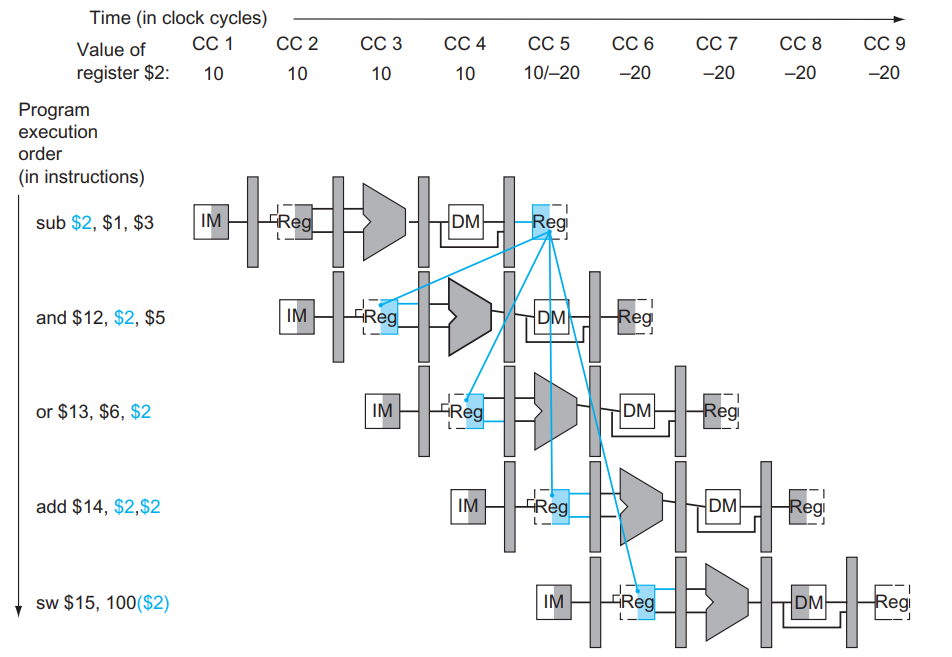
\includegraphics[width=15cm]{obrazky-figures/conflicts.png}
  \caption{Sekvence instrukcí vykonávaných ve skalární lince. \cite{OrganizationAndDesign}}
  \label{dataconflictsfrombook}
\end{figure}

\section{Vyrovnávací paměť}
\label{cache}
% todo

Paměť, která je dostatečně rychlá pro současné procesory, je zároveň velmi drahá.
Řešením tohoto problému je \emph{hierarchie pamětí} -- víceúrovňová struktura, kde úrovně blíž procesoru mají menší kapacitu, ale větší rychlost.
Výsledkem je vyvážený stav mezi výkonem a cenou. \cite{avs}

Hierarchie pamětí funguje dobře, protože přístupy do paměti nebývají zcela náhodné, ale řídí se \emph{principem lokality}.
Prvním typem lokality je časová lokalita.
Ta tvrdí, že k~paměťovým místům, ke kterým bylo přistoupeno nedávno, bude pravděpodobně v~blízké době přistoupeno znovu.

Druhým typem lokality je prostorová lokalita.
Ta předvídá, že k~fyzicky blízkým paměťovým místům se přistupuje blízko v~čase.

Pokud programy tyto principy při práci s~pamětí dodržují, mají tendenci vykazovat lepší výkon.
\cite{QuantApproach}

Hierarchie pamětí na nejrychlejší úrovni využívá registry.
Na další úrovni je vyrovnávací paměť (cache), poslední úroveň tvoří hlavní paměť.
Modely s~více úrovněmi cache jsou běžné, k~popsání základních principů se ale budu věnovat modelu s~jednou úrovní cache.
Programátor s~pamětí pracuje jako s~celkem, hierarchie pamětí se projevuje pouze rychlostí výpočtu.

Cache obsahuje části hlavní paměti (bloky) se kterými procesor momentálně pracuje.
Nové bloky jsou alokovány při čtení nebo zápisu na paměťové místo, které se v~cache momentálně nenachází.
Záznam v~cache obsahuje informaci o~původní lokaci bloku v~paměťovém prostoru, aby později mohl být vrácen do hlavní paměti.
Bloky jsou v~paměti zarovnané na násobek své velikosti.

Nejčastěji používaná strategie ukládání bloků je \emph{asociativní cache}.
Úložiště pro bloky je v~této variantě rozděleno do skupin o~$m$ blocích.
Každý blok hlavní paměti je částí své adresy (indexem) mapován na právě jednu skupinu.

Zajímavé jsou krajní případy.
Pokud $m = 1$, potom se cache nazývá přímo mapovaná.
Pokud $m$ odpovídá kapacitě cache, potom se cache nazývá plně asociativní.

Pokud ve skupině není pro nový blok místo, je nutné jeden blok vybrat, přemístit ho zpět do hlavní paměti a tím místo uvolnit.
Nejznámější strategie výběru bloku ve skupině (victim) jsou:
\begin{itemize}
    \item náhodný výběr,
    \item FIFO (výběr nejstaršího bloku),
    \item LRU (nejdéle nepoužitý blok).
\end{itemize}
Efektivita cache se vyjadřuje četností nalezení požadovaného bloku (hit rate) v~procentech.

Hledání bloku ve skupině je prováděno paralelním porovnáním jiné části adresy (tagu).
Použití částí adresy je naznačeno na obrázku \ref{cachelineaddress}.
Prvních \texttt{t} bitů je použito jako \emph{tag} k~vyhledání v~rámci skupiny.
Následujících \texttt{k} bitů adresuje skupinu a posledních \texttt{b} bitů adresuje obsah bloku.

\begin{figure}[ht]\centering
  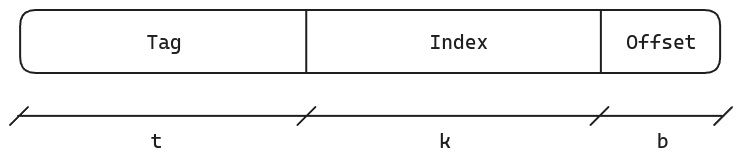
\includegraphics[width=11cm]{obrazky-figures/cacheline.png}
  \caption{Adresa paměti a její části.}
  \label{cachelineaddress}
\end{figure}

% todo víceúrovňová cache

\chapter{Superskalární procesor}
\label{superscalarchapter}
% multiple issue
% https://en.wikipedia.org/wiki/Superscalar_processor

% e performance of a computer is determined by three key
% factors: instruction count, clock cycle time, and clock cycles per instruction (CPI).
Délka výpočtu je určena třemi hlavními faktory: počtem instrukcí, frekvencí hodinového signálu a počtem instrukcí provedených za hodinový signál (\emph{Instructions Per Clock -- IPC}).
Architektura superskalárních procesorů zvyšuje výkon zvýšením IPC, typicky až nad hodnotu 1 -- jinými slovy, mohou vykonat 2 a více instrukcí ve stejný čas. \cite{QuantApproach}

Superskalární procesory rozšiřují řetězení na úrovni instrukcí ze skalárních řetězených procesorů.
K~časovému paralelismu přidávají \emph{prostorový paralelismus}, který spočívá v~rozšíření linky na $m$ instrukcí v~každém stupni a duplikací potřebných hardwarových jednotek.
Výsledkem je, že superskalární procesory mohou vydat k~výpočtu více instrukcí v~jednom taktu.
Cenou za zrychlení je zvýšení složitosti obvodu a tím nižší dosažitelný kmitočet, vyšší spotřeba energie a větší plocha čipu.

Existuje velké množství technik sloužících ke snižování doby zastavení linky.
V~této kapitole je blíže rozvedeno dynamické plánování, provádění kódu spekulativně a mimo pořadí.
Tyto koncepty bývají vysvětlovány a implementovány zároveň, pokusím se je ale vysvětlit izolovaně.
Zmíněné metody jsou pouze výběrem z~možných způsobů implementace superskalárních procesorů.

% in order superscalar
% scoreboarding??

\section{Konflikty}
\label{conflicts}

Kapitola o~skalárních procesorech (viz sekce \ref{konfliktySubSub}) definovala konflikt jako datovou závislost mezi dvěma instrukcemi.
Pro superskalární procesory je užitečné tento problém rozvést blíže.

V~případě, kdy dochází k~přeuspořádání pořadí vykonání instrukcí, je nutné uvažovat i \emph{nepravé} datové konflikty.
Pořadí pravých datových konfliktů (RAW) musí být respektováno, protože na rozdíl od nepravých nesou význam výpočtu. Jinými slovy nelze prohodit pořadí vykonání instrukcí s~pravým datovým konfliktem.

Nepravé konflikty můžeme charakterizovat jako konflikty jmen.
Vznikají znovupoužitím jména paměťového místa v~důsledku konečného počtu registrů, nebo vícenásobným vykonáním stejné instrukce.
Důležité je, že nepravou závislost lze na rozdíl od pravé závislosti odstranit bez ovlivnění správnosti výpočtu, protože mezi instrukcemi nejsou vyměňována žádná data \cite{QuantApproach}.
Nepravé závislosti lze řešit přejmenováním při tvorbě programu (programátorem nebo překladačem), nebo za běhu řídícím hardwarem procesoru.
Algoritmy Scoreboarding a Tomasulo, které jsou při řešení konfliktů využívány, uvedu v~sekci \ref{chap:ooo}.

Obrázek \ref{dataconflicts} vizualizuje pravé i nepravé konflikty mezi registry.
Nepravé konflikty jsou zobrazeny přerušovanou čarou, pravé konflikty plnou čarou.

\begin{figure}[ht]\centering
    % add a2, a0, a1
    % mul a3, a2, a1
    % sub a1, a0, a4
    % xor a3, a5, a6
  \centering
  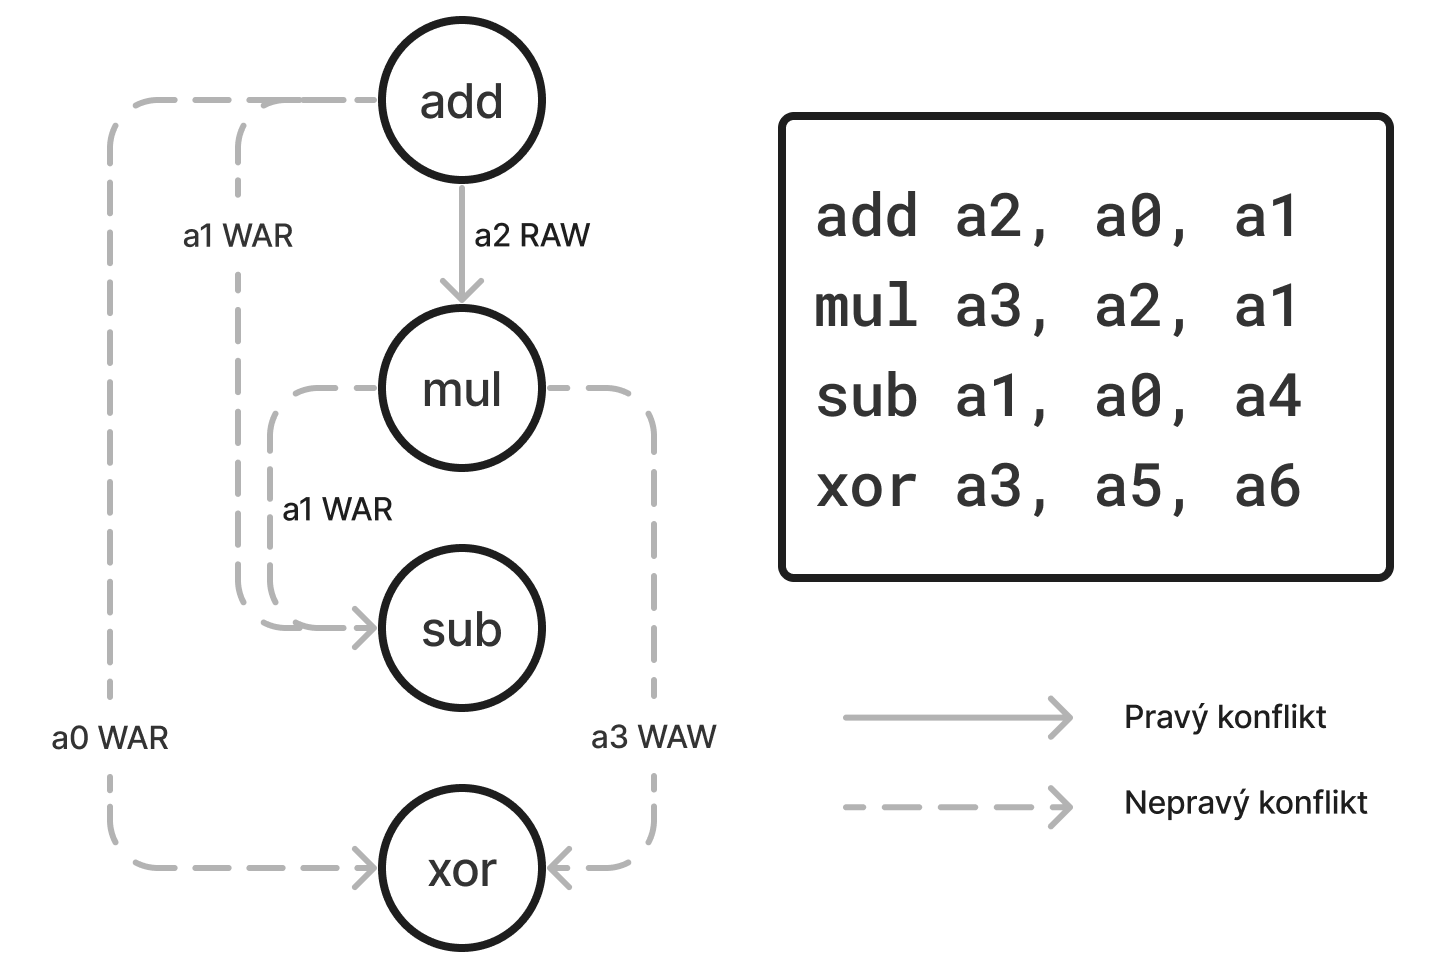
\includegraphics[width=13cm]{obrazky-figures/dataconflicts.png}
  \caption{Program a jeho datové závislosti zobrazené jako graf.}
  \label{dataconflicts}
\end{figure}

\subsection{Řídící konflikty}

Skokové instrukce manipulují programový čítač (PC).
Důsledkem je, že pořadí vykonání instrukcí je známo až při samotném výpočtu.
Adresa následující instrukce není při zřetězeném zpracování známa po prvním stupni linky (procesor nezná ani typ zpracovávané instrukce, dokud není dekódována), procesor tedy typicky předpokládá, že instrukce skoková není a začíná zpracovávat následující instrukci.

Dokud není vypočítána adresa následující instrukce, může být počítána špatná větev programu, proto je žádoucí tento výpočet urychlit.
Techniky pro eliminaci pokut skokových instrukcí zahrnují predikci skoků a předsazení výpočtu podmínky v~lince.
Pokud dojde ke zpracovávání nesprávné instrukce, musí být z~linky odstraněna.

\subsection{Strukturní konflikty}

Ke strukturnímu konfliktu dochází, pokud vykonání dvou instrukcí vyžaduje stejný prostředek.
Prostředkem je myšlen hardwarový modul, například funkční jednotka, nebo zápisová brána.

Tento typ konfliktu se řeší serializací zpracování, neboli čekáním.
Dopady konfliktů se zmenšují znásobením hardwaru, například přidáním více aritmetických jednotek (ALU).

\section{Zpracování instrukcí mimo pořadí}
\label{chap:ooo}
% https://stackoverflow.com/questions/10074831/what-is-general-difference-between-superscalar-and-out-of-order-ooo-execution
% https://stackoverflow.com/questions/49601910/out-of-order-execution-vs-speculative-execution

Většina procesorů se zpracováním mimo pořadí jsou zároveň superskalární, ale nemusí být nutně.
Během výpočtu musí být zachována platnost programovacího modelu, který říká, že projevy instrukcí musí být aplikovány v~pořadí.
Zpracování instrukcí mimo pořadí dovoluje provádět práci na jiných instrukcích, než ta, která je právě v~pomyslné lince na řadě, aniž by model porušila.

Instrukce nemohou být vykonávány v~libovolném pořadí, algoritmus musí instrukci označit jako připravenou k~vykonání.
Analýza závislostí spočívá v~detekci datových konfliktů registrů tak, jak je popsána v~předešlé sekci \ref{conflicts}.
Komplikace nastává u~paměťových operací -- konflikty RAW, WAW a WAR nelze odhalit analýzou závislostí registrů, protože konflikty vznikají v~hlavní paměti a mohou být ověřeny až jsou vypočítány adresy. 

% limited OOO - předbíhání jen některého druhu (load before load)
Aby byla dodržena sémantika programu a zároveň bylo umožněno vykonávat paměťové instrukce mimo pořadí, je v~procesorech zaveden koncept \emph{relaxované paměťové konzistence} \cite{avs}.
Čtení a zápisy se mohou přeuspořádat, pokud není narušena správnost programu.
Pokud je z~nějakého důvodu nutné vynutit pořadí paměťových operací, je nutné vložit explicitní bariéry.
Paměťové instrukce za bariérou se začnou vykonávat až jakmile jsou všechny paměťové instrukce před bariérou dokončeny.
% release, acquire, ...

Linka procesoru se dělí na dvě části. 
Front-end superskalárního procesoru odpovídá stupňům Instruction Fetch (IF) a Instruction Decode (ID).
Back-end odpovídá stupňům Execute (EX), Memory Access (MA) a Write Back (WB).
Front-end pracuje v~pořadí programu.
Back-end pracuje mimo pořadí programu (OOO -- out of order), instrukce back-end opouští opět v~původním pořadí.
V~rámci back-endu se mohou libovolně promísit přístupy do paměti a vykonávání všech instrukcí v~okně. Stále ale musí být respektovány datové závislosti.

% fáze vydání nebo potvrzení?
V~cyklu zpracování instrukce přibývá fáze potvrzení instrukce (\emph{instruction commit}).
Vydání proběhne jakmile je instrukce na řadě a výsledek je vypočítán.
Výsledkem vydání je propsání do vnějšího stavu procesoru.

Procesor identifikuje nezávislé instrukce a vykoná je paralelně.
Tím snižuje počet zastavení linky a zvyšuje IPC.

Skokové instrukce představují asi 20\% instrukcí programu.
Z~toho vyplývá, že okno instrukcí, o~kterých víme, že budou vykonány, je příliš malé.
Proto bývá zpracování mimo pořadí nejčastěji spojeno se spekulativním vykonáváním. 

% todo komplikace se závislostmi v hlavní paměti
% mělo by to být zde, v konfliktech, nebo v spekulaci?

\subsection{Reorder Buffer}

Pokud jsou instrukce vykonávány mimo pořadí, musí být v~hardwaru udržena informace o~původním pořadí.
Za tímto účelem back-end obsahuje \emph{Reorder Buffer} (ROB).
Jedná se o~cyklický buffer s~typickou kapacitou 100-200 položek \cite{avs}.
Instrukce, jejich výsledky a související příznaky jsou zde uchovávány v~programovém pořadí.

Do fáze commit vstupují instrukce na čele ROB.
Jakmile instrukce opustí ROB, přestává být spekulativní.
Výsledek instrukce je propsán do architekturních registrů a instrukce je považována za potvrzenou.

Zaplněním ROB vzniká strukturní konflikt a předchozí fáze linky se musí pozastavit.

\subsection{Algoritmus Tomasulo}
% dynamic scheduling
% Reservation Stations
% Register Renaming
% Handling Dependencies

Dva nejznámější algoritmy pro dynamické plánování instrukcí jsou \emph{ScoreBoarding} a \emph{Tomasulo}.
ScoreBoarding má velká omezení\footnote{ScoreBoarding je omezen na plánování v~rámci \emph{basic bloku} instrukcí, WAW a WAR konflikty řeší čekáním.}, proto blíže rozvedu pouze algoritmus Tomasulo.

Hlavním hardwarovým prvkem algoritmu je \emph{rezervační stanice} (RS), buffer pro ukládání operandů.
RS může být centrální, nebo individuální pro každý druh instrukcí.
Položka RS má následující pole:
\begin{itemize}
    \item \emph{busy bit}  -- příznak, zda je položka obsazena a validní,
    \item \emph{operace}   -- druh operace (například sčítání),
    \item \emph{operandy}  -- trojice (hodnota, tag, valid),
    \begin{itemize}
        \item \emph{hodnota} -- kopie hodnoty operandu,
        \item \emph{tag}     -- ukazatel na registr operandu,
        \item \emph{valid}   -- příznak, zda je pole hodnota validní,
    \end{itemize}
    \item \emph{destinace} -- ukazatel na registr, do kterého má být výsledek zapsán.
\end{itemize}
Tato struktura řeší konflikty RAW -- instrukce je poslána do funkční jednotky až v~moment, kdy jsou všechny operandy připraveny.

Konflikty WAR a WAW jsou vyřešeny \emph{přejmenováním registrů}.
Podstata těchto falešných konfliktů není datová, jedná se o~\emph{konflikt jmen}.
Výsledek každé instrukce se zapíše do nového, unikátně pojmenovaného registru.
Dekódované instrukce místo původních jmen operandů použijí jejich nejaktuálnější přejmenování.
S~novými jmény registrů v~kódu zůstanou pouze pravé RAW konflikty.

K ilustraci přejmenování poslouží obrázek \ref{fig:renaming}.
Všimněte si, že vstupní registry používají nejaktuálnější přejmenování a výstupní registry vytvoří nové přejmenování.

\begin{figure}[ht]
     \centering
     \begin{subfigure}[b]{0.4\textwidth}
         \centering
         \begin{lstlisting}
        add     x2, x1, x1 
        sub     x2, x2, x3 
        mul     x4, x5, x2 
        shr     x5, x1, x4 
\end{lstlisting}
         \caption{Původní jména operandů.}
         \label{fig:renaming1}
     \end{subfigure}
     \hfill
     \begin{subfigure}[b]{0.4\textwidth}
         \centering
         \begin{lstlisting}
        add     t0, x1, x1 
        sub     t1, t0, x3 
        mul     t2, x5, t1 
        shr     t3, x1, t2 
\end{lstlisting}
         \caption{Jména operandů po přejmenování.}
         \label{fig:renaming2}
     \end{subfigure}
        \caption{Přejmenování registrů.}
        \label{fig:renaming}
\end{figure}

Je nutné v~hardware udržovat informaci o~posledním přejmenování architekturních registrů, a to ze dvou důvodů: (1) přejmenování operandů nových instrukcí a (2) propsání výsledků při propouštění instrukcí.
Implementace přejmenování vyžaduje dva prvky.
Prvním je tabulka RAT (\emph{Register Alias Table}).
RAT implementuje mapování jmen architekturních registrů na jejich nejaktuálnější přejmenování.

Druhým prvkem je úložiště spočtených výsledků.
Zde jsou možné dvě implementace.
Ve variantě přejmenování v~ROB položky ROB obsahují spočtenou hodnotu instrukce.
Výsledek je ve fázi commit propsán do architekturního registru.

Druhou variantou je přejmenování v~RRF (\emph{Rename Register File}).
Zde se výsledky ukládají do velkého pole registrů.
Pole může být spojeno s~polem architekturních registrů, v~takovém případě propsání do architekturního registru proběhne přepsáním ukazatelů do pole.

Komunikace výsledků probíhá přes sdílenou sběrnici.
Funkční jednotky na sběrnici posílají výsledky; pole registrů, ROB a RS naslouchají a aktualizují své hodnoty.

\subsection{Load/Store jednotka}
\label{ooo_ls}
% pouze aspekty pro ooo, ne spekulaci
% https://compas.cs.stonybrook.edu/~nhonarmand/courses/sp15/cse502/slides/11-ooo_mem.pdf

Podpora vykonávání paměťových instrukcí mimo pořadí vyžaduje speciální hardware.
Instrukce load a store musí být udržovány v~programovém pořadí, v~tabulkách Load Buffer a Store Buffer.

Položka v~Load Bufferu obsahuje vypočtenou adresu.
Adresa může být vypočtena mimo pořadí.
Load může načíst z~paměti, pokud jsou všechny adresy předchozích instrukcí store vypočteny a nepřekrývají se s~loadem.
Pokud je nalezen store se stejnou adresou a položka store bufferu obsahuje zapisovanou hodnotu, může proběhnout optimalizace předání hodnoty, čímž se ušetří jedno čtení z~paměti.
% jak se zjišťuje alias u čtení 1B vs 8B?

Instrukce store může být vykonána, pokud je na čele ROB.

\section{Spekulativní zpracování instrukcí}
% reducing pipeline stalls
% maximize the utilization of execution units

% todo RRF, jak do toho zapadá

% může být skalární spekulace? může
Koncept spekulativního vykonávání jsem již zmínil v~sekci \ref{branchpredict} o~předpovědi skoků.
Při spekulativním vykonávání se spekuluje o~řízení programu, datech a paměťových závislostech.
Instrukce, jejíž výsledek byl předpovězen, je zpracována spolu s~ostatními instrukcemi a běžným výpočtem se zkontroluje, zda byla predikce správná. \cite{QuantApproach}

Kontrola probíhá ve fázi potvrzení instrukce.
Touto fází projdou pouze instrukce, které jsou jistě produktem správné předpovědi.
Pokud predikce odpovídá výsledku, je možné pokračovat ve výpočtu.
Pokud predikce selhala, je nutné všechny následující instrukce označit za nesprávné a smazat jejich rozpočítané výsledky.
Smazat výsledky je nutné, protože mohou být produktem jiných nesprávných výsledků.
% todo je nějaký dependency analysis moc drahý?

% todo poznámka o výjimkách
Výjimky se také musí projevit až v~momentě potvrzení instrukce, protože do té doby není jisté, zda se instrukce skutečně má vykonat. 
Aby bylo možné spekulovat, výsledky výpočtu tedy musí být možné \emph{navrátit}.

Hlavním předpokladem spekulativního vykonávání je ten, že předpovědi mají vysokou úspěšnost.
Každá špatná predikce znamená, že se výpočetní výkon vynakládá na výpočet špatných instrukcí, nebo špatných hodnot operandů.

\subsection{Předvídání skoků}

Při spekulaci o~větvení do linky vstupují a jsou zpracovávány instrukce, o~kterých nemusí být jisté, jestli jsou pro výpočet nutné a že zpracovány být mají.

Superskalární procesor načítá více instrukcí v~jednom taktu.
To znamená, že v~jednom taktu může načíst více než jednu skokovou instrukci.
Fetch jednotka musí být schopna buď zastavit načítání před druhou skokovou instrukcí, nebo musí vypočítat více predikcí v~rámci jednoho taktu.

Detailněji bude předvídání skoků rozvedeno v~sekci \ref{branchpredict}.

\subsection{Předvídání čtení z~paměti}
% https://en.wikipedia.org/wiki/Memory_disambiguation
% https://en.wikipedia.org/wiki/Memory_dependence_prediction

Spekulativní provádění paměťových operací sebou nese komplikaci: efekt spekulativního zápisu do paměti (nebo cache) se nesmí projevit, dokud instrukce není potvrzena (z~důvodu špatné predikce, nebo výjimky).
Z~toho důvodu se data zapisují do Store Bufferu a do paměti se zapisují až při potvrzení instrukce.  
% zmíňka o tom, že spekulativní load taky mění stav (cache), viz spectre

Verzi popsanou v~sekci \ref{ooo_ls} lze rozšířit spekulací.
Instrukce load již nemusí čekat na všechny adresy starších instrukcí store, ale mohou spekulovat, že u~žádné z~instrukcí store s~nedopočítanou adresou k~překrytí nedojde.
Nejjednodušší strategií je spekulovat, že k~překrytí nedojde nikdy.
Ta funguje dostatečně dobře, protože pravděpodobnost pravé závislosti je malá.
Složitější prediktory nebývají v~praxi používány. 
\cite{moshovos1998memory}
% https://ftp.cs.wisc.edu/sohi/theses/moshovos.pdf

Tato spekulace je ověřena, když je store propouštěn.
Adresa store je porovnána s~položkami v~Load Bufferu, v~případě shody jde o~špatnou spekulaci a stejně jako u~spekulace se skoky se vypláchne ROB.

% TODO když bude chuť, ale nepoužívá se v simulátoru
% \subsection{Předvídání hodnot}
% https://hal.science/hal-03325303/document

\section{Předvídání skoků}
\label{branchpredict}

Předpověď skoku má dva komponenty: předpověď podmínky skoku a předpověď cílové adresy skoku.
Předpověď podmínky se nevztahuje pouze na podmíněné skokové instrukce.
U~nepodmíněných skoků je sice jisté, že se skok má provést, jednotka fetch ale sama o~sobě nemůže identifikovat instrukci jako nepodmíněný skok -- instrukce je dekódována až ve fázi decode.
Z~tohoto důvodu prediktory pracují s~\emph{adresou instrukce}.

% první encounter
Při prvním zpracování instrukce na nové adrese není známo, zda se jedná o~instrukci skokovou.
Proto je jedinou možností pokračovat ve zpracování sekvence instrukcí.

Při následujících načteních skokových instrukcí již o~nich existuje záznam a je možné skok předpovídat.

% zotavení
Předpověď musí být ověřena porovnáním s~výsledkem klasického výpočtu skoku.
Při případném zjištění nesprávné předpovědi skoku musí být všechny následující rozpočítané instrukce z~linky vypláchnuty.
Po vypláchnutí linky je registr PC opraven na správný cíl skoku a procesor může pokračovat ve výpočtu.
Nesprávně může být předpovězen i cíl skoku.
V~klasické skalární lince jsou instrukce ze špatně předpovězené větve zrušeny dříve, než jsou vykonány.
% taky feedback pro dynamický prediktor
% todo - je zde nějaká pokuta kromě zahození výsledků?

% možná zmínka o vykrytí branch delaye užitečnou prací při překladu - a delayed branch (MIPS)

\subsection{Předpověď podmínky skoku}

V~této sekci budu používat pojmy \emph{pozitivní a negativní predikce} pro označení situace, kdy prediktor vyhodnotí, že je nebo není splněna podmínka dané skokové instrukce.

Strategie pro predikci podmínky skoku se dělí na dvě skupiny -- statické a dynamické.
Jejich rozdíl v~tom, že dynamické strategie k~predikci používají informace o~chování za běhu programu, typicky historií větvení.
\cite{branchStrategies}

\subsubsection{Statické předpovědi}

Nejjednodušší verzí předpovědi podmínky skoku je statická negativní predikce.
V~tomto případě je vždy načtena následující instrukce a není potřeba předpovídat cíl skoku.
Statická pozitivní predikce může mít vyšší úspěšnost.

% static, cold branches
Jiné statické strategie mohou brát ohled na operační kód instrukce.
Prediktor může například instrukce \texttt{beq} předpovídat negativně a instrukce \texttt{blt} předpovídat pozitivně.
Operační kód instrukce může obsahovat příznak, kterým se prediktor může řídit.
Předpověď v~tomto případě učinil překladač, profilovací nástroj, nebo programátor. \cite{branchStrategies}

Další strategie mohou využít směru skoku (skok dopředu nebo dozadu), nebo vzdálenosti skoku.
Směr skoku je zajímavým ukazatelem, protože v~mnoha programech velkou část skoků směrem zpět tvoří smyčky, které typicky provádějí velký počet iterací.
Nevýhodou je, že předpověď cílové adresy a podmínky nemůže být provedena paralelně.

Statické strategie mají příliš malou úspěšnost pro použití v~současných procesorech.

\subsubsection{Dynamické předpovědi}

Dynamická predikce skoků mění verdikt v~průběhu programu.
Stav prediktoru udržuje historií větvení, znalost historie se používá k~predikci větvení.
V~ideálním případě by každá instrukce (adresa) měla vlastní stav prediktoru, z~praktických důvodů se ale tabulka těchto stavů s~názvem Branch History Table (BHT) adresuje částí adresy v~registru PC.
Pokud je tabulka vůči kódu malá, může dojít ke sdílení stavu prediktoru více instrukcemi. \cite{OrganizationAndDesign}
% todo lze taky použít lru, fifo?
% také lze hashovat

Dynamické prediktory se umí naučit různé vzory \cite{avs}.
Nejjednodušší možností dynamické predikce je predikce na základě stavového automatu.
Podle počtu stavů se prediktory označují jako 1 bitový (2 stavy) nebo 2 bitový (4 stavy), oba jsou znázorněny na obrázku \ref{fsmpredictor}.
Stavy zde představují saturační čítač.

Z~aktuálního stavu je potom odvozena předpověď.
Pokud je aktuální stav v~pravé polovině automatu, potom se skočit má, jinak se předpovídá neskočit.
Přechod do nového stavu se uskuteční při zpětné vazbě prediktoru. Přechod označený \uv{1} znamená, že skok se doopravdy uskutečnil, přechod \uv{0} znamená, že ke skoku nemělo dojít.

\begin{figure}[ht]\centering
% digraph finite_state_machine {
% 	fontname="Helvetica,Arial,sans-serif"
% 	node [fontname="Helvetica,Arial,sans-serif"]
% 	edge [fontname="Helvetica,Arial,sans-serif"]
% 	rankdir=LR;
% 	node [shape = circle];
% 	0 -> 0 [label = "0"];
% 	0 -> 1 [label = "1"];
% 	1 -> 0 [label = "0"];
% 	1 -> 1 [label = "1"];
	
% 	00 -> 01 [label = "1"];
% 	01 -> 10 [label = "1"];
% 	10 -> 11 [label = "1"];
	
% 	01 -> 00 [label = "0"];
% 	10 -> 01 [label = "0"];
% 	11 -> 10 [label = "0"];
	
% 	00 -> 00 [label = "0"];
% 	11 -> 11 [label = "1"];
% }
  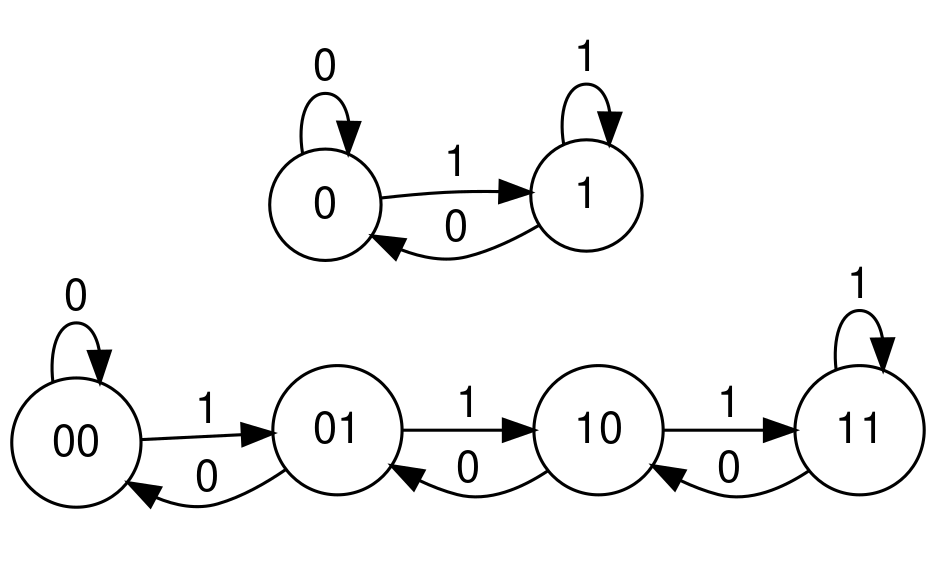
\includegraphics[width=10cm]{obrazky-figures/fsmpredictors.png}
  \caption{Schéma 1-bitového prediktoru (nahoře) a 2-bitového prediktoru (dole). }
  \label{fsmpredictor}
  % http://magjac.com/graphviz-visual-editor/
\end{figure}

% feedback, learning period
Dynamickým prediktorům je poskytována zpětná vazba v~podobě informace o~úspěšnosti poslední predikce.
V~případě stavového automatu se stav posune po hraně značené \uv{+}, pokud byla predikce ověřena jako správná, nebo \uv{-} v~opačném případě.
Stavy prediktorů jsou inicializovány na určitou počáteční hodnotu.
První predikce mohou mít špatnou úspěšnost.
Tato fáze se nazývá učící období (learning period).
Po naučení vzoru se úspěšnost prediktoru ustálí.
Každý druh prediktoru je schopen naučit se pouze určitou podmnožinu vzorů.

% Adaptivní prediktor
% todo je ta historie globální, nebo pro instrukci?
Další variantou dynamických prediktorů je \emph{adaptivní prediktor}.
K~predikci větvení jsou použity dvě informace: (1) historie posledních $k$ výsledků větvení dané instrukce a (2) záznam o~chování skokové instrukce v~minulých případech, kdy této instrukci předcházela stejná historie skoků.
Implementace spočívá v~$k$ bitovém posuvném registru historie skoků a tabulce Pattern History Table (PHT): $2^k$ prediktorů pro každou instrukci.
Konkrétní prediktor je adresován vektorem historie a adresou instrukce. \cite{adaptiveBranch}

% todo Korelační prediktor
% adaptivní ale s globální historií
Korelační prediktor místo lokální historie používá jedinou, globální historií.

\subsection{Předpověď cílové adresy skoku}

% BTB, BTAC
K~predikci cílové adresy skoků se využívá cache nazývaná Branch Target Buffer (BTB).
Tato tabulka se indexuje adresou skokové instrukce.

% komplikace s call - RSB
Komplikací jsou nepřímé skokové instrukce, neboli instrukce, jejichž cíl skoku není konstantní.
Takové skoky jsou využívány hlavně při návratu z~funkce (\texttt{ret}), nebo při práci s~ukazateli na funkce.
Predikce by byla nepřesná, protože funkce bývá volána z~několika míst.
Úspěšnost lze zlepšit zásobníkem Return Stack Buffer (RSB), na který se při vstupu do funkce adresy ukládají a při opouštění vybírají.

% loop counter?

\chapter{Architektura RISC-V}
\label{riscvchapter}
% todo ABI

RISC-V je otevřená instrukční sada architektury RISC.
Původně byla vyvinuta na UC Berkeley pro výukové účely.
Instrukční sada je navržena pro maximální jednoduchost a rozšiřitelnost, s~cílem mít malé požadavky na hardware implementace.
\cite{riscvspec}

Definuje registry, samotnou instrukční sadu, její kódování a rozšíření, konvenci volání (ABI), výjimky.
Paměťový systém je navržen jako liitle-endian.
Specifikace připouští varianty s~big-endian nebo oba systémy současně.

% general-purpose register computer
% Type Register-register (0, 3) - 0 memory operands, max 3 alu operands (one output)
% register, immediate, displacement addressing

\section{Architektura RISC}
% RISC a CISC

Architektury RISC (\emph{Reduced Instruction Set Computer}) kladou důraz na jednoduchost hardwaru, který instrukční sadu implementuje a na malou spotřebu energie.
Díky důrazu na nízkou cenu, malé ploše čipu a malému příkonu se často objevuje v~malých zařízeních poháněných bateriemi, například v~IoT a mobilních telefonech.

RISC se vyznačuje menším počtem instrukcí.
Typicky se jedná o~minimální množinu instrukcí, ve které je možné popsat výpočty a práci s~hardwarem.
Do instrukční sady se ale dostávají i další instrukce.
Zajímavostí a extrémním případem je instrukce \href{https://developer.arm.com/documentation/dui0801/h/A64-Floating-point-Instructions/FJCVTZS}{FJCVTZS} instrukční sady ARM.
Jde o~instrukci pro specifický převod čísla float64 na celé číslo.
Tento výpočet je možné provést kombinací jiných instrukcí.
Důvodem přidání této složitější instrukce do instrukční sady navzdory filozofii RISC byl výkon v~důležitém případu užití -- tuto konverzi často provádějí interprety JavaScriptu.

% https://stackoverflow.com/questions/50966676/why-do-arm-chips-have-an-instruction-with-javascript-in-the-name-fjcvtzs
% https://community.arm.com/arm-community-blogs/b/architectures-and-processors-blog/posts/armv8-a-architecture-2016-additions#:~:text=number%20signed%20addition-,Improved%20Javascript%20data%20type%20conversion,-Javascript%20uses%20the

Situace s~menším množstvím instrukcí se dá vylepšit makry v~assembleru, takzvanými \emph{pseudoinstrukcemi}.
Pseudoinstrukce jsou lexikální náhradou za instrukce s~bližším sémantickým významem.
Tabulka \ref{table:pseudoins} uvádí několik příkladů.
Instrukční sadu je možné tímto způsobem virtuálně rozšířit.
V~současném stavu, kdy je naprostá většina strojového kódu generována překladači, ale programátorský komfort není menší instrukční sadou negativně ovlivněn.

\begin{table}[ht]
\centering
\begin{tabular}{|l|l|l|}
\hline
Pseudoinstrukce    & Ekvivalent z~instrukční sady & Význam                         \\ \hline\hline
mv rd, rs          & addi rd, rs, 0     & Kopírování hodnoty             \\ \hline
neg rd, rs         & sub rd, x0, rs     & Negace celého čísla            \\ \hline
bgt rs, rt, offset & blt rt, rs, offset & Skok, pokud rs\textgreater{}rt \\ \hline
\end{tabular}
\caption{Příklady pseudoinstrukcí a jejich odpovídajících reálných instrukcí.}
\label{table:pseudoins}
\end{table}

Kódování instrukcí je optimalizováno pro jednoduché načítání a dekódování.
Kódování mívá fixní délkou (např. 4\,B), operační kód a operandy jsou zapsány na předvídatelných místech v~kódu.
Jednodušší dekódování znamená, že k~jeho implementaci je zapotřebí méně hardwarových obvodů a čip má menší spotřebu.

Protipólem je architektura CISC (\emph{Complex Instruction Set Computer}), která definuje větší množství instrukcí.
Jedna instrukce může představovat i složitější operace, například aritmetickou operaci a načtení z~paměti. Kódy mají typicky proměnlivou délku kódování.
Častěji používané operace mají kratší kódy, což se může projevit kompaktnější reprezentací programu v~paměti.

Některé implementace CISC v~rámci fáze dekódování převádí instrukce na sekvenci \emph{mikro-instrukcí}, další části linky dále operují s~touto reprezentací.
Mikro-instrukce více připomínají instrukční sadu RISC.
Dekódování je složitější a proto má větší nároky na hardware.

\section{Instrukční sada}

Specifikace definuje základní celočíselnou sadu instrukcí ve dvou šířkách registrů, 32 bitů (\texttt{RV32I}) a 64 bitů (\texttt{RV64I}).
Verze \texttt{RV64I} je analogická s~\texttt{RV32I}, s~tím rozdílem, že registry mají šířku 64 bitů.
Procesor musí implementovat alespoň jednu z~těchto dvou sad a libovolné množství rozšíření.
Dále budu popisovat pouze 32-bitovou variantu.

Z~pohledu programátora je stav procesoru vyjádřen 31 obecnými registry pojmenovanými \texttt{x1}-\texttt{x31} a speciálními registry \texttt{x0} a \texttt{pc}.
Registr \texttt{x0} obsahuje konstantní hodnotu 0, registr \texttt{pc} obsahuje ukazatel na aktuální instrukci.

Základní instrukční sada definuje aritmetické instrukce, řídící instrukce a instrukce pro práci s~pamětí.
Aritmetické instrukce nevyvolávají výjimky a nekontrolují přetečení.
Přetečení je možné zkontrolovat explicitní podmínkou.
Kódování instrukcí dovoluje vyjádřit přímé hodnoty v~rozsahu 12 bitů.
Načtení 32 bitové konstanty je nutné provést kombinací instrukcí \texttt{LUI} a \texttt{ADDI}.

Skokové instrukce umožňují podmíněné a nepodmíněné relativní skoky.
Skok na absolutní adresu je možný kombinací instrukcí \texttt{LUI} a \texttt{JALR}.
Instrukce musí být zarovnané, proto skok na nezarovnanou adresu vyvolá výjimku.
Uložení návratové adresy provádí instrukce \texttt{JAL}.
Instrukce pro podmíněné skoky provádějí komparaci dvou registrů, vykonávají tedy dvě operace -- \emph{compare} a \emph{branch}.
% https://github.com/emb-riscv/specs-markdown/blob/develop/exceptions-and-interrupts.md#exceptions

Reprezentace instrukce v~paměti zabírá 4 bajty, je zarovnaná na 4 bajty a je zakódována v~jednom ze čtyř formátů\footnote{Rozšíření C navíc definuje komprimované 16-bitové instrukce}.
Formáty mají společné pole pro \emph{opcode} a 5-bitové adresy operandů-registrů.
Liší se ve využití zbylého prostoru, který je interpretován buď jako přímá hodnota, nebo další část \emph{opcode}. \cite{riscvspec}

% privileged specs
Specifikace RISC-V je rozdělena na dvě části.
Druhá část definuje privilegovaný režim, který je nutný k~provozu operačního systému.
Architektura poskytuje tři režimy: Machine (M), Supervisor (S) a User (U).

Speciální registry (\emph{control and status registers} -- CSR) slouží ke sběru statistik a ladění.
Jejich čtení a nastavování je umožněno speciálními systémovými instrukcemi.
Jejich zápis je také vyvolán jako vedlejší efekt vykonávání instrukcí.
Instrukce \texttt{ECALL} slouží k~žádosti o~obsloužení jádrem.
Obdobně jako instrukce \texttt{SYSCALL} z~ISA x86, argumenty jsou definovány podle používaného ABI.

\subsection{Rozšíření instrukční sady}
% rozšíření
Důležitou vlastností RISC-V je rozšiřitelnost.
Jednodušší čipy mohou implementovat pouze ta rozšíření, která ke svému účelu nutně potřebují.
Případně mohou jednoduše specifikovat vlastní instrukce relevantní pro svou doménu.

% genreal IMAFD
Rozšíření implementovaná daným zařízením jsou specifikována základní sadou a výčtem rozšíření.
Typickou sadu rozšíření vyjadřuje zkratka \texttt{RV32IMAFD}, také nazývanou \texttt{RV32G}.
Významy těchto rozšíření jsou uvedeny v~tabulce \ref{table:extensions}.

\begin{table}[ht]
\centering
\begin{tabular}{|c|l|}
\hline
Zkratka  & Popis rozšíření             \\ \hline\hline
M          & Celočíselné násobení a dělení     \\ \hline
A~& Atomické instrukce     \\ \hline
F         & podpora čísel \emph{single} podle standardu IEEE 754-2008\footnote{ANSI/IEEE Std 754-2008, IEEE standard for floating-point arithmetic, 2008.}     \\ \hline
D         & podpora čísel \emph{double} podle standardu IEEE 754-2008     \\ \hline
\end{tabular}
\caption{Nejvýznamnější rozšíření instrukční sady RISC-V. Celý výčet je k~dispozici ve specifikaci RISC-V \cite{riscvspec}.}
\label{table:extensions}
\end{table}

% výčet rozšíření

RV32E je varianta základní instrukční sady, která má pouze 16 obecných registrů.
Je určena pro čipy s~velmi malou plochou.

\section{Paměťový model, vlákna}

RISC-V definuje 32-bitový paměťový prostor.
Přístupy do paměti nemusí být zarovnané, ale nezarovnané přístupy nemusí být atomické.

% RISC-V uses a memory model called “RVWMO” (RISC-V Weak Memory Ordering)
RISC-V používá paměťový model \emph{RISC-V Weak Memory Ordering} (RVWMO).
V~tomto modelu může jádro pozorovat paměťové instrukce jiného jádra v~jiném než původním pořadí.
Pro komunikaci vláken prostřednictvím sdílené paměti musí proto být zavedena synchronizace.
Rozšíření A~k~tomuto účelu představuje instrukce pro atomické paměťové operace.
Instrukce \texttt{FENCE} umožňuje realizovat paměťovou bariéru a tím vynutit pořadí paměťových operací.
% FENCE synchronisation, chapter 6 of manual
% todo je toto faktuální?

% todo komunikace s memory mapped i/o

\section{Aplikační binární rozhraní}
% https://github.com/riscv-non-isa/riscv-elf-psabi-doc/blob/master/riscv-abi.adoc

Aplikační binární rozhraní definuje konvenci volání a specifika RISC-V pro formáty ELF a~DWARF.
Předepisuje také velikosti a zarovnání pro datové typy jazyka C.
\cite{riscvabi}

Konvence volání označuje způsob komunikace vstupů a výstupů mezi procedurami.
Při popisu se používají aliasy pro jména registrů.
Tato jména odrážejí funkci registru v~konvenci volání.
Například registr \texttt{x2} se také nazývá \texttt{sp} (stack pointer), jelikož ukazuje na vrchol zásobníku.
Pro každý registr je specifikováno, zda má volání procedury zachovat jeho hodnotu, nebo je možné ji přepsat.

RISC-V ABI preferuje předávání argumentů registry.
Celočíselné argumenty se předávají registry \texttt{a0}-\texttt{a7}.
Pro čísla s~plovoucí desetinnou čárkou se používají registry \texttt{fa0}-\texttt{fa7}.
Pokud počet registrů nestačí, další argumenty se předávají \emph{zásobníkem}.

%
% Webová rozhraní
%

\chapter{Webová rozhraní}
\label{webchapter}
% Significance of Web Development

Webový prohlížeč a webové technologie se v~posledních letech staly uživateli očekávaným standardem pro interakci s~počítačem.
Pokud aplikace dokáže splnit své požadavky v~prostředí prohlížeče, potom je pro vývojáře výchozí volbou.
Hlavním důvodem popularity je distribuce -- uživatelé mohou aplikaci najít a začít okamžitě používat.
Vývoj webové aplikace je také rychlejší a levnější než vývoj na alternativních platformách.
% TODO nemuzu najit source

% v posledních letech se hranice začínají ztrácet. Mnoho desktopových aplikací je implementováno za pomoci webových technologií.

S~rostoucí popularitou, implementací nových standardů a vývojem rámcových řešení podíl webových aplikací stále roste.
Mnohé desktopové programy a mobilní aplikace jsou také implementovány webovými technologiemi.
% https://survey.stackoverflow.co/2023/#technology  ??

\section{Základní koncepty a technologie}
% browser, HTTP, HTML, CSS, JS, React
% Frontend vs Backend
% frameworky, bundling, polyfills

Základem obsahu na World Wide Web jsou \emph{hypermédia}.
Hypermediální dokumenty jsou spojeny navigovatelnými referencemi, takzvanými \emph{hyperlinky}.
Společně tvoří síť propojených informací, kde uživatelé mohou pohodlně přecházet mezi jednotlivými stránkami a získávat různorodý obsah, například ve formě textu nebo videa.
Dokumenty mohou být interaktivní -- tímto způsobem jsou implementovány složitější webové aplikace.

Dokumenty, jejich reprezentace a způsob jejich renderování jsou definovány kolekcí standardů vyvinutých WHATWG. Hlavním standardem je HTML Standard, který definuje jazyk HTML a některá API jako například \texttt{localStorage}.
Standard se dále odkazuje na velké množství dalších standardů, např. HTTP, CSS, Unicode, XML a standardy obrazových formátů. \cite{htmlStandard}
% Cascading Style Sheets Level 2 Revision 2, B. Bos, T. Çelik, I. Hickson, H. Lie. W3C.
% Hypertext Transfer Protocol (HTTP/1.1): Message Syntax and Routing, R. Fielding, J. Reschke. IETF.

Tyto standardy jsou implementovány webovými prohlížeči.
Prohlížeč má roli hypermediálního klienta.
Jeho prvním úkolem je komunikovat se servery v~síťové architektuře \emph{klient-server}, ve které klienti poptávají zdroje od speciálních účastníků sítě -- serverů.
Zdroji jsou v~případě webu myšleny hypertextové dokumenty, multimédia a další soubory.
Komunikace mezi uzly je rozvedena v~následující sekci.

Druhým úkolem prohlížeče je tyto dokumenty zobrazovat uživateli.
Uživatelská rozhraní blíže rozvedu v~sekci \ref{ui_scripting}.

\subsection{Přenosové protokoly}
% main concepts of HTTP

Výměna dokumentů mezi serverem a klientem probíhá bezstavovým textovým protokolem \emph{HTTP}.
Jedná se o~protokol typu request/response aplikační vrstvy.
Využívá transportní protokol TCP, poskytuje tedy spolehlivý přenos.

Zdroje jsou na webu identifikované pomocí \emph{Uniform Resource Identifier} (URI).
V~hlavičce zprávy typu request se přenáší verze protokolu, metoda, URI požadovaného zdroje, hlavičky s~informacemi o~klientovi a požadovaném zdroji a v~některých případech i tělo zprávy s~libovolnou sekvencí bajtů.
Server odpovídá zprávou response, která obsahuje statusový kód, hlavičky a data určitého typu.
\cite{http-rfc}

HTTP poskytuje několik sémantických metod.
Metody \texttt{GET} a \texttt{HEAD} slouží k~získání dokumentů.
Metodami \texttt{DELETE}, \texttt{POST} a \texttt{PUT} klient žádá server o~provedení nějakého \emph{vedlejšího efektu}, například přidání nového příspěvku na sociální síť.

Trojciferný statusový kód odpovědi indikuje, zda byl příspěvek zpracován.
Konkrétní kódy mají specifické významy, dělí se do pěti skupin: informační, úspěchové, přesměrovací, chybové na straně klienta a chybové na straně serveru.

% QUIC
Požadavky na web se neustále vyvíjí a existuje poptávka po alternativních protokolech.
Protokol HTTP se vyvíjel do verze 2 a 3.
Firma Google představila vlastní protokol QUIC, který především snižuje marži šifrované komunikace a umožňuje použít jedno spojení k~přenosu několika streamů (multiplexing).
Vyšší efektivita přenosu se pozitivně projevuje především při používání na pomalejších mobilních sítích.

\subsubsection{Sezení}

HTTP je bezstavovým protokolem, aplikace ale pro své cíle může vyžadovat použití kontextu.
Příkladem kontextu může být identita uživatele pro autorizaci požadavku nebo personalizaci.
Sezení (sekvence dotazů sdílející kontext) je často implementováno pomocí \emph{cookies}.
Cookie je textový token vytvořený serverem, přenášený v~hlavičce každého dotazu.
Konkrétní způsob jejich využití závisí na serveru.
\cite{cookies}

Jedním ze schémat k~ustanovení spojení je identifikátor sezení (\emph{session ID}).
Na straně serveru je tento identifikátor z~hlavičky přečten a spojen s~konkrétními daty v~databázi sezení.

Druhým častým způsobem navázání sezení je technologie JSON Web Token (JWT).
Tento token obsahuje libovolná textová data a datum expirace.
Token je kryptograficky podepsán, aby byla zaručena integrita dat.

\subsubsection{Zabezpečení}

% TLS
Protokol HTTP neposkytuje důvěrnost ani integritu.
Pokud je aplikace vyžaduje, je potřeba navázat spojení přes protokol HTTPS.
HTTPS je protokol HTTP přenášený pomocí kryptografického protokolu \emph{Transport Layer Security} (TLS).

Protokol spočívá v~ustanovení symetrického klíče sezení.
Identita serveru je také ověřena u~důvěřované \emph{certifikační autority}.

Ustanovení TLS (verze 1.2) spojení přidává latenci 2 RTT (Round Trip Time).
S~navázáním TCP spojení a samotným HTTP dotazem se vytvoření nového spojení dostává na minimální zpoždění 4 RTT (není započítáno vyhledání v~DNS).
Takové zpoždění se může významně negativně projevit dlouhou čekací dobou na načtení stránky, obzvlášť na mobilních sítích.
TLS verze 1.3 přináší schopnost obnovit spojení na dříve navštívenou stránku za 2 RTT díky funkcionalitě 0-RTT. \cite{tls}
% https://blog.cloudflare.com/introducing-0-rtt

% mitm

% session stealing
Hodnoty cookies jsou přenášeny v~hlavičkách HTTP, nešifrovaně.
RFC 6265 \cite{cookies} doporučuje, aby byly citlivé hodnoty šifrovány a podepsány, a to i v~případě, že je hlavička přenášena přes HTTPS.

\section{Skriptování}
\label{ui_scripting}

Interaktivitu uživatelských rozhraní pohání skriptovací jazyk JavaScript.
Skriptům jsou přístupná API pro manipulaci DOM (Document Object Model), což je stromová reprezentace aktuálního dokumentu.
Skriptování se používá k~vytváření dynamických a interaktivních webových rozhraní, validaci formulářů a práci s~různými API.
Webová API například umožňují skriptům pracovat se souborovým systémem, nebo komunikovat pomocí HTTP.

Příklady použití rozhraní pro manipulaci stránky jsou volání jako \texttt{element.\-append\-Child}, nebo \texttt{query\-Selector}.
Při vývoji složitých aplikací se ale typicky tato volání používají pouze nepřímo prostřednictvím \emph{knihoven}.
Mezi nejznámější zástupce patří React, Angular, a Vue.js.

% TODO https://2022.stateofjs.com/en-US
K~vývoji webových aplikací se velmi často používá jazyk TypeScript.
TypeScript rozšiřuje syntax JavaScriptu o~typové informace, což umožňuje lepší nápovědy a kontroly ve vývojovém prostředí.
Zdrojový kód je nutné před vykonáním transpilovat do JavaScriptu.

V~současné době je rozvíjena technologie WASM, což je virtuální stroj založený na bajtkódu.
Tato technologie umožňuje psát programy pro web v~libovolném kompilovaném programovacím jazyce a slibuje vyšší výkon.
Technologie je však stále v~zárodku, proto ji v~této práci podrobněji nepopíšu. 

\subsection{React}

React je open-source\footnote{\href{https://github.com/facebook/react}{https://github.com/facebook/react}} knihovna vyvinutá firmou Meta pro vytváření uživatelských rozhraní.
Základním stavebním blokem UI je \emph{komponent}.
Každá jednotlivá stránka se skládá ze stromové hierarchie komponentů.

Komponent je uzavřený celek s~definovaným rozhraním, který implementuje jeden prvek uživatelského rozhraní včetně jeho chování a vzhledu.
Vývoj aplikace orientovaný na komponenty podporuje znovupoužitelnost, modularitu a testovatelnost.
Komponenty mohou mít vlastní vnitřní stav a vykonávat kód v~různých stádiích životního cyklu (při změně parametrů, zániku instance komponentu apod.).

React k~definici komponentů používá rozšíření syntaxe JavaScriptu nazývané JSX.
Díky JSX je možné vkládat fragmenty HTML přímo do skriptů.
Příklad jednoduchého komponentu je uveden v~příkladu \ref{jsx}.
Soubory \texttt{.jsx} je nutné zkompilovat do standardního JavaScriptu. 

\begin{lstlisting}[caption={Příklad komponentu definovaného v~\texttt{.jsx} souboru. Komponent renderuje array předanou v~parametrech jako list v~HTML. Komponent definuje jak logiku, tak i vzhled. S~fragmenty HTML je možné pracovat jako s~hodnotami.},captionpos=b,label=jsx]
export default function List({items}) {
    const listItems = items.map(item =>
        <li key={item.id}>
            <b>{item.text}</b>
        </li>
    );
    return <ul className="large-font">{listItems}</ul>;
}
\end{lstlisting}

Knihovna je velmi populární, díky tomu lze v~projektech využít velkého množství dalších knihoven (například pro práci s~globálním stavem), nebo využít celé předpřipravené komponenty.
Nevýhodou je nižší výkon aplikací oproti řešení v~čistém JavaScriptu a velikost knihovny, kterou je nutné stáhnout při návštěvě stránky (~130\,kB kódu).
% todo cite?

V~současné době je doporučováno React používat prostřednictvím jiného rámcového řešení, jakým je například \emph{Next.js}.

\subsection{Next.js}

Next.js\footnote{\url{https://nextjs.org/}} je \emph{fullstackovým frameworkem}.
Znamená to, že výsledná aplikace zastává funkci serveru i klienta.
Tento framework doplňuje React do uceleného řešení pro webové aplikace.

Strom stránek je definovaný strukturou souborů a složek (file-system based router).
Jedná se o častý způsob definice struktury webové aplikace.
Každá stránka je definovaná kořenovým komponentem.

Stránky jsou alespoň částečně staticky renderované na serveru.
Pokud stránka obsahuje dynamický obsah, je dodatečně renderovaný na straně klienta.
Tato kombinace renderování na stranách serveru i klienta se nazývá hybridní přístup k~renderování.
Pouze první stránka je stažena ze serveru -- následující navigace mezi stránkami jsou vykonány JavaScriptem.

Framework se také stará o~cachování, přednačítání zdrojů a další optimalizace s~cílem zvýšit výkon aplikací.
Významně také zjednodušuje nasazení aplikace do provozu prostřednictvím serverů firmy Vercel, autora frameworku. \cite{nextjsDocs}

\section{Uživatelská rozhraní}

% User Experience of Web Browsing - The Relationship of Usability and Quality of Experience
% citace se mi moc nehodí

% IS0 DIS 9241-11 -- usability definition
\emph{Uživatelská rozhraní} (User Interface -- UI) se převážně zaměřují na aspekt \emph{použitelnosti} -- efektivitu a spokojenost, s~jakou je uživatel schopen dosáhnout svých cílů.
Celková příjemnost produktu ale může záviset na více faktorech, než pouze použitelnost.
Pokud se návrh aplikace zaměří pouze na použitelnost, celkový dojem z~aplikace nemusí být optimální. 
\cite{pleasureInProduct}

Použitelnost je ovlivněna mnoha faktory, například intuitivností, spolehlivostí, nebo úsilím nutným k~používání aplikace.
Estetická příjemnost, uspořádanost a čitelnost rozhraní jsou také důležitými faktory pro její pozitivní vnímání. \cite{webAesthetics}

\subsection{Použitelnost}

Použitelnost je vlastnost systému vyjadřující jeho jednoduchost pro používání i naučení.

% https://www.nngroup.com/articles/cognitive-walkthroughs
% todo překlad Cognitive walkthrough ??
Jedním ze způsobů evaluace použitelnosti je kognitivní analýza (\emph{Cognitive walkthrough}).
Tato metoda se zaměřuje na nejdůležitější úkoly v~aplikaci a jednotlivé kroky, ze kterých se úkol skládá.
Analýzu provádí vývojář z~perspektivy nového uživatele a posuzuje jeho schopnost dosáhnout svých cílů při použití aplikace.
Metodu je možné začít využívat již v~raných fázích vývoje, jakmile je k~dispozici prototyp.
Výstupem analýzy je seznam prvků rozhraní, které mohou být pro nové uživatele představovat překážky.
\cite{cognitiveWalkthrough}

% Postup
Postup kognitivní analýzy je jednoduchý.
Postupně jsou analyzovány jednotlivé úkoly z~předem definovaného seznamu.
Jeden z~účastníků provádí vybraný úkol a zastavuje se při každém kroku.
Ostatní účastníci debatují o~potenciálu uživatele úspěšně krok provést.
K~hodnocení jim pomáhají předem připravené otázky.

\subsection{Dostupnost}
% accesibility
% screen readers
% https://en.wikipedia.org/wiki/Web_Content_Accessibility_Guidelines

Dostupnost se v~kontextu webu zaměřuje na podporu široké škály možností interakce s~aplikacemi.
Důležitou skupinou jsou zde invalidní uživatelé a uživatelé mobilních zařízení.
Standardizační organizace World Wide Web Consortium (W3C) vydává směrnice \emph{Web Content Accessibility Guidelines}\footnote{\href{https://www.w3.org/WAI/standards-guidelines/wcag/}{https://www.w3.org/WAI/standards-guidelines/wcag/}} určené pro vývoj dostupných aplikací.

Velká část podpory dostupnosti spočívá v~anotaci obsahu tak, aby byl lépe strojově zpracovatelný.
Příkladem může být význam vstupních polí, správné použití sémantických HTML značek, nebo textové alternativy k~obrazovým datům.
Prezentace by se měla adaptovat na různá rozlišení a orientaci obrazovky.
Měla by mít dostatečný kontrast textu a pozadí.
Důležitá je také možnost ovládat celou aplikaci pomocí klávesnice.

Accessible Rich Internet Applications (ARIA) je skupina atributů, kterými lze sémanticky anotovat HTML značky.
Například atribut \texttt{role} u~značky vyjadřuje jeho roli v~rozhraní a používá se v~situacích, ve kterých nelze použít vhodnou sémantickou značku.
Role elementu může být strukturní (\texttt{tooltip}, \texttt{note}), widget (\texttt{searchbox}, \texttt{slider}) a další.

Kvalitní knihovny s~prvky uživatelského rozhraní jsou navrženy v~souladu se standardy a mohou zajistit lepší dostupnost bez nutnosti investovat značné množství zdrojů do vyvinutí vlastního řešení.
% Jak se accessibility vyvíjí: https://webaim.org/projects/million/#aria

\subsection{Měření uživatelského zážitku}
%  "uživatelský zážitek" nebo "uživatelský komfort"

Měření uživatelského zážitku ve webových aplikacích je klíčovým prvkem moderního návrhu a vývoje aplikací.
Pro vytvoření dobrého rozhraní je nezbytné porozumět tomu, jak uživatelé vnímají a využívají webové aplikace.
Uživatelský zážitek (UX -- \emph{User Experience}) zahrnuje vizuální dojem, snadnost navigace, efektivitu úkonů a celkovou přívětivost rozhraní.
Měření těchto aspektů, ať už manuální, nebo automatické, pomáhá vývojářům identifikovat problémy a zlepšovat užitečnost aplikace.

Kromě designu je důležitý i výkon aplikace, který se projevuje délkou čekání.
Uživatelé vnímají vizuální odezvu jako okamžitou, pokud se odehraje do 30\,ms.
Vnímaná kvalita významně klesá, pokud je odezva pomalejší než 100\,ms. \cite{interactivityDelay}

% flow, immersion

\subsubsection{Kvalitativní metody}
% interviews
% User Testing, Session Analysis, A/B

Vnímání produktu jeho uživatelem je velmi subjektivní.
Pokud chceme získat povědomí, je nutné provést průzkum.

Poskytnutí formuláře nebo dotazníku pro zpětnou vazbu je nejjednodušším způsobem sběru dat od uživatelů.
Má ale zásadní nevýhodu -- uživatel musí věnovat vlastní čas a úsilí k~poskytnutí zpětné vazby.
Důsledkem je, že jsou hlášeny pouze problémy, které si uživatel uvědomuje, dokáže popsat a jsou pro něj dostatečně důležité.
Navíc uživateli musí záležet na tom, aby byl nedostatek opraven.

Uživatelská přívětivost je také měřitelná analýzou sezení.
Metoda \emph{Real User Monitoring} (RUM) instrumentuje aplikaci a tvoří záznam akcí v~čase.
Poznatky o~nedostatcích lze získat porovnáním akcí úspěšných a neúspěšných uživatelů.
% https://en.wikipedia.org/wiki/Real_user_monitoring

% focus groups, interviews

\subsubsection{Kvantitativní metody}
\label{kvantMethods}
% Cumulative Layout Shift (CLS)
% Time to Interactive (TTI)
% Largest Contentful Paint (LCP)
% Page Load Time (PLT) or Speed Index (SI)
% Interaction to Next Paint (INP)

% https://support.google.com/webmasters/answer/9205520?hl=en

Stav aplikace z~pohledu výkonu lze měřit značně jednodušeji.
\emph{Web Vitals} je soubor metrik vyjadřujících kvalitu uživatelského zážitku převážně týkajících se rychlosti načítání aplikace a odezvě po interakci.
Metriky odrážejí architekturu aplikace i infrastrukturu, na které je aplikace nasazena.
Následuje popis několika metrik.

\emph{Largest Contentful Paint} (LCP) měří dobu od navigace na stránku do zobrazení největšího prvku UI.
Tento čas zahrnuje dobu sestavení spojení se serverem.
Za dobrý výsledek se považuje hodnota menší než 2,5\,s.

\emph{Cumulative Layout Shift} (CLS) měří míru neočekávaných posunů prvků rozhraní.
Tyto posuny jsou způsobeny postupným načítáním obsahu, typicky obrázků, reklam a jiného dynamického obsahu.
Velká nestabilita rozvržení stránky způsobuje frustraci uživatele a stává se, že vyvolá nechtěnou akci.

\emph{Interaction to Next Paint} (INP) měří responzivitu aplikace jako prodlevu mezi interakcí a prezentací další vyrenderované obrazovky.
Za přijatelné zpoždění se považuje 200\,ms.
Některé akce přirozeně trvají delší dobu, v~takovém případě je dobré dát vizuální zpětnou vazbu, aby uživatel nenabyl dojmu, že aplikace přestala odpovídat. 

Další měřené metriky zahrnují \emph{Time to First Byte} (TTFB), nebo \emph{First Contentful Paint} (FCP).

Vyhledávače tyto metriky využívají k~odhadu kvality webové stránky a její upřednostnění ve výsledcích, což může být důležité pro dosažení cílů organizace.
Výsledky měření mají určitou distribuci hodnot podle výkonu zařízení a kvality internetového spojení se serverem.
Je doporučeno pracovat se 75. percentilem hodnot metrik.
Nekvalitní připojení i slabější hardware je možné v~prohlížeči emulovat. 
\cite{coreWebVitals}

% number of clicks to finish a task
% load times

\section{Architektura systému}
% Aplikační rozhraní
% https://htmx.org/essays/hypermedia-apis-vs-data-apis/

V~architektuře webových aplikací se klíčově uplatňuje model klient-server, v~rámci kterého klient (webový prohlížeč) a server komunikují přes standardizované protokoly.
Dva základní přístupy ke komunikaci jsou hypermediální API a datová API.

Hypermediální API je rozhraní, které poskytuje hypermédia.
Typicky se jedná o~dokumenty nebo části dokumentu v~jazyce HTML, obrázky a videa ve formátech přímo podporovaných prohlížeči.
Tyto odpovědi jsou přímo zobrazovány klientem.
Jedná se o~původní přístup poskytování dat v~kontextu webových aplikací.
Příkladem jsou statické HTTP servery, nebo servery renderující HTML při dotazu (\emph{Server-Side Rendering}).

Oproti tomu datové API poskytuje strukturovaná data, která nejsou určena k~přímému zobrazení.
Prvotní stažení stránky stále proběhne v~podobě HTML, součástí stránky je ale JavaScriptový kód, který dál pracuje s~datovým API.
Příchozí data jsou zpracovávána do nového stavu DOM, který prohlížeč prezentuje uživateli.

Populárními zástupci knihovnen, kterými lze implementovat jak hypermediální, tak datová API jsou například Django, Express, nebo Ruby on Rails.

% SPA/MPA

% globální stav 
% mvc? :(

\subsection{Globální stav aplikace}

Často řešeným problémem aplikací je komunikace mezi moduly.
V~JavaScriptových aplikacích se tento problém často řeší globálním stavem.
Globální stav je množina dat \emph{dostupná ze všech částí aplikace}.
Typicky jsou sdílena data o~sezení, konfigurace aplikace a uživatelská data. 

Dříve zmíněná knihovna React podporuje práci s~globálním stavem ve formě \texttt{Context API}.
\emph{Kontext} vytvořený v~určitém komponentu je zpřístupněn všem jeho potomkům ve stromu.
Knihovna \emph{Redux} je dalším způsobem jak v~Reactové aplikaci implementovat správu globálního stavu. 
Stav je zde reprezentován jediným objektem, který je možné libovolně číst.
Změny globálního stavu jsou možné výhradně skrze \emph{akce} -- čisté funkce transformující daný stav do nového stavu.
Redux vybízí k~centralizaci logiky aplikace v~definici stavu a jeho akcích.
Nabízí také další zajímavé funkce jako perzistenci stavu napříč sezeními, nebo ladící rozšíření do prohlížeče s~možností přehrání změn stavu.
% https://blog.isquaredsoftware.com/2017/05/idiomatic-redux-tao-of-redux-part-1/

\section{Vývojové praktiky}
% git, CI, deployment, packages
% git-flow?

Při vývoji webových aplikací je výhodné používat moderní vývojové praktiky, které zajišťují efektivní správu kódu, plynulý vývoj, komunikaci a nasazení aplikace do provozu.
Cílem je co největší část repetitivní práce \emph{automatizovat}.

\emph{Continuous Integration} (CI) je koncept automatizace akcí jako například sestavení projektu, testování a nasazení.
Automatizace především snižuje pravděpodobnost lidské chyby při nasazení.
Součástí procesu je generování hlášení o~výsledcích akcí.
CI je úzce spjatý se \emph{systémem správy verzí}.

\emph{Git}\footnote{\url{https://git-scm.com/}}, nejpopulárnější systém pro správu verzí kódu, hraje klíčovou roli v~dokumentování a uchování historie změn v~kódu.
Hlavním konceptem gitu je \emph{commit}, záznam o~stavu kódu.
Každý commit je uzlem v~grafu, kde hrany vyjadřují následnost commitů.
Události v~repozitáři mohou být spouštěčem pro automatizované testování a nasazení. \cite{Dhakad2023AdoptingCI}

% Packages
Současným trendem je široce využívat knihoven ke~zrychlení a usnadnění vývoje.
S~tím napomáhá manažer balíčků, který poskytuje jednoduchou správu závislostí projektu.
Populární knihovny zároveň bývají robustní, dobře navržené a mají otevřené zdrojové kódy (open source).

\subsection{Nasazení}

Proces nasazování do provozu představuje důležitý okamžik v~životním cyklu webové aplikace.
Automatizované postupy umožňují rychlé a konzistentní nasazení nových verzí na produkční nebo předprodukční server.
To nejen minimalizuje riziko lidských chyb, ale také šetří manuální úkony.

% Virtualizace
Častým problémem při nasazování aplikace na server bývají její požadavky na prostředí -- verze operačního systému, nainstalované programy, proměnné prostředí a další.
Systém \emph{Docker}\footnote{\url{https://www.docker.com/}} tento problém řeší tak, že celé prostředí popíše předpisem pro jeho vytvoření. \cite{Dhakad2023AdoptingCI}
Při spuštění \emph{kontejneru} virtualizační vrstvou se tento předpis vykoná v~izolovaném prostředí.
Výsledkem je předvídatelné nasazení převážně abstrahované od konkrétního systému.
Změna serveru na kterém aplikace běží nepředstavuje žádné nebo pouze minimální změny v~kódu a konfiguraci. 
% no musí být stejná architektura procesoru v určitých případech?

\subsection{Testování}

Robustní testovací řešení významně usnadňuje vývoj nových funkcí aplikace, stejně jako změny v~existující funkcionalitě.

Existují různé druhy testování softwaru.
Každé se zaměřuje na určitou vrstvu softwarového produktu:
\begin{itemize}
    \item Testování na úrovni softwarových modulů (Unit Testing),
    \item Testování interakce modulů (Integration Testing),
    \item Holistické testování (End-to-end testing).
\end{itemize}

Testování by mělo být automatizované.
Ponechání procházejících testů v~projektu zabraňuje regresím.
Nevhodný návrh testů může mít za důsledek jejich přílišnou závislost na vnitřní implementaci.
Při změnách v~implementaci takové testy vyžadují častou opravu, což ztěžuje údržbu.

Webové rozhraní lze testovat mnoha způsoby a má svá specifika.
Testy mohou ověřovat, zda se na stránce vyskytuje daný text a provést gramatickou kontrolu.
Testy pro dostupnost mohou kontrolovat kontrast textu a anotaci HTML značek.
Můžeme aplikovat kvantitativní metody (sekce \ref{kvantMethods}) a sbírat metriky od skutečných uživatelů.

Testování funkcí webových uživatelských rozhraní je často prováděno manuálně.
Rozhraní bývají složitá a jejich automatizace je velmi pracná na implementaci a údržbu. 
GUI by mělo být testováno ve více prohlížečích.


    
\chapter{RISC-V simulátor Jana Vávry a Jakuba Horkého}

V této kapitole se budu zabývat analýzou simulátoru, který byl výsledkem diplomových prací, na které navazuji \cite{horkySim, vavraSim}.
Poskytnu přehled o fungování systému, zaměřím se na jednotlivé moduly a funkce simulátoru, pro které v následující kapitole navrhnu zlepšení.

V současném stavu má simulátor podobu desktopové aplikace s grafickým uživatelským rozhraním.
Celý systém je implementován v programovacím jazyce Java s použitím knihovny JavaFX.
Aplikace nemá programátorské rozhraní.

\section{Architektura systému}
% MVVM Pattern
% DI, OOP, 
% code organisation

Kód simulátoru je organizovaný do modulů.
Implementace využívá objektově orientovaného přístupu k programování.
Třídy simulace se dělí na datové (modely) a behaviorální (jednotlivé simulované bloky).

Centrální třída simulace \texttt{BlockScheduleTask} si udržuje seznam referencí na všechny behaviorální bloky.
V případě kroku simulace vpřed nebo zpět je posluchačům v definovaném pořadí zaslaná odpovídající zpráva.
Ke komunikaci je použit návrhový vzor \emph{Observer}.

V programu existuje globální instance stavu simulace.
Komponenty uživatelského rozhraní obdrží reference na potřebné objekty systémem založeném na návrhovém vzoru vkládání závislostí (Dependency Injection).

Každý komponent uživatelského rozhraní má své třídy \emph{view} a \emph{controler}, které definují vzhled a chování podle archtektury MVVM.
% todo check

\section{Interpretace instrukcí}
\label{interpret}

Každá instrukce z instrukční sady je popsána několika atributy.
Příklad \ref{code.1} uvádí popis jedné z instrukcí.
Definuje jméno instrukce, počet operandů a třídu instrukce (aritmetická, paměťová, skoková).
Součástí popisu je také výraz, který definuje vztah zdrojových a cílových operandů.

\begin{figure}[hbtp]
    \begin{lstlisting}[]
        {
          "name": "add",
          "instructionType": "kArithmetic",
          "inputDataType": "kInt",
          "outputDataType": "kInt",
          "instructionSyntax": "add rd rs1 rs2",
          "interpretableAs": "rd=rs1+rs2;"
        }
    \end{lstlisting}
    \caption{Popis instrukce \texttt{add}. Položka \texttt{interpretableAs} obsahuje matematický popis instrukce.}
    \label{code.1}
\end{figure}

Tento výraz je ve fázi execute interpretován v metodách objektů představující příslušné funkční jednotky.
Jedná se o poměrně komplexní interpret s precedenční analýzou operátorů.
Implementace obsahuje precedenční tabulku a operátor přiřazení řeší zvlášť.

Každý druh operací má svůj vlastní interpret (\texttt{Code\-Load\-Store\-Interpreter}, \texttt{Code\-Branch\-Interpreter}, \texttt{Code\-Arithmetic\-Interpreter}).
Důvodem jsou odlišné požadavky na popis a vykonání těchto instrukcí.

Tento přístup má své výhody i nevýhody.
Nespornou výhodou je možnost definovat nové instrukce pouhou úpravou konfiguračních souborů.
Jako nevýhody vnímám nižší výkon simulace a vyšší složitost kódu.

Interpret a jeho jazyk není dostatečně silný pro vyjádření některých instrukcí, případně pseudoinstrukcí s implicitními argumenty.
Některé informace o instrukcích jako například cíl skoku, nebo cílový registr jsou vyjádřeny implicitně.
Implementace nepopisuje všechny instrukce základní instrukční sady, zato ale implementuje část rozšíření M pro násobení a rozšíření F pro čísla s plovoucí desetinnou čárkou.
% nepopisuje žádné pseudoinstrukce

% https://github.com/riscv-non-isa/riscv-asm-manual/blob/master/riscv-asm.md#-a-listing-of-standard-risc-v-pseudoinstructions
Syntax assembleru je nestandardní, není kompatibilní s assemblerem generovaným rozšířenými překladači jako GCC.
Důsledkem je, že programy vytvořené překladačem nebo nalezené na internetu musí být před spuštěním upraveny.
Nejsou podporovány žádné direktivy pro definování globálních dat.

\section{Konfigurace simulace}

V uživatelském rozhraní simulátoru lze konfigurovat velikosti bufferů, chování cache a prediktoru skoků.

Lze také konfigurovat množství a latence jednotlivých funkčních jednotek.
Konfigurace ALU spočívá v definování povolených operací jazyka pro popis instrukcí zmíněného v sekci \ref{interpret}.
Chybí zde konfigurace latence konkrétních operací.
Například operace dělení typicky trvá výrazně více taktů, než sčítání.

Simulace má více konfiguračních možností v podobě souborů JSON, které definují instrukce (viz ukázka \ref{code.1} v sekci \ref{interpret}) a registry.
Tuto konfiguraci není nutné poskytovat uživatelům, protože pro instrukční sadu RISC-V jsou instrukce a registry přesně definovány. 

\section{Zpětná simulace}

Značná část složitosti celého systému spočívá v možnosti krokovat simulaci dopředu i zpět v čase.
Tato funkcionalita je dosažena tím způsobem, že každý funkční blok implementuje krok v čase o takt dopředu (\texttt{simulate}) a inverzní operaci (\texttt{simulateBackwards}).

Každá změna stavu musí být reverzibilní, proto velikost stavu s délkou simulace značně roste.
Simulace například udržuje seznam všech vydaných instrukcí a historii všech paměťových transakcí.
Dostatečně dlouhá simulace musí vést k vyčerpání zdrojů.

\section{Reprezentace registrů}
\label{repr_reg}

Registry jsou organizovány do skupin podle datového typu (integer a float).
V těchto skupinách jsou i zobrazované v uživatelském rozhraní, spekulativní registry zobrazené nejsou.

Číselné hodnoty jako stavy registrů a mezivýpočty při interpretaci jsou reprezentovány výhradně v datovém typu \texttt{double}.
Tento datový typ neodpovídá chápání registrů v architektuře RISC-V, která s registry pracuje jako s bitovým polem.

Používání \texttt{double} pro reprezentaci registrů má několik implikací:
\begin{itemize}
    \item grafické rozhraní nemá dostatek informaci pro interpretaci obsahu registru a proto ho musí zobrazit jako desetinné číslo, a to i v případech, kdy je význam obsahu jiný (celé číslo, pravdivostní hodnota, ukazatel),
    \item interpretace celočíselných instrukcí musí provádět přetypování před a po výpočtu,
    \item přesnost simulace je nedostatečná -- tento nedostatek je nejzřetelnější u výsledků bitových operací.
\end{itemize}

\section{GUI}

Hlavní okno simulátoru (na obrázku \ref{old_gui}) poskytuje vhled do stavu celého procesoru a prvky k ovládání simulace.
Čáry mezi jednotkami procesoru znázorňují datové cesty.

Celé znázornění procesoru se nevejde do jednoho okna, k prohlédnutí některých částí je nutné okno posunout posuvníkem.
Pro pohled do cache a na statistiky jsou vyhrazena speciální okna přístupná z pravé lišty.
V horní části obrazovky se nacházejí tlačítka pro přechod do editoru kódu a nastavení parametrů simulace.

\begin{figure}[hbtp]
    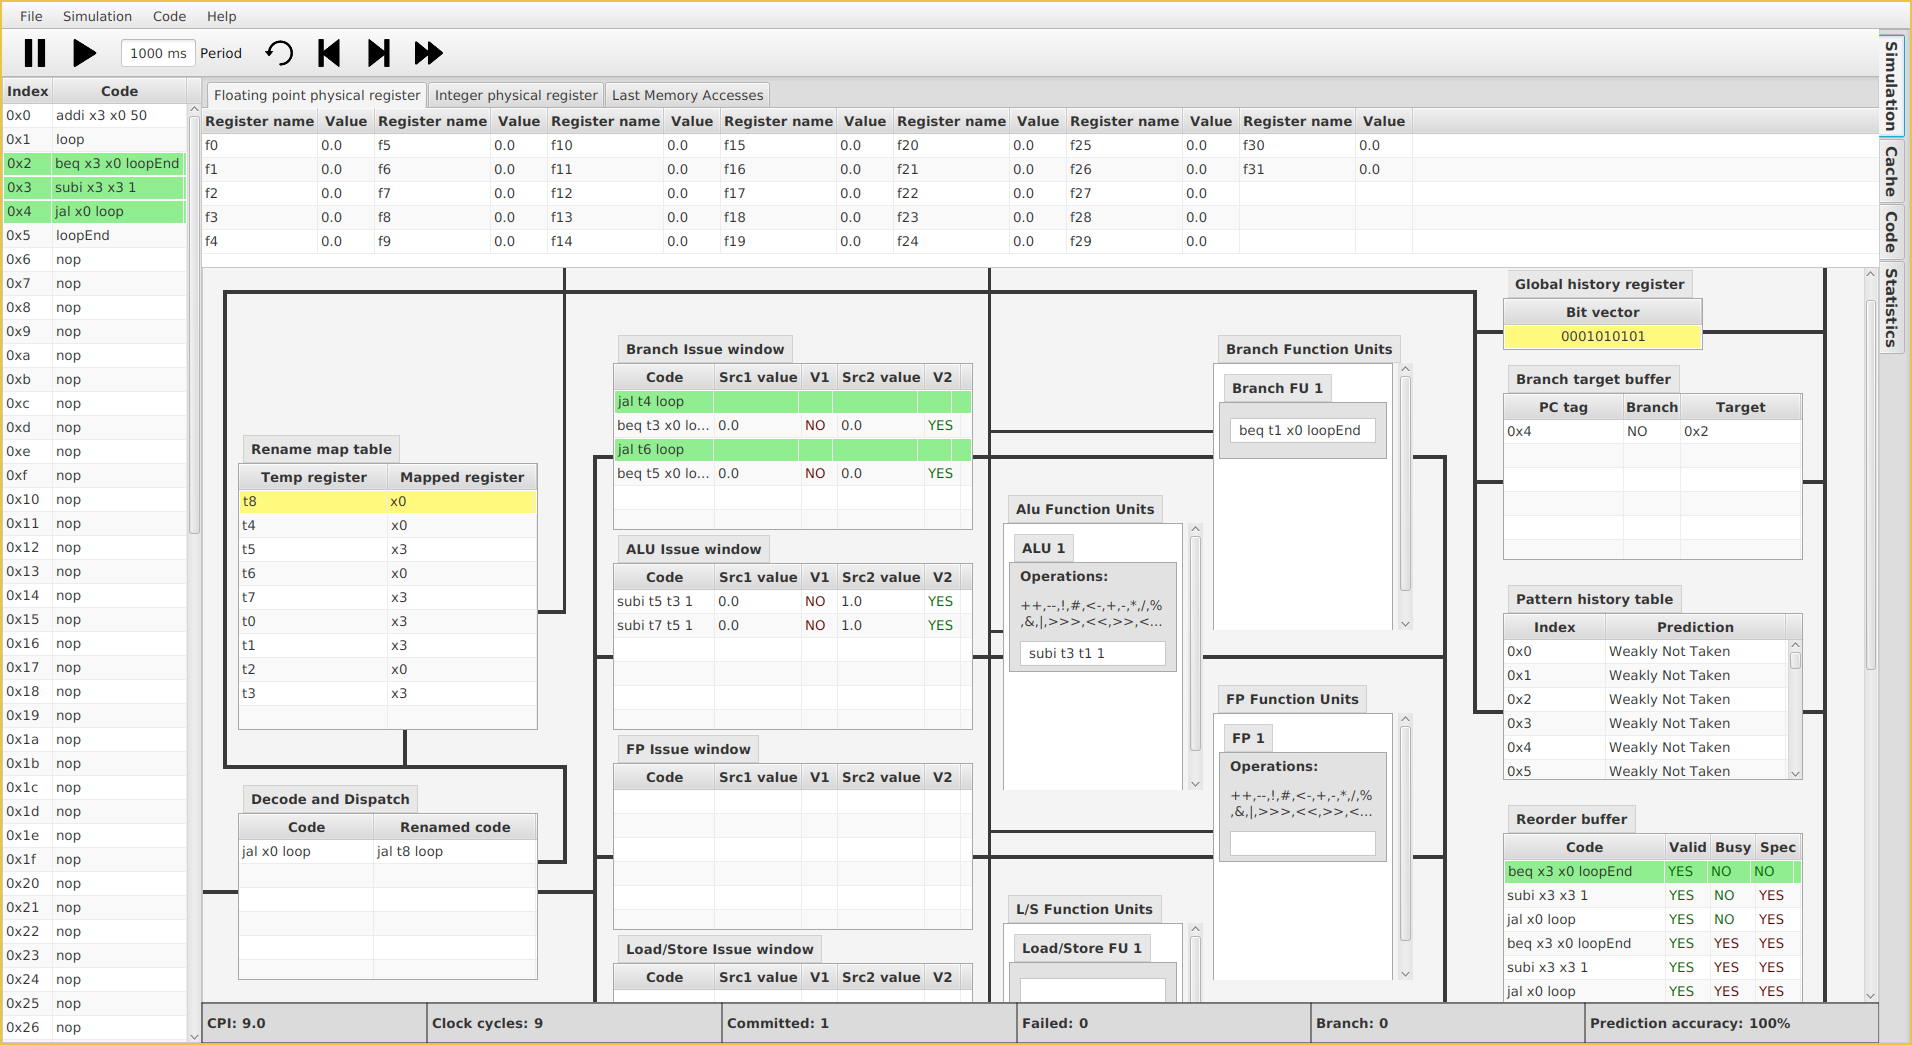
\includegraphics[width=\textwidth]{obrazky-figures/simulating.png}
    \caption{Hlavní okno aplikace v průběhu simulace. Kód, registry a buffery jsou reprezentovány tabulkami. Horní lišta umožňuje spustit celou simulaci, nebo ji postupně krokovat.}
    \label{old_gui}
\end{figure}

\subsection{Statistiky}

Vybrané statistiky jsou zobrazeny v dolní části hlavního simulačního okna (obrázek \ref{old_gui}).
Detailnější pohled poskytuje záložka \emph{Statistics}, kterou je možné vidět na obrázku \ref{stat_window}.
Zde se nachází více číselných statistik a dva grafy vývoje statistik v čase.

\begin{figure}[hbtp]
    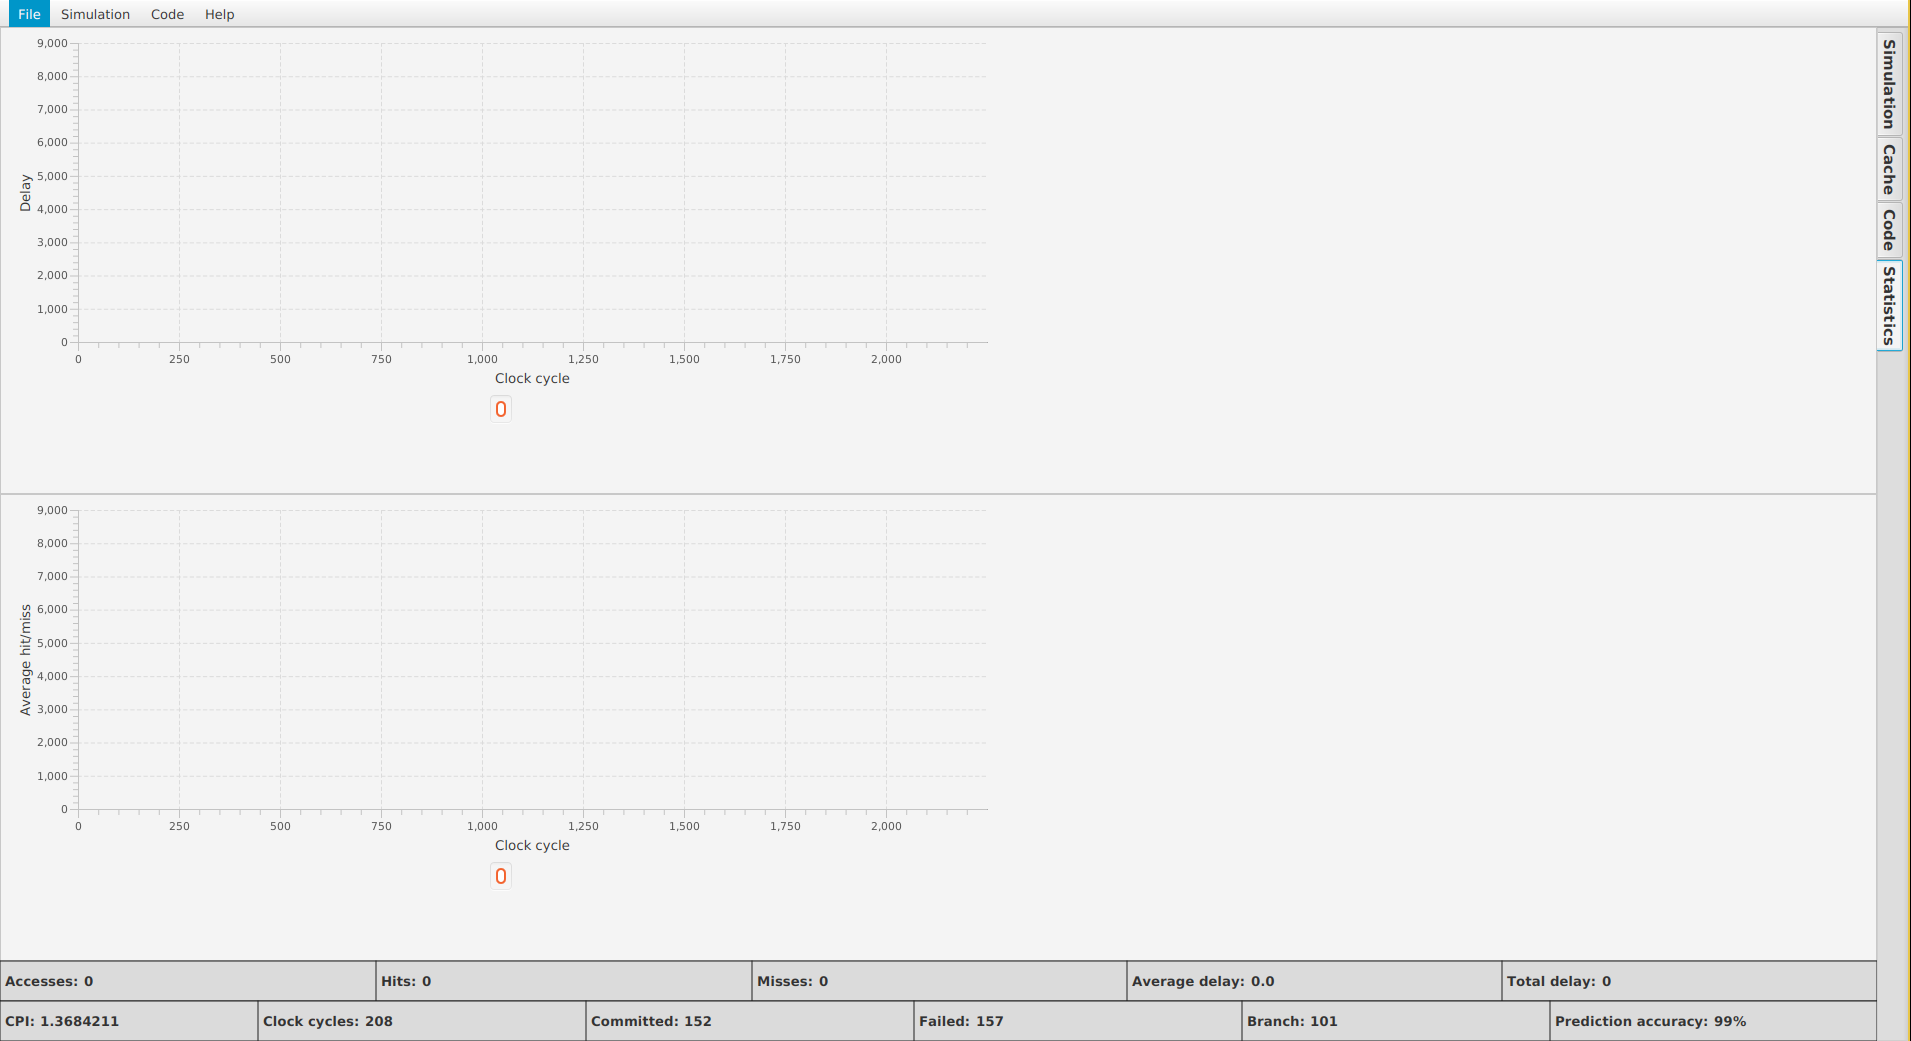
\includegraphics[width=\textwidth]{obrazky-figures/stats.png}
    \caption{Okno pro zobrazení statistik simulace. Ve spodní části se nachází tabulka.}
    \label{stat_window}
\end{figure}

Chybí mi zde více statistik, například instrukční mix (poměr typů instrukcí v kódu), nebo vytíženost funkčních jednotek.
Prezentace statistik také není příliš názorná.

\section{Editor kódu a kompilátor}
\label{inhouse_compiler}

Aplikace umožňuje vytvářet vlastní kódy v assembleru RISC-V, nebo v jazyce C, který je do assembleru následně přeložen.
Kód lze následně přenést do simulátoru.

Editor (na obrázku \ref{code_window}) je praktický.
Zajímavou vlastností je vizualizace vztahu mezi kódem v jazyce C a assemblerem.
Je možné nahrát jeden z mnoha předpřipravených příkladů kódu, což snižuje úsilí nutné k vyzkoušení simulátoru.

\begin{figure}[hbtp]
    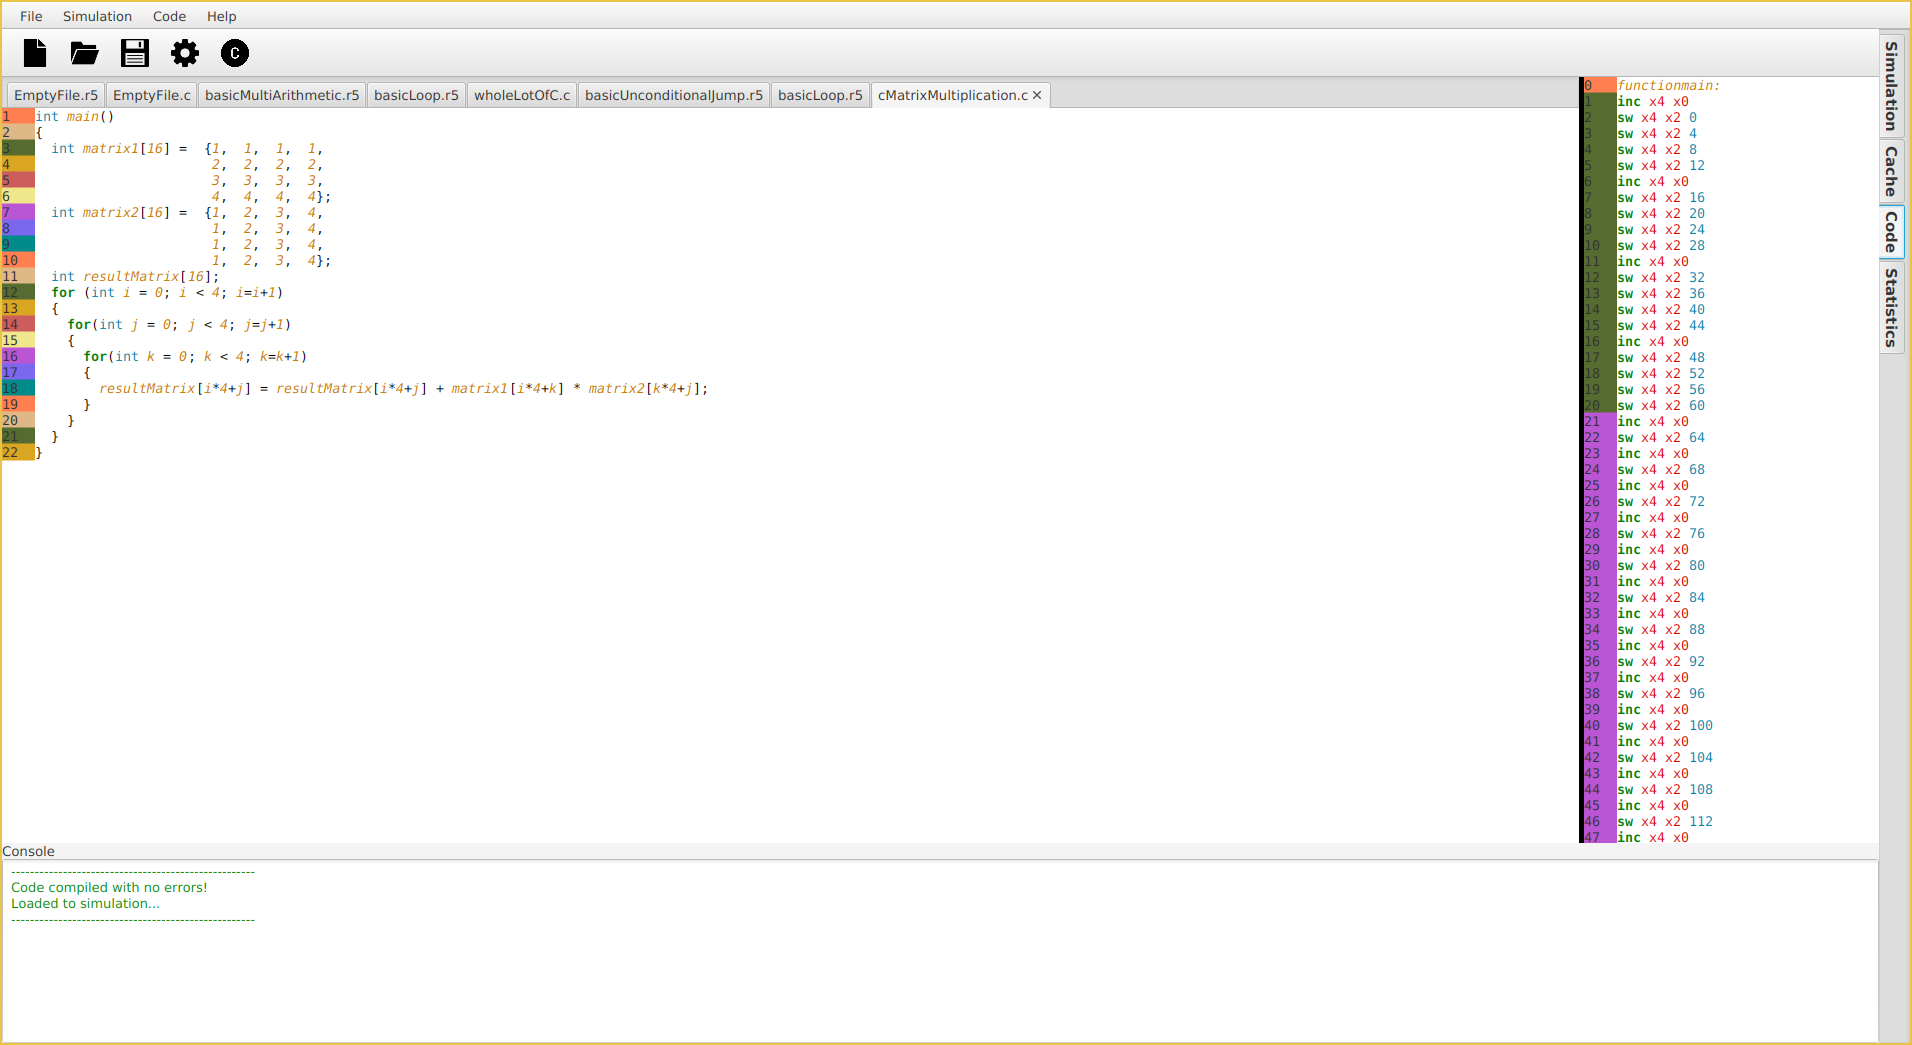
\includegraphics[width=\textwidth]{obrazky-figures/codeeditor.png}
    \caption{Editor kódu zabudovaný v aplikaci. Obsahuje vizuální pomůcky v podobě zvýraznění syntaxe programů a zvýraznění souvisejících částí kódu.}
    \label{code_window}
\end{figure}

Mít překlad plně pod svou kontrolou je velkou výhodou, zejména pokud simulátor nepodporuje všechny instrukce a direktivy, které běžný překladač může vygenerovat, nebo pokud se syntax odchyluje od standardu.
Udržovat vlastní překladač jako součást simulátoru ale považuji za velkou zátěž.
Vyladit všechny chyby je příliš těžké, zpětná vazba kompilátoru v podobě chybových hlášení jsou obecná.
Absence podpory celého standardu C znamená, že kód stažený z internetu často nemusí fungovat.
Uživatel navíc nezná limity překladače, což znesnadňuje práci.

Jediným způsobem jak definovat data je jako jednorozměrné pole v lokální proměnné ve funkci přímo v kódu.
Taková definice dat se navíc přeloží jako série instrukcí \texttt{store} uvnitř těla funkce, což funkci učiní méně čitelnou a zanese šum do běhových statistik programu.

\section{Testování}

Testování je v projektu na skvělé úrovni.
Dobře pokrývá jednotlivé moduly i celkové chování simulátoru, čímž napomáhá snadnějšímu pochopení kódu a ulehčuje refaktorizaci a implementaci nové funkčnosti.

Projekt používá testovací framework JUnit. % https://junit.org/junit5/

Jakub Horký zmiňuje \cite{horkySim}, že implementací nových funkcí musel velkou část testů opravovat.
Z mých experimentů mám podobné zkušenosti, zejména se jedná o holistické testy, které vynucují přesný stav simulace v každém kroku. 

\chapter{Návrh rozšíření simulátoru}

V této kapitole se budu zabývat návrhem rozšíření simulátoru na základě analýzy z předchozí kapitoly.
Navrhnu změnu architektury na serverovou s webovým klientem.
Vylepšení se zaměří na dva aspekty, 1) uživatelské rozhraní a 2) přesnost simulace.

Musí být zachována dobrá rozšiřitelnost a modularita simulátoru.
Implementace by měla v případě budoucího rozšíření povolit nenáročné rozšíření o další část instrukční sady, nebo funkční blok jako například vektorová jednotka.

Při návrhu uživatelského rozhraní jsem se inspiroval původním rozhraním simulátoru Jana Vávry a Jakuba Horkého.
Programátorská rozšíření stavěla na objektové struktuře původního návrhu.

\section{Architektura systému}
% servery, klienti, deployment

Desktopovou aplikaci s grafickým uživatelským rozhraním přetvořím na HTTP server s bezstavovým aplikačním rozhraním využívající HTTP a rozhraním pro lokální práci v příkazové řádce.

HTTP API bude využívat nová klientská webová aplikace.
Ta bude implementovat pouze zobrazení stavu procesoru, editování kódu a konfiguraci simulace.
Vytvořením samostatně stojící prezentační vrstvy získává projekt možnost tyto dva systémy nezávisle nasazovat, udržovat a případně znovu implementovat.

Rozhraní příkazové řádky bude sloužit k automatizovanému spouštění simulací.

\subsection{Webové technologie}

Poskytování uživatelských rozhraní pomocí webového prohlížeče má značné výhody.
Uživatel nemusí plnit složité požadavky na hardwarovou a softwarovou výbavu nutnou k instalaci a spuštění softwaru.
Většina uživatelů již má počítač s moderním webovým prohlížečem a internetové připojení.
% TODO data, zdroj. Kolik procent lidí/počítačů tím disponuje

Vzhledem k původní implementaci v jazyce Java se nabízí možnost implementovat renderování webového uživatelského rozhraní jako modul.
Java k takovým účelům dokonce poskytuje rámcová řešení.
Zachování monolitické povahy simulátoru by bylo výhodou, aplikace ale kvůli požadavkům na názornost a interaktivitu bude vyžadovat značné množství logiky na straně klienta.
% Proč je to výhodné

Ekosystém pro návrh a implementaci front-endových aplikací pomocí JavaScriptu je značně vyspělý.
Z těchto důvodů jsem se rozhodl klientskou aplikaci vyvinout s knihovnou React a frameworkem NextJS.
Při vývoji budu moci využít existující ekosystém pokročilých nástrojů a mnoha knihoven.

\subsection{Aplikační rozhraní}

Simulátor a webová aplikace budou komunikovat pomocí protokolu HTTP aplikačním rozhraním založeným na formátu JSON. 

Stav navracený ze simulátoru by měl být \emph{normalizovaný}.
Simulátor jakožto objektově orientovaný program pracuje s grafem navzájem se odkazujících objektů.
Serializace takového grafu do hloubky způsobí zacyklení.
Navíc, nenormalizovaná data znamenají redundanci v podobě kopií.
Normalizace datových objektů proběhne nahrazením referencí za identifikátory v době serializace.

% Rizika: latence
Možným rizikem je latence serveru při interaktivní simulaci.
Při vývoji a hodnocení budu tuto metriku sledovat a v případě nevyhovujících parametrů implementuji opatření.

\section{Návrh vylepšení simulátoru}

Kromě dále zmíněných konkrétních vylepšení obecně zvýším kvality kódu pomocí refaktorování a dokumentace.
Cílem je mít dobře čitelný, výkonnější a udržitelnější kód.

\subsection{Reprezentace hodnot registrů}

V sekci \ref{repr_reg} jsem uvedl omezení současného systému, který hodnoty registrů reprezentuje v datovém typu \texttt{double}. 

Navrhuji stav registru reprezentovat jako bitové pole.
Interpretace hodnoty bude záviset na právě prováděné instrukci.
Tato reprezentace dovolí přesnou simulaci všech instrukcí, včetně bitových operací.

Bitové pole bude široké 64 bitů, aby bylo připravené pro případné přidání 64 bitové instrukční sady.
V případě implementace vektorových registrů bude nutná malá úprava

Spolu s bitovým polem bude v objektu registru uložena metainformace o významu obsahu, tedy o datovém typu registru. Zdrojem této informace bude popis instrukce, která hodnotu vytvořila.
Tato informace bude soužit pouze k účelům zobrazování hodnoty v GUI a při ladění, při simulaci nebude mít význam.

\subsection{Interpretace instrukcí}

Změny v interpretaci instrukcí úzce souvisí se změnou reprezentace hodnot registrů. Plánuji podporovat celou instrukční sadu RISC-V včetně pseudoinstrukcí. Tento cíl vyžaduje jisté další úpravy.

Navrhuji sjednotit interprety do jedné implementace, která bude dostatečná pro všechny případy užití.

Precedenční interpret nahradím interpretem výrazů v postfixové notaci. Jeho implementace je jednodušší, výrazy nepotřebují závorky a jeho vyjadřovací síla je dostatečná.
Navíc nebude potřeba zvláštního parsování pro operaci přiřazení.

Výpočet některých instrukcí pracuje s hodnotami, které nepatří mezi operandy dané instrukce. Typickým příkladem je použití hodnoty PC při výpočtu adresy skoku. Dalším příkladem je instrukce \texttt{jal}, která načítá hodnotu PC do registru. Další kategorií jsou pseudoinstrukce, které často mají implicitní argumenty. Jako příklad uvedu pseudoinstrukci \texttt{ret}, která odpovídá instrukci \texttt{jalr x0, x1, 0}.

Funkční popis takových instrukcí vyřeším zavedením konceptu proměnných do interpretace. Popis instrukce bude obsahovat všechny argumenty a jejich datové typy. Tyto datové typy budou řídit interpretaci bitů uložených v daných registrech.
Příklad navrhovaného popisu instrukce naleznete na obrázku \ref{code2}.

\begin{figure}[hbtp]
    \begin{lstlisting}[]
       {
        "name": "add",
        "instructionType": "kArithmetic",
        "arguments": [
          {
            "name": "rd",
            "type": "kInt",
            "writeBack": true
          },
          {
            "name": "rs1",
            "type": "kInt"
          },
          {
            "name": "rs2",
            "type": "kInt"
          }
        ],
        "interpretableAs": "\\rs1 \\rs2 + \\rd ="
      },
    \end{lstlisting}
    \caption{Nový popis instrukce \texttt{add} detailně popisuje argumenty a jejich datové typy.}
    \label{code2}
\end{figure}


% default values, pseudoinstructions

\subsection{Rozhraní simulátoru, reprezentace stavu}

Bude odstraněno grafické uživatelské rozhraní, aplikace bude komunikovat bezstavově schématem požadavek/odpověď.
Požadavek bude moct být podán prostřednictvím příkazové řádky (CLI), nebo HTTP dotazu.

Hlavním požadavkem bude dotaz na stav simulace v určitém kroku pro určitou konfiguraci procesoru.
Výstupem bude stav procesoru, statistiky o běhu a ladící výstupy.

Další možné požadavky na simulátor budou:
\begin{itemize}
    \item překlad programu z jazyka C do assembly,
    \item kontrola správnosti programu v assembly,
    \item kontrola správnosti konfigurace CPU pro simulaci.
\end{itemize}

% Požadavky na CLI
Simulace spouštěná z příkazové řádky přijme jako argument konfiguraci procesoru, včetně simulovaného programu.
Výstupem budou především statistiky o dokončeném běhu.
Rozhraní příkazové řádky je určeno primárně pro hromadné vyhodnocování, nebude umožňovat interaktivní simulování, ani překlad programů v jazyce C.

% HTTP
% velikost zpráv, endpointy
HTTP API bude očekávat \texttt{POST} dotazy s parametry předávanými v těle zprávy v jazyce JSON.
Odpovědi budou také v jazyce JSON.
Jazyk JSON jsem zvolil kvůli dobré podpoře jeho zpracování ve webových aplikacích.
Stav procesoru může být objemný, proto plánuji podporovat kódování ZIP, které významně sníží množství dat přenášené po síti.

Dalším problémem je serializace stavu procesoru.
Stav má strukturu obecného grafu objektů s mnoha cykly, které JSON není schopen nativně vyjádřit.
Řešením bude stav normalizovat, převést ho z obecného grafu do stromu a chybějící hrany vyjádřit implicitně identifikátory. 

V současné podobě aplikace nemůže existovat více instancí procesoru.
Stav procesoru bude muset být přesunut do rodičovského objektu, který bude obsahovat reference na všechny své komponenty.

\subsection{Zpětná simulace}

Aby bylo možné realizovat zpětnou simulaci podle současné implementace s bezstavovými dotazy, musel by být stav procesoru přenášen spolu s dotazem.
Logika zpětné simulace je však velmi složitá, výrazně zvětšuje velikost stavu a obsahuje těžko odhalitelné chyby.

Navrhuji jiný přístup.
Stav v libovolném čase $n$ lze vypočítat ze startovací konfigurace, za předpokladu, že je simulace deterministická.
Dotaz tedy nemusí přenášet stav simulace, ale pouze původní konfiguraci.
Veškerá zpětná simulace může být realizována dopřednou simulací z výchozího stavu.

Pro lepší ilustraci uvedu konkrétní příklad.
Předpokládejme situaci, kdy uživatel provozuje interaktivní simulaci a nachází se na 20. taktu.
Pokud uživatel požádá o krok zpět (stav v taktu 19), spustí se simulace z výchozího stavu (stav v taktu 0) a provede se 19 kroků simulace vpřed.

Rizikem tohoto přístupu je latence při interaktivní simulaci -- délka výpočtu následujícího stavu bude růst lineárně s aktuální pozicí v simulaci, protože celá simulace musí proběhnout znovu.
V případě, že odpověď serveru nebude spolehlivě dosahovat interaktivní rychlosti, je možné implementovat cache rozpočítaných simulací.
% Obsloužení dotazu bude mít stále konstantní cenu.

\subsection{Přesnost simulace}
% labels - návěstí, instruction set, tests, Expression

Mým cílem je implementovat všechny instrukce základní instrukční sady RV32I a rozšíření M a F.
Výjimkou budou instrukce pro komunikaci s jádrem, protože není implementovaný privilegovaný režim ani přepínání kontextu.
Implementuji i velkou část pseudoinstrukcí.

Každá z instrukcí bude přesně odpovídat specifikaci.
Instrukce programu ale budou i nadále vnitřně reprezentovány polem objektů, nebudou zavedeny a čteny z paměti.

Skokové a paměťové operace pracují s adresami návěstí.
V současné implementaci ale hodnota návěstí představuje index do pole instrukcí.
Návěstím je nutné přiřadit reálné adresy, aby hodnoty odpovídaly očekávání překladače a aby mohly návěstí ukazovat na staticky alokovaná pole a konstanty (více v sekci \ref{memloader}).

\subsection{Konfigurace simulace}

Stávající konfigurace je převážně vyhovující.
Hlavní změnou konfigurace jádra bude zjednodušení konfigurace ALU.
Místo seznamu operací si uživatel bude moci vybrat jednu nebo více z pěti funkcionalit: sčítací operace, bitové operace, násobení, dělení a speciální funkce.

V GUI přidám detailní popisy ke každé možnosti konfigurace, aby bylo zřejmé jaký efekt má na simulaci.
Přibude i validace vstupů s dobrou zpětnou vazbou pro uživatele.

Novou funkcí bude definice paměťových míst přímo v konfiguraci.
Je užitečné sledovat běh algoritmů na určitých datech, například některá chování cache se projeví až při práci s větším množstvím (kilobajty) dat
Navrhuji přidat možnost pohodlně definovat větší datové vstupy položkami v aplikačním dotazu (tedy jinou cestou, než direktivami v kódu).
Paměťové místo bude definované svým názvem, datovým typem, požadavkem na zarovnání v paměti a seznamem číselných hodnot.

\subsection{Kompilace programů v jazyce C}

Překladače jsou jedním z nejkomplexnějších problémů oblasti informatiky.
Proto by bylo vhodné použít hotové řešení.

Vybral jsem si překladač \emph{GCC}, jeden z nejpoužívanějších překladačů pro jazyk C.
Poskytuje užitečná chybová hlášení, je dobře otestovaný, rychlý a implementuje veškeré potřebné funkce jazyka C.

GCC má mnoho funkcí a obsáhlou dokumentaci.
Plánuji uživatelům zpřístupnit ovládání optimalizací.
Bude také možné si vyzkoušet efekt direktiv jako \texttt{\#pragma unroll}. 

Tento překladač podporuje \emph{cross-compilation}, kompilaci pro jinou architekturu, než ta, na kterém je překladač spouštěn.

Překladač bude front-endové aplikaci zpřístupněn jako součást simulačního API. 
Serverová aplikace bude binární program GCC spouštět přes shell se zvolenými přepínači.
Řetězec s programem bude poslán na jeho standardní vstup, z výstupu bude přečten assembler pro RISC-V.
Chybová hlášení budou předána zpět uživateli webového editoru.

Překladač generuje jiný kód, než jaký v současnosti překladač očekává.
Změny, které musím implementovat zahrnují:
\begin{itemize}
    \item změnu syntaxe (viz sekce \ref{riscvSyntax}),
    \item přidání podpory pro aliasy registrů,
    \item implementaci všech instrukcí, které překladač může generovat,
    \item alokaci zásobníku volání (viz sekce \ref{memloader})
    \item zastavení simulace při vyprázdnění zásobníku volání,
    \item filtrování ladících symbolů a nepoužitých direktiv.
\end{itemize}

\subsection{Syntax programů v asembleru RISC-V}
\label{riscvSyntax}

Protože plánuji používat klasický překladač, budu muset simulátor upravit tak, aby přijímal tradiční assembler RISC-V.
To znamená především:
\begin{itemize}
    \item přidání oddělovačů mezi parametry (čárky a závorky),
    \item parsování direktiv (například \texttt{.word}),
    \item implicitní paramtery (pro pseudoinstrukce).
\end{itemize}

\subsection{Sběr statistik o běhu}
\label{statsCollection}

Sběr statistik bude detailnější.
Zaměřím se jak na globální statistiky, tak i statistiky jednotlivých instrukcí.

Konkrétní návrhy nových statistik:
\begin{itemize}
    \item statický a dynamický instrukční mix,
    \item vytíženost každé funkční jednotky,
    \item počty provedení každé instrukce,
    \item nové charakteristiky (FLOPS, aritmetická intenzita).
\end{itemize}

\subsection{Zavádění dat do paměti procesu}
\label{memloader}

Data definovaná v konfiguraci i v assembleru direktivami\footnote{Jako příklad, \texttt{A: .word 1,2,3,4} definuje pole \texttt{A} o čtyřech 32 bitových prvcích.} musí být staticky alokována v hlavní paměti procesoru.
Alokace proběhne podle požadavků na datový typ a \emph{zarovnání}.

Program v jazyce C bude přeložen do direktiv.
Tímto způsobem bude možné alokovat globální proměnné, včetně struktur a řetězců definovaných v jazyce C.

Kód s pamětí následně bude pracovat pomocí návěští (labels), která do této doby byla používaná pouze pro adresy skoků.
Hodnoty návěští budou představovat ukazatele na tato pole.
% návěští nebo label nebo?

% alokace zásobníku volání
ABI používané překladačem počítá s alokovaným zásobníkem volání.
Proto inicializace paměti musí vyhradit místo pro zásobník a zapsat ukazatel do registru \texttt{x2} (neboli \texttt{sp}).

Příklad rozložení zásobníku volání a dvou polí se zarovnáním lze vidět na obrázku \ref{memlayout_schema}.

\begin{figure}[hbtp]
\centering
    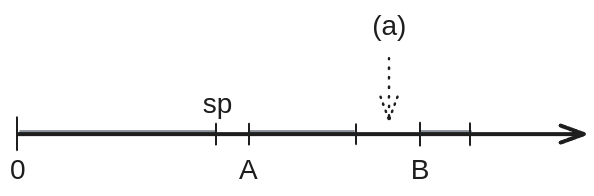
\includegraphics[width=13cm]{obrazky-figures/memlayout.png}
    \caption{Schéma rozložení dat v paměti procesoru. Počáteční adresy jsou vyhrazeny pro zásobník volání. Následně jsou alokována jednotlivá pole. Prázdné místo mezi bloky (zvýrazněno jako \emph{(a)} může vznikat požadavkem na zarovnání počátku pole v paměti.} 
    \label{memlayout_schema}
\end{figure}

\subsection{Ladící výstupy v průběhu simulace}

\section{Návrh webové aplikace}
% Rozhraní simulátoru
% GUI

Rozhraní bude v anglickém jazyce.
Cílovou skupinou pro aplikaci jsou studenti vysokoškolského kurzu AVS, angličtina je pro studium předpokladem.
Angličtina také dovolí projekt používat v mezinárodním prostředí. 
Vícejazyčná podpora vyžaduje mnoho práce, i za použití internacionalizačních knihoven jako \texttt{i18next}.

Obrázek \ref{main_view_design} schématicky naznačuje možný vzhled hlavního simulačního okna.
Myšlenka současného rozhraní se nemění -- jednotlivé bloky procesoru jsou reprezentovány odpovídajícími komponenty, související bloky jsou spojeny čarami, které představují datové cesty procesoru.

\begin{figure}[ht]
    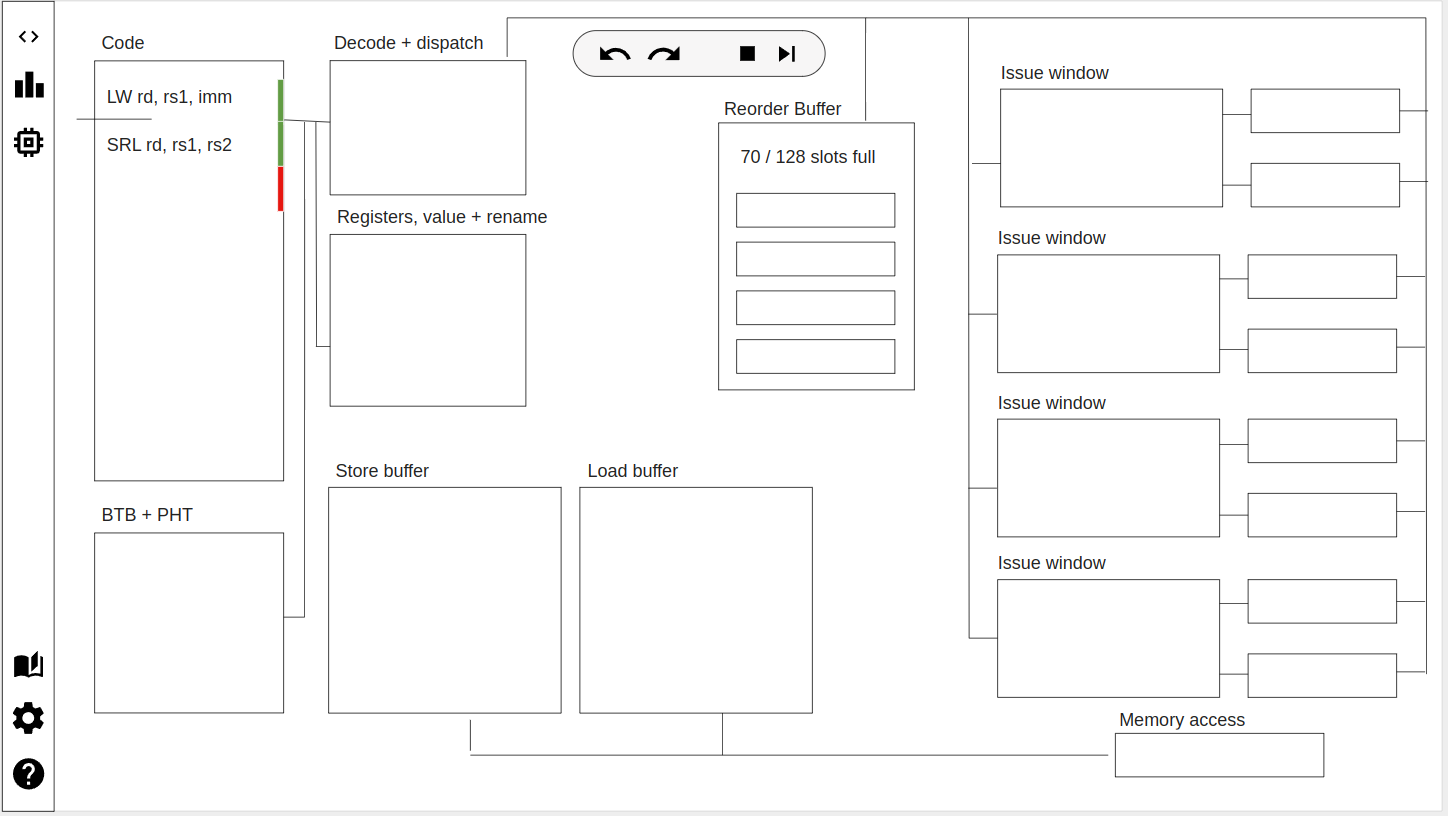
\includegraphics[width=\textwidth]{obrazky-figures/main_view_design.png}
    \caption{Schéma grafické reprezentace stavu simulace. Na levé straně jsou odkazy na ostatní okna aplikace.}
    \label{main_view_design}
\end{figure}

Bloky simulace i jednotlivé instrukce by měly mít možnost detailnějšího náhledu.
Ten by kromě detailních dat měl poskytnout odkaz na dokumentaci dané instrukce nebo bloku.

Další část, která se příliš nezmění, bude ovládání simulace.
V horní části obrazovky budou k dispozici tlačítka pro krokování a dokončení simulace.
Pro větší komfort a dostupnost bude možné simulaci ovládat klávesnicí.

\subsection{Editor kódu}
% Co je pro uživatele důležité - feedback

Záložka pro editování kódu bude umožňovat vytváření a upravování kódu v jazyce C a v assembleru RISC-V.

Cílem je při psaní kódu poskytnout dobrou zpětnou vazbu.
Editor bude využívat API simulátoru pro překlad a kontrolu kódu z jazyka C do assembleru.
Syntax a případné chyby v kódu budou v textovém poli znázorněny.
Přeložený kód bude barevně vizualizovat vztah řádků původního a přeloženého programu podobným způsobem. 

K dispozici bude několik příkladů kódů, jak pro jazyk C tak Assembler.
Příklady umožní novým uživatelům rychle začít se simulátorem experimentovat.

\subsection{Výukové materiály}
% Texty vysvětlující RISC-V, jednotlivé bloky procesoru

Cílovými uživateli aplikace budou studenti kurzu AVS.
AVS se nezaměřuje na konkrétní instrukční sadu, proto bude pohodlné poskytnout základní informace o sadě RISC-V v podobě vysvětlujícího textu a tabulek.
Popis může používat odborné termíny a může se opřít o znalosti již nabyté v průběhu předmětu AVS.

\subsection{Konfigurační stránka}
% uložit konfigurace

Konfigurace obsahuje mnoho položek, proto její vytvoření může zabrat čas a bránit od plynulého používání aplikace.
Aplikace by proto měla poskytnout rozumný výchozí profil, který by byl vyhovující pro širokou škálu experimentů.

Z vlastní zkušenosti při experimentech s existující konfigurací simulátoru vím, že může být obtížné představit si pod názvem konfiguračního pole jeho efekt na simulaci.
Budu klást důraz na kvalitu jmen a popisů jednotlivých polí formulářů.

Všechny vytvořené konfigurace budou uloženy lokálně v úložišti prohlížeče a budou perzistovány napříč sezeními.
Tímto návrhem se vyhnu nutnosti spravovat uživatele v databázi.
Alternativním přístupem by mohlo být použití autentizace a uložení dat aplikace externí službou.
Lokální úložiště je však dostatečnou a nekomplikovanou variantou.
% todo jak je na tom localstorage a gdpr, cookies zákony 

\subsubsection{Definice dat}

Pro definici simulačních dat (paměti) bude vyhrazena zvláštní sekce konfigurace. 
Uživatel bude moci definovat libovolný počet pojmenovaných paměťových lokací, na které se tímto jménem bude odkazovat v kódu.

Počet prvků paměťového místa bude konfigurovatelný.
Hodnoty jednotlivých prvků budou inicializovány jedním ze tří způsobů:
\begin{enumerate}
    \item kopírováním konstanty,
    \item náhodnými daty,
    \item daty ze souboru CSV.
\end{enumerate}

\subsection{Prezentace statistik}

V průběhu simulace bude možné nahlédnout na stránku se statistikami.
Zde budou prezentovány běhové statistiky popsané v sekci \ref{statsCollection}.
Stránka poskytne přesná tabulková data i jejich vizualizaci, například teplotní mapou a grafy. 

Statistiky týkající se konkrétních bloků budou také přístupné z jejich detailního pohledu ve "vyskakovacím okně". 

\section{Případy užití a kritéria příjmutí}
% Jak to bude testováno
% load testing
%todo

Je plánováno aplikaci využít pro výuku předmětu AVS na FIT VUT v Brně.
Aplikace bude proto mít potenciálně stovky uživatelů.
Studenty kurzu AVS bych řadil mezi zkušené uživatele webových aplikací, nicméně bude klíčové klást důraz na intuitivnost, spolehlivost, dostupnost a výkon.

Spolehlivost aplikace ověřím dobrým automatizovaným testováním na úrovni modulů i celku.
Uživatelské rozhraní budu testovat převážně manuálně, ve dvou fázích.
Nejdříve budu testovat aplikaci v průběhu vývoje.
Ověřím funkčnost na několika populárních internetových prohlížečích.

Později aplikaci nechám vyzkoušet několika studentům informatiky.
Při testování budu sledovat jejich práci a sbírat zpětnou vazbu.
Zpětnou vazbu využiji ke zlepšení aplikace.
Dalším zdrojem zpětné vazby je vedoucí mé práce, pan docent Jaroš, se kterým vývoj aplikace pravidelně konzultuji. 

Z pohledu implementace je cílem co nejvyšší bezúdržbovost s dostatečnou dokumentací pro případné drobné opravy.
Kód také může někdo v budoucnu (stejně jako já nyní) rozšiřovat.
Klíčová bude především kvalita podpůrných dokumentů a řádně okomentovaný kód s výstižnými jmény.

Zvážen bude i výkon aplikace.
Cílem je interaktivní simulace, proto by server měl na dotazy odpovídat do 100\,ms.
Zároveň by mělo být možné obsluhovat stovky uživatelů současně.
Splnění tohoto cíle ověřím zátěžovými testy.

Program bude pravděpodobně promítán na plátně během výuky.
Proto budu brát ohled na kontrast, možnost libovolného zvětšení prezentace simulace a na její správné škálování.

\chapter{Závěr}
% pro SEP

V této semestrální práci jsem prozkoumal některé známé metody efektivní implementace superskalárních procesorů.
Konkrétněji jsem se zaměřil na instrukční sadu RISC-V, kterou simulátor využívá.
Také jsem uvedl teorií implementace webových aplikací s přihlédnutím k návrhu uživatelských rozhraní.

Provedl jsem důkladnou analýzu stávajícího simulátoru, zhodnotil jeho klady i nedostatky a navrhl jsem mnoho zlepšení, jak z pohledu implementace simulace, tak použitelnosti jeho rozhraní.

Aplikace je v současné podobě provozuschopná.
Na webové stránce je možné provozovat interaktivní simulaci, měnit konfiguraci, editovat kód a prohlížet statistiky o simulaci.
Příloha \ref{prevzanaPrace} uvádí tabulku s přehledem jednotlivých modulů aplikace a můj přínos.

Další vývoj bude spočívat v implementaci chybějících částí systému.
Nejdůležitější chybějící funkcí je rozhraní příkazové řádky.
Další úkoly na letní část práce jsou implementace ladících výstupů, implementace chybějících prvků uživatelského rozhraní simulátoru, vylepšení testů a oprava chyb v logice a optimalizace výkonu.
V posledních týdnech proběhne uživatelské testování, na základě kterého provedu úpravy.
Výsledky testování také vyhodnotím.

    
\chapter{Implementace rozšíření simulátoru}
\label{Implementacerozs}
% Java

Tato kapitola se zaměřuje na konkrétní postup implementace úprav a rozšíření simulátoru, které byly popsány v sekci \ref{rozsireniJava}.
Podrobněji bude popsána hlavní simulační smyčka, zpracování assembleru a implementace serverového rozhraní.

\section{Refaktorizace}
% cache, registry, volání bloků, prediktory, labels
% přehled změn popsaných v této kapitole

Refaktorizace kódu byla prvním implementačním úkolem.
Probíhala zároveň s~analýzou a návrhem a sloužila jako příprava k~pozdějšímu přidávání nových funkcí.
Úpravy v~této fázi byly menšího rozsahu, především se jednalo o~lokální změny v~rámci funkcí a přidávání komentářů.
V~druhé fázi přišly na řadu větší celky, včetně jejich rozhraní.
Důvodem k~zásahu bylo buď zvýšení čitelnosti, nové požadavky na modul, nebo potřeba změnit reprezentaci pro snadnou serializaci (a následné zobrazení na webu).

Určit hranici mezi refaktorováním a novou implementací není jednoduché.
Většina modulů se změnila zásadním způsobem, včetně způsobu interakce mezi moduly.
Příloha \ref{prevzanaPrace} uvádí tabulku s~přehledem jednotlivých modulů aplikace a můj přínos.

% SimCodeModel - zrušena dědičnost, exceptions, sloučení se stavem ROB (předělání renamedLine)
Třída \texttt{SimCodeModel} představující instrukci v~systému obsáhla stavové informace z~ROB, nově také nese informace o~vyvolané výjimce a lépe strukturované informace o~skoku a své pozici v~kódu.

% Load/Store - transakce
% TODO jak vypadala hlavní paměť dřív?
Paměťový modul (hlavní paměť a cache) zaznamenal významné změny, ale princip fungování zůstal stejný.
Tyto bloky nyní pracují v~\emph{transakčním režimu}.
Funkční bloky, které požadují data z~paměti generují nový objekt představující transakci.
Při registraci správa paměti tento objekt vyplní údajem o~délce vybavení transakce.
Transakce umožňují lehkou konfiguraci doby vybavení z~paměti, jsou kompatibilní s~vypláchnutím linky a obsahují metadata, která jsou zajímavá při interaktivní simulaci.

Není možné zmínit každé vylepšení.
Jako příklad menších úprav uvedu změnu vyjádření prediktorů skoků.
Původní návrh využíval dědičnosti tříd.
Implementace byla zredukována na jedinou třídu \texttt{BitPredictor}, kterou je možné parametrizovat.
Výsledkem bylo zjednodušení kódu (4 původní třídy byly sloučeny do jedné univerzální) a lepší kompatibilita se serializací do JSONu.

\subsection{Registry}
% Reference a lineární prohledávání registrového pole podle stringového jména
% Ukládání hodnoty jako double
% Držení stavu registru v jiné struktuře

Problémem jak z~výkonnostního tak z~návrhového hlediska byla práce s~registry.
Instrukce držely reference na registry jako řetězce s~jejich názvy (např. \texttt{\uv{x5}}, \texttt{\uv{tg24}}).
Při \emph{každém} přístupu k~hodnotě registru bylo nutné provést lineární vyhledávání nad celým registrovým polem, tedy nad stovkami registrů a pro každý prvek muselo proběhnout porovnání s~hledaným řetězcem.
Metadata registru byla navíc udržována v~jiné datové struktuře, takže bylo nutné provést druhé vyhledání.
Také bylo nutné tyto struktury udržovat synchronizované.

Reference v~podobě řetězců jsem nahradil opravdovými \emph{referencemi} na objekt.
Nyní přístup k~registru odpovídá následování ukazatele, což je mnohem efektivnější operace.
Registr je vyhledáván pouze jednou při inicializaci programu a jednou při přejmenování instrukce.

Nový návrh objektu \texttt{RegisterModel} obsahuje svůj datový typ a stav alokace.
Hodnota již není reprezentována datovým typem \texttt{double}, ale novým objektem třídy \texttt{Register\-Data\-Container}, která dokáže reprezentovat jak celá čísla, tak i čísla ve formátu plovoucí desetinné čárky.
Objekt zapouzdřuje pole 64 bitů v~podobě proměnné typu \texttt{long}, ke kterému nabízí jak přímý přístup, tak interpretovaný přístup.

Registr také obsahuje všechny informace nutné k~přejmenování.
Všechny registry mají počet referencí, architekturní registry využívají seznam přejmenování a spekulativní registry obsahují odkaz na odpovídající architekturní registr.

Díky detailním metadatům je možné registry v~interaktivní simulaci detailně zkoumat.

Další souvislostí je, že díky odkazovatelnosti na objekty \texttt{RegisterDataContainer} nemusí být hodnoty kopírovány mezi buffery (například v~blocích \texttt{issue} a \texttt{load buffer}). 

\section{Simulace}
\label{implSimulace}

Významnou změnou je nový způsob zpětné simulace navržené v~sekci \ref{backSimNewDesign}.
Bloky nyní neobsahují logiku pro zpětnou simulaci ani datové struktury, které byly pro zpětný chod nutné.
Kód se stal významně jednodušším, protože operace nyní nemusí být reverzibilní.

Původní implementace simulační logiky používala návrhové vzory jako \emph{Singleton} a \emph{Dependency Injection}, které komplikovaly vytváření instancí procesoru.
V~aplikaci navíc nemohlo souběžně existovat více instancí procesoru, což znemožnilo implementaci obsluhy dotazů na server.
Tento přístup také komplikoval testování procesoru jako celku.

Zapouzdřil jsem proto všechny bloky procesoru a jejich inicializaci do třídy \texttt{Cpu}.
Rozhraní pro vykonání simulace se stalo významně jednodušším.
Příklad provedení simulace je uveden v~kódu \ref{cpuApi}.
Po volání \texttt{execute} je objekt \texttt{cpu} ve stavu na konci simulace.
Tento stav je možné zkoumat v~rámci testu, nebo prezentovat uživateli.

\begin{lstlisting}[caption={Příklad spuštění simulace s~výchozí konfigurací a vlastním kódem.},captionpos=b,label=cpuApi]
SimulationConfig config = SimulationConfig.getDefaultConfiguration();
config.code = "addi x8, x8, 5";
Cpu cpu = new Cpu(config);
cpu.execute(false);
\end{lstlisting}

%step
Funkce \texttt{execute} je funkcí pro pohodlí při testování.
Pro potřeby interaktivní simulace existuje metoda \texttt{simulateState(targetTick)}, která ve smyčce volá \texttt{step}.
Detailnější popis rozhraní třídy Cpu je uveden v~sekci \ref{simLoop}.

% determinismus
Simulace je deterministická.
Determinismus je v~místech, kde se pracuje s~náhodou, docílen inicializací pseudonáhodného generátoru do stejného výchozího stavu.

\subsection{Inicializace a Hlavní smyčka simulace}
\label{simLoop}
% Vstupní bod, konfigurace, class Cpu init, zásobník (i zastavení simulace)
% step(), simEnded()
% Komunikace bloků, jejich pořadí

Inicializace objektu procesoru sestává z~následujících kroků:
\begin{enumerate}
    \item validace konfigurace,
    \item načtení popisu instrukcí a registrů,
    \item inicializace podpůrných objektů (statistiky a manažery),
    \item parsování assembleru,
    \item inicializace paměti (data, zásobník),
    \item vytvoření bloků procesoru a jejich vzájemných referencí,
    \item inicializace hodnot registrů,
    \item nastavení PC na počátek programu.
\end{enumerate}

Konfigurace procesoru probíhá při fázi inicializace.
Jedná se o~velikosti pamětí, zpoždění bloků, prováděný program a data.
Kompletní výčet se nachází v~příloze \ref{cpuConfigAppendice}.

Dalším krokem je získání popisů instrukcí a nové kopie registrového pole.
Tato data jsou načtena ze souborů při startu aplikace a cachována v~paměti.

% memory
Inicializace paměti na začátku paměťového prostoru vyhrazuje konfigurovatelné množství paměti pro zásobník volání.
Do vyšších adres se poté kopírují data definovaných objektů (polí, konstant a struktur).
Alokace jsou zarovnané podle požadavků.

% entryPoint
Vstupním bodem programu může být podle konfigurace libovolné návěstí nebo adresa.
Na požadovanou hodnotu je nastaven registr PC bloku Fetch.
Samotná simulace spočívá v~opakovaném volání funkce \texttt{step}, která představuje jeden takt procesoru.
Simulace probíhá buď do konce programu pro CLI, nebo do požadovaného taktu v~případě interaktivní simulace.

% todo mediator? https://refactoring.guru/design-patterns/mediator
Jeden takt je simulován sekvenčním voláním všech bloků procesoru.
Pořadí bloků bylo oproti původnímu řešení změněno.
Důvodem byly změny ve vydávání instrukcí do funkčních jednotek a změna paměťového systému.
V~případě funkčních jednotek byla simulace kroku rozdělena do dvou funkcí volaných v~různý čas v~rámci taktu, aby bylo možné nasimulovat dokončení jedné instrukce a načtení nové v~rámci jednoho taktu.
% teď bych podobně rozdělil více bloků, ale oh well, future work

% simStatus
Ve funkci \texttt{simStatus} probíhá při každém cyklu kontrola, jestli má simulace pokračovat, nebo se ukončit.
Simulace může být ukončena potvrzením výjimky, limitní podmínkou proti zacyklení, nebo řádným ukončením programu.

Simulátor podporuje dva režimy vykonávání programů.
V~prvním případě je simulace ukončena jakmile je linka prázdná a PC je za poslední instrukcí programu.
Tento režim je vhodný pro jednoduché ukázky bez zásobníku volání.

Druhým režimem je režim se \emph{zásobníkem volání}.
Registr \texttt{sp} je inicializován na adresu vrcholu zásobníku a registr \texttt{ra} je inicializován na 
speciální adresu.
Jakmile ROB potvrdí skok na tuto adresu, vysílá signál a simulace je ukončena.
Tento mechanismus zastupuje operační systém a runtime, který by typicky vstupní funkci obalil kódem pro ukončení procesu.

\subsection{Bloky procesoru}
% Detaily k blokům
% menší provázanost

Každý blok je inicializován konstruktorem s~relevantními parametry konfigurace a referencemi na ostatní bloky.

Bloky mezi sebou komunikují přímými referencemi.
Atributy jsou z~velké části privátní, kód ale obsahuje velké množství metod, které tyto atributy přímo nastavují.
Tím je narušeno zapouzdření.
Byla snaha zredukovat počet referencí, aby se zjednodušil model komunikace a bylo jednodušší o~systému uvažovat.

Rozhraní mezi řídící třídou \texttt{Cpu} a každým blokem je funkce \texttt{simulate(int cycle)}.
Výjimku tvoří funkční jednotky, jejichž logika je rozdělena do dvou fází -- dokončení a začátek vykonávání instrukce.
Rozdělení řeší problém opuštění a vstupu instrukcí do funkční jednotky během stejného taktu.
V rámci budoucí práce navrhuji prozkoumat rozdělení simulace více bloků do několika fází, což by mohlo zjednodušit logiku.

Číslo cyklu je nyní předáváno při volání simulate.
Nové rozhraní preferuji před původním řešením, kde si každý blok udržoval vlastní čítač.

Funkční jednotky zůstaly neřetězené.
Implementace zřetězení by mohla být předmětem budoucí práce, protože zřetězené linky odpovídají reálným implementacím funkčních jednotek.

\subsection{Běhové statistiky}
% sběr statistik, celkové a pro instrukci
% log?

Stav simulace obsahuje centrální objekt průběžně shromažďující statistiky.
Jednotlivé statistiky se vztahují buď k~celému procesoru, nebo ke konkrétní instrukci.
Celý výčet statistik je k~dispozici v~příloze \ref{statsAppend}.

%aggreg
Na základě statistických dat je možné vyhodnotit úspěšnost spekulativního počítání.
Je k~dispozici počet vypláchnutí linky a úspěšnost predikce skoků.
Kromě absolutních čísel jsou spočítány i některé metriky (IPC, FLOPS, cache hit rate).

Velká část statistik sleduje paměťový systém.
Sledují se počty přístupů do paměti, počet zásahů do cache (\emph{cache hits}, viz sekce \ref{cache}) a množství čtených a zapsaných dat.
Přístupy a úspěšnost vyhledání v~cache se evidují i pro jednotlivé instrukce.

\section{Instrukce a jejich interpretace}
% syntax, interpretace
% loading from JSON

% Instrukční sada, hierarchie (functionmodel, input, simcodemodel)
Objektový návrh instrukcí založený na dědičnosti a lineárním vyhledávání v~seznamu instrukcí jsem nahradil \emph{kompozicí}.
Instance instrukce v~procesoru se přímo odkazuje na instrukci v~programu, která se zase přímo odkazuje na obecný popis konkrétní instrukce.
% todo ilustrace / uml diagram

Původní popis instrukce uvedený v~sekci \ref{interpret} jsem rozšířil podle návrhu v~sekci \ref{instructionNewDesign}, aby byl více explicitní a dokázal vyjádřit význam všech implementovaných instrukcí.
Implicitní argumenty instrukcí jako \texttt{call} a \texttt{ret} jsou nyní podporovány.

% interpretableAs
Vykonání výrazu instrukce probíhá v~nové třídě \texttt{Expression}, která implementuje jednoduchý interpret založený na zásobníku.
Několik ukázek je uvedeno v~tabulce \ref{interpreTable}.
Proměnná značená zpětným lomítkem přidá na zásobník hodnotu, operand vybere operandy ze zásobníku a výsledek vloží zpět na zásobník.
Instrukce \texttt{jal} ukazuje možnost použití \texttt{pc} při interpretaci.
Dvojtečka rozděluje podvýrazy u~paměťových a skokových instrukcí.
U paměťových operací je prvním podvýrazem akce (load/store), druhým podvýrazem je adresa.
U skokových operací je prvním podvýrazem adresa skoku a druhým podvýrazem je podmínka skoku.

Výstup z~výrazu je dvojí.
Prvním výstupem je hodnota, která po provedení interpretace zůstane v~zásobníku.
Tohoto mechanismu využívají výrazy pro výpočet adresy skoku nebo podmínky skoku.
Druhým výstupem je přiřazení do proměnné ve výrazu.
Binární operátor \texttt{=} ve výrazu má vedlejší efekt, který hodnotu propíše i do registru.

\begin{table}[]
\begin{tabular}{|l|p{5cm}|p{5cm}|}
\hline
Instrukce            & Výraz                                                                                                                  & Význam                                                   \\ \hline\hline
\texttt{add rd, rs1, rs2}     & \texttt{\textbackslash{}rs1 \textbackslash{}rs2 + \textbackslash{}rd =}                                                         & Sčítání                                                  \\ \hline
\texttt{fmin.s rd, rs1, rs2}  & \texttt{\textbackslash{}rs1 \textbackslash{}rs2 \textbackslash{}rs1 \textbackslash{}rs2 \textgreater\ pick \textbackslash{}rd =} & Přiřazení menšího z~operandů do \texttt{rd}                       \\ \hline
\texttt{lb rd, imm(rs1)}      & \texttt{load:8:\textbackslash{}rs1 \textbackslash{}imm +}                                                                     & Načtení 8 bitů z~adresy \texttt{rs1+imm}                          \\ \hline
\texttt{fsgnj.s rd, rs1, rs2} & \texttt{\textbackslash{}rs1 bits 0x7fffffff \& \textbackslash{}rs2 bits 0x80000000 \& | float \textbackslash{}rd =}             & Spojení hodnoty v~plovoucí čárce \texttt{rs1} a znaménko z~\texttt{rs2}    \\ \hline
\texttt{jal rd, imm}          & \texttt{\textbackslash{}pc 4 + \textbackslash{}rd = \textbackslash{}imm \textbackslash{}pc +:true}                              & Nepodmíněný skok na \texttt{imm} a zapsání návratové adresy do \texttt{rd} \\ \hline
\end{tabular}
\caption{Vybrané instrukce a výrazy, které je popisují.}
\label{interpreTable}
\end{table}

% exceptions
Výjimky jsou generovány při vykonání kódu (přístup na nepovolenou adresu, dělení nulou).
Existence výjimky je kontrolována při potvrzení instrukce, v~souladu s~návrhem procesoru (viz sekce \ref{fazeVypoctu}).

\subsection{Zpracování programu}
\label{parsingAsmCode}
% syntax, parse

Při implementaci jsem se snažil pokrýt všechny případy, které překladač jazyka C běžně generuje.
Cílem bylo minimalizovat šanci, že překladač vygeneruje kód nekompatibilní se simulátorem.

% directives, memory
Pro zpracování kódu jsem zvolil dvou-průchodové řešení.
V~prvním průchodu jsou zpracovávány instrukce a paměťové definice (direktivy).
Text programu je rozdělen na jednotky jazyka (\emph{tokeny} jako například symbol, komentář, nebo nový řádek).
Ve smyčce jsou poté postupně tokeny zpracovávány podle gramatiky a jednotlivé instrukce ukládány.
Objekty instrukcí jsou zde referencemi provázány s~objekty popisujícími jejich chování a s~objekty registrů.

% LS instruction syntax
Při zpracování instrukcí je prováděno mnoho kontrol, například na počty a typy argumentů.
Kód korektně pracuje s~pseudoinstrukcemi, implicitními argumenty a speciální syntaxí se závorkami pro paměťové instrukce.

Kód \ref{memorylabels} ukazuje příklad paměťových definic v~programu.
Celkem jsou podporovány direktivy \texttt{.byte}, \texttt{.hword}, \texttt{.word}, \texttt{.align}, \texttt{.ascii}, \texttt{.asciiz}, \texttt{.string}, \texttt{.skip} a \texttt{.zero}.

\begin{lstlisting}[caption={Příklady dat definovaných v~assembleru. Na takto definovanou paměť se v~programu odkazuje návěstími (například \texttt{arr}).},captionpos=b,label=memorylabels]
   x:
     .word 5 # celociselna promrnna x

     .align 4
   arr:
     .zero 64 # 64 bajtu pameti zarovnanych na hranici 2^4 = 16 bajtu

   hello:
     .asciiz "Hello World" # retezec zakonceny nulovym bajtem
\end{lstlisting}

Po prvním průchodu nejsou hodnoty všech operandů definované, protože operand může referovat na ještě nezpracované návěstí.
Druhý průchod doplní vynechané hodnoty a zpracování programu je tím dokončeno.

Komplikací při doplňování hodnot je podpora aritmetických výrazů v~argumentech instrukcí (například \texttt{lla x4, arr+64}).
Tato funkce je implementována z~toho důvodu, že překladač takové výrazy často generuje.

Proto mezi prvním a druhým průchodem probíhá alokace paměti.
Po alokaci jsou známy všechny hodnoty návěstí a je možné vypočítat finální hodnoty argumentů instrukcí.
Skokové instrukce používají ke skoku relativní hodnoty, proto je někdy nutné z~absolutní hodnoty návěstí odečíst pozici instrukce.
Výrazy se vyhodnocují jednoduchým vyhodnocovacím programem, který musí mít k~dispozici hodnoty návěstí.

\section{Aplikační rozhraní}
% logování

Aplikace je spustitelná z~příkazové řádky.
Formátem vstupní i výstupní komunikace je JSON.
První argument slouží k~výběru příkazu.
Příkaz \texttt{cli} spustí aplikaci v~režimu příkazové řádky, příkaz \texttt{server} v~režimu HTTP serveru.

Oba příkazy mají zabudovanou nápovědu, kterou lze vyvolat argumentem \texttt{help}.
Argumenty jsou také uvedeny v~příloze \ref{simArgs}.

Log je tištěn na standardní výstup.
Zprávy se týkají obsluhy HTTP dotazů (viz sekce \ref{httpapidesign}) a chybových stavů.
Zprávy jsou strukturované a obsahují časovou známku, úroveň důležitosti, zdroj a samotnou zprávu.

\subsection{Simulační parametry}
% vstupy a výstupy; memory locations, code

Simulátor přijímá tři vstupy: konfiguraci procesoru, program a data.
Vstupy jsou tímto způsobem rozděleny, aby je bylo možné volně kombinovat.
Například je jednoduché měřit skriptem výkon konfigurace pro různé programy a různé velikosti dat.

Konfigurace procesoru a data jsou očekávána ve formátu \texttt{JSON}, konkrétně ve formátu specifikovaném v~příloze \ref{cpuConfigAppendice}.
Kód je libovolný textový soubor s~validním programem podporované podmnožiny assembleru RISC-V.
Validitu kódu je možné zkontrolovat ve webové aplikaci, nebo pomocí API serveru.

\subsection{Serializace stavu}
% Factory, managers
% Neefektivita JSONu

Zajímavým problémem byl návrh serializace stavu procesoru.
JSON reprezentuje data jako stromovou strukturu, ale stav procesoru je obecný graf -- obsahuje vzájemné reference mezi bloky.

První iterace designu používala přístup, který graf objektů kódovala následujícím způsobem:
\begin{itemize}
    \item První výskyt objektu je serializován a je mu přiřazeno ID
    \item Všechny další výskyty objektu jsou nahrazeny objektem vyjadřujícím referenci pomocí ID
\end{itemize}
Díky této notaci je možné jednoduchým programem zrekonstruovat původní graf.
Nevýhodou je, že bez této rekonstrukce je výstup méně čitelný.

Finální řešení používá populární knihovnu Jackson pro jazyk Java a vlastní řešení pro správu instancí.
Jackson dovoluje u~konkrétních tříd deklarovat, aby se jejich instance serializovala jako ID, podobně jako v~prvním řešení.

Druhým dílem řešení byla správa instancí třídami, které nazývám \texttt{Managers}.
Manager je zodpovědný za vytváření všech instancí dané konkrétní třídy (instrukce, registry) a sledování těchto instancí.
V~moment, kdy má proběhnout serializace stavu procesoru, se serializují i managery.
Výsledkem je, že jsou všechny instance serializovány společně.

Vzniká tak \emph{normalizovaný} strom, se kterým se jednoduše pracuje ve webové aplikaci.
Porovnání stavu a normalizovaného stavu se nachází na obrázku \ref{json_norm}.

\begin{figure}[hbtp]
\centering
    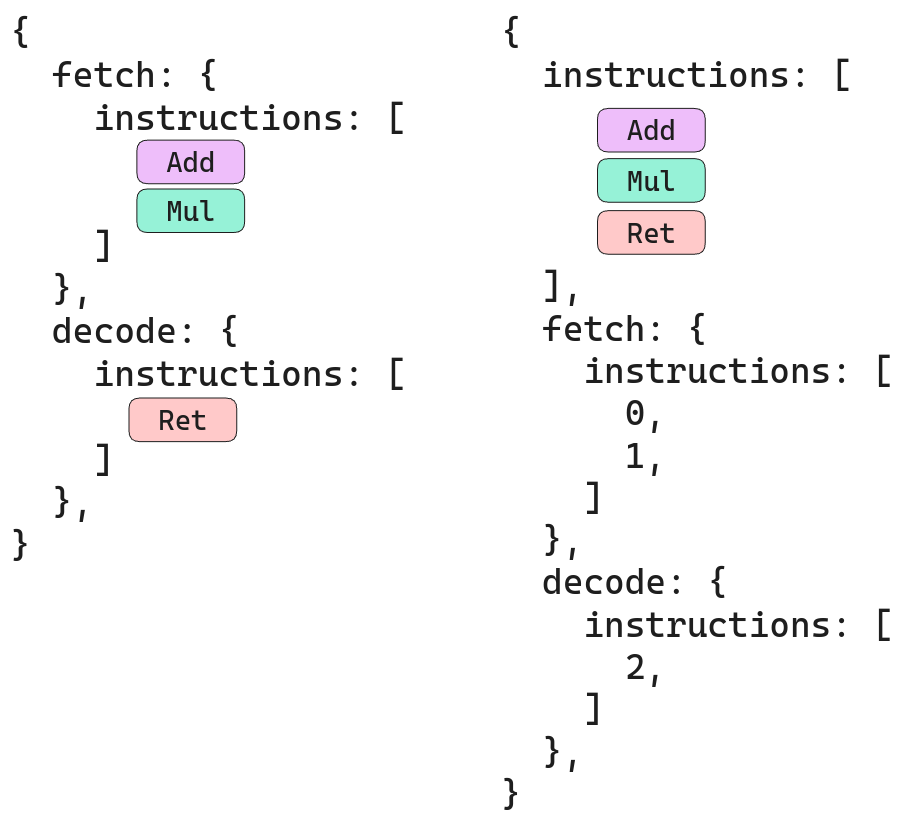
\includegraphics[width=10cm]{obrazky-figures/impl/json_normalization.png}
    \caption{Zjednodušený stav procesoru (vlevo) a jeho normalizovaná verze (vpravo).} 
    \label{json_norm}
\end{figure}

\subsection{HTTP Server}
% Validace, optimalizace (gzip), návrh endpointů
% paralelní
% timeout

Server je implementovaný za pomocí knihovny \emph{Undertow}\footnote{\url{https://undertow.io/}}.
Tato knihovna poskytuje vcelku jednoduché rozhraní pro paralelní obsluhu HTTP požadavků a definici zdrojů (\emph{endpointů}).
Obsluha požadavku je přesunuta do pracovního vlákna, takže obsluha je neblokující.

Všechny endpointy využívají obecnou třídu pro zpracování těla POST požadavku ve formátu JSON, vyvolání daného kódu pro obsluhu a odeslání odpovědi.

HTTP server má konfigurovatelnou adresu (host a port), dobu po které dojde k~vypršení požadavku a přepínač pro použití komprese zip v~odpovědi.

Každý endpoint je definován svou cestou (např. \texttt{/compile}), obsluhovací metodou a datovým typem vstupu a výstupu.
Obsluhovací metoda kontroluje přítomnost povinných parametrů a vykoná aplikační logiku.
Metoda by měla korektně pracovat s~očekávanými chybami a vrátit chybovou hodnotu, která v~daném kontextu dává smysl. 

Neobsloužené výjimky jsou zachyceny serverem a vyřešeny generickou chybovou hláškou, aby nedošlo k~pádu aplikace. 

\subsection{Rozhraní příkazové řádky}
% využití (automatizace)

Rozhraní příkazové řádky nabízenou funkcionalitou odpovídá HTTP serveru.
Místo předávání argumentů v~těle POST požadavku se konfigurace specifikuje soubory.
Všechny parametry rozhraní jsou uvedeny v~příloze \ref{simArgs}.

\subsection{Integrace s~GCC}
% json, params, error reporting

Pro účely překladu programů definovaných v~jazyce C do jazyka RISC-V assembleru HTTP server poskytuje endpoint \texttt{/compile}.
Samotný překlad programu je uskutečněn třídou \texttt{GccCaller}, která poskytuje rozhraní pro volání kompilátoru GCC\footnote{\url{https://gcc.gnu.org/}}.

Proces překladu spočívá ve spuštění nového procesu, který vykoná program GCC s~určitými přepínači (\emph{flags}) a uživatelem zadaným kódem.
Standardní vstup, standardní výstup a standardní chybový výstup procesu jsou přesměrovány do paměti objektu \texttt{GccCaller}.
Návratová hodnota procesu vypovídá o~úspěchu překladu.

Cesta programu GCC je konfigurovatelná při spuštění serveru.
Dále je konfigurovatelná úroveň optimalizace programu.
Povoleny jsou přepínače \texttt{-O0}, \texttt{-O2}, \texttt{-O3} a \texttt{-Os}.
Výčet všech použitých přepínačů se nachází v~tabulce \ref{gccFlags}.

\begin{table}[]
\begin{tabular}{|l|p{8cm}|}
\hline
Přepínač                        & Význam                                                                \\ \hline\hline
\texttt{-xc}                             & Překlad jazyka C (nelze odvodit z~přípony souboru)                    \\ \hline
\texttt{-g} & Mapování řádků jazyka C do assembleru \\ \hline
\texttt{-march=rv32imfd}                 & Definice architektury a rozšíření M, F, D                             \\ \hline
\texttt{-mabi=ilp32d}                    & Generování funkcí s~ABI předávající argumenty registry                \\ \hline
\texttt{-o /dev/stdout}                  & Výstup na standardní výstup                                           \\ \hline
\texttt{-S}                              & Výstup ve formě assembleru                                            \\ \hline
\texttt{-fcf-protection=none}            & Vypnutí bezpečnostních ochran skokových instrukcí                     \\ \hline
\texttt{-fno-stack-protector}            & Vypnutí ochrany proti přetečení bufferů                               \\ \hline
\texttt{-fno-asynchronous-unwind-tables} & Vypnutí generování dat pro obsluhu výjimek                            \\ \hline
\texttt{-mno-explicit-relocs}            & Vypnutí relokace symbolických adres (operátory \texttt{\%hi()} a \texttt{\%lo()})       \\ \hline
\texttt{-ffunction-sections}             & Vytvoření zvláštní sekce pro každou funkci                            \\ \hline
\texttt{-fdata-sections}                 & Vytvoření zvláštní sekce pro každý datový objekt                      \\ \hline
\texttt{-fno-dwarf2-cfi-asm}             & Snížení šumu v~generovaném kódu                                       \\ \hline
\texttt{-finhibit-size-directive}        & Snížení šumu v~generovaném kódu                                       \\ \hline
\texttt{-mstrict-align}                  & Zabránění generování nezarovnaných paměťových přístupů                \\ \hline
\texttt{-nostdlib}                       & Zákaz využití standardní knihovny jazyka C                            \\ \hline
\texttt{-fdiagnostics-format=json}       & Výstup chyb ve formátu JSON                                           \\ \hline
\texttt{-fPIE}                           & Generování pozičně nezávislého kódu (position-independent code)       \\ \hline
\texttt{-fno-plt}                        & Zákaz generování nepřímých skoků pomocí PLT (Procedure Linkage Table) \\ \hline
\end{tabular}
\caption{Jednotlivé přepínače pro překlad. K~těmto přepínačům je ještě přidán přepínač pro žádanou úroveň optimalizace. Většina přepínačů pomáhá generovat čitelnější kód vhodnější ke zpracování simulátorem.}
\label{gccFlags}
\end{table}

Kompilace každého objektu do zvláštní sekce znemožní optimalizace využívající relativní polohu kódu a dat, což je žádoucí vzhledem k~tomu, že data budou v~simulátoru alokována na jinou než předpokládanou pozici.

Existence \texttt{memcmp} a \texttt{memset} je do GCC vestavěna a nelze zabránit generování jejich volání.
Rovněž se mi nepodařilo zakázat volání jiných vestavěných funkcí jako například \texttt{\_\_builtin\_popcount(n)}.
Endpoint tedy programy s~těmito voláními zpracovává a nehlásí chybu, i když s~takovým programem simulátor není schopen pracovat.

% filter
Výstup v~podobě assembleru obsahuje velké množství informací, které jsou pro simulátor nadbytečné a navíc snižují čitelnost kódu.
Proto výstup překladače prochází filtrem, který odstraní nedůležité direktivy, návěstí a data.
Výstupem je tak podstatně čitelnější kód, obsahující pouze relevantní údaje.
Příklad celé transformace je uveden v~\ref{asmFilter}.

\begin{figure}[ht]
     \centering
     \begin{subfigure}[b]{0.4\textwidth}
         \centering
         \begin{lstlisting}
int f(int x) {
    return 2 * x;
}
\end{lstlisting}
         \caption{Vstupní program v~jazyce C.}
         \label{asmFilterA}
     \end{subfigure}
     \hfill
     \begin{subfigure}[b]{0.6\textwidth}
         \centering
         \begin{lstlisting}
  .file "<stdin>"
  .option pic
  .attribute arch, "rv32i2p1_m2p0_f2p2_d2p2_zicsr2p0"
  .attribute unaligned_access, 0
  .attribute stack_align, 16
  .text
  .section .text.f,"ax",@progbits
  .align 2
  .globl f
  .type f, @function
f:
  slli  a0,a0,1
  ret
  .ident "GCC: (Ubuntu 12.3.0-1ubuntu1~22.04) 12.3.0"
  .section .note.GNU-stack,"",@progbits

\end{lstlisting}
         \caption{Assembler před filtrovacím krokem.}
         \label{asmFilterB}
     \end{subfigure}
          \hfill
     \begin{subfigure}[b]{0.4\textwidth}
         \centering
         \begin{lstlisting}
f:
  slli    a0,a0,1
  ret
\end{lstlisting}
         \caption{Kód po filtrování.}
         \label{asmFilterC}
     \end{subfigure}
        \caption{Kroky zpracování programu jazyka C.}
        \label{asmFilter}
\end{figure}

% filter inner workings
Filtr nejdříve rozdělí text na sekce a smaže ty, které nepopisují kód ani data.
Text je dále rozdělen na jednotlivé řádky a řádek assembleru je spojen s~odpovídajícím řádkem programu v~C\footnote{Tento krok souvisí s~vizualizací vysvětlenou v~kapitole \ref{codeEditorPage}.}. 
Dalším krokem je přečtení instrukcí a sběr používaných návěstí.
Na základě této informace jsou smazány všechny direktivy, na které neodkazuje žádné používané návěstí.

Výsledkem je čistý program s~dodatečnou informací o~vztahu mezi řádky původního programu a přeloženého assembleru.
Mapování je využito v~editoru kódu webové aplikace.

\chapter{Implementace webové aplikace}
\label{implementaceweboveaplikace}
% Next.js

Požadavky na aplikaci ze sekce \ref{webAppDesign} lze splnit mnoha způsoby.
Vzhledem k~rozsahu aplikace budu volit z~rámcových řešení pro webové aplikace.
Faktory při výběru frameworku byly popularita, kvalita dokumentace, osobní zkušenost a dispozice knihoven.

Pro implementaci jsem zvolil JavaScriptový framework Next.js\footnote{\url{https://nextjs.org/}}.
Jedná se o~v~současnosti nejrozšířenější způsob psaní aplikací s~knihovnou React.
Jeho hlavními znaky jsou úzké propojení se serverovou stranou a hybridní přístup k~renderování stránek.

% Typescript
Next.js aplikace je možné psát buď v~jazyce JavaScript nebo TypeScript.
Kvůli rozsahu aplikace jsem zvolil TypeScript s~předpokladem, že typové informace usnadní implementaci.

Příloha \ref{gallery} obsahuje více obrázků webové aplikace.

\section{Logika aplikace}
% redux, persistence, global state

Z~pohledu klientské aplikace interaktivní simulace spočívá v~následujících krocích: 
\begin{enumerate}
    \item kontaktovat simulační server s~požadovanou konfigurací,
    \item získat a uložit odpověď (nový stav procesoru),
    \item zpřístupnit nový stav všem relevantním komponentům,
    \item spustit renderování komponentů (prezentace).
\end{enumerate}
Tento postup se opakuje při každém kroku simulace.
Pro implementaci práce se stavem jsem zvolil knihovnu pro správu globálního stavu \emph{Redux}\footnote{\url{https://redux.js.org/}}.

Redux poskytuje rámcové řešení pro popis stavu, přechodů mezi stavy a selektory.
Redux konceptualizuje globální stav jako objekt, který mezi stavy přechází funkcemi zvanými \emph{reducers}.
Jedná se o~čisté funkce, knihovna se zde inspirovala funkcionálním programováním.

Přístup k~části stavu je zprostředkován \emph{selektory}.
Selektor je funkce, která ze stavu vybírá jeho podmnožinu. 
Díky použití selektorů a přechodů je možné určit datové závislosti mezi komponentami a globálním stavem a znovu renderovat pouze ty komponenty, jejichž data byla změněna.

% persist, migrations
Knihovna mi dovolila velmi jednoduše implementovat perzistenci stavu.
Díky tomu je konfigurace zachována mezi sezeními.
Důležité je při každé změně schématu globálního stavu definovat \emph{migraci}, aby aplikace nepracovala se starým, neočekávaným formátem dat.
Tato technika je běžně používaná v~databázích.

% DX - chrome extension
Další přidanou hodnotou je vývojové rozšíření prohlížeče, které umožňuje prohlížet všechny přechody mezi stavy na časové ose.
Detailní náhled stavu umožňuje zobrazit změny z~posledního přechodu (\emph{diff}), nebo aplikaci do zvoleného stavu přenést.
Tyto funkce jsou umožněny transakční/funkcionální architekturou.
Možnost detailně prohlížet stav aplikace mi několikrát usnadnilo řešení problémů.

Globální stav se organizuje do celků s~názvem \emph{slice}.
Jeden slice se má týkat stavu jedné funkcionality.
V~aplikaci jsou 4 slicy:
\begin{itemize}
    \item \texttt{isaSlice} -- ukládá konfigurace procesoru a aktivní konfiguraci,
    \item \texttt{cpustateSlice} -- ukládá aktuální stav interaktivní simulace,
    \item \texttt{compilerSlice} -- obsahuje stav editoru kódu,
    \item \texttt{simConfigSlice} -- obsahuje aktuální simulovanou konfiguraci a kód.
\end{itemize}

% Problém dvou implementací validace vstupů
Jedním z~problémů na který jsem narazil při implementaci byla dvojí implementace kontrola oborů hodnot parametrů.
Jedna implementace se nacházela v~serverové části a druhá ve webové části kódu.
Udržení implementací v~synchronizovaném stavu probíhalo manuálně, což je práce náchylná k~chybám.

\section{Komunikace se serverem}
% server props, caching

Výsledkem překladu projektu ve frameworku Next.js je serverová aplikace a staticky vygenerované zdroje (HTML, CSS, JS).
Prvním požadavkem na server se stáhne statický základ stránky, poté na straně klienta proběhne inicializace Reactu (hydratace) a UI se stává interaktivním.
Veškeré další požadavky na server včetně navigace probíhají přes webové \texttt{fetch API}.

% robots.txt? sitemap?
% https://nextjs.org/docs/app/api-reference/file-conventions/metadata
Webový server kromě stránek, stylů a skriptů nabízí dva statické zdroje: příklady kódů a strukturovaný popis instrukcí RISC-V.
Oba objekty jsou poskytovány přes HTTP API ve formátu JSON.

% sim proxy
První verze řešení využívala přímé volání simulačního serveru, které muselo být nasazeno na adrese dostupné klientovi.
Finální řešení přístup klienta ke službám simulačního serveru zprostředkovává přes webový server, který pracuje jako \emph{proxy}.
Při nasazení je tedy zapotřebí konfigurovat jedinou adresu, na které klient získá i webové rozhraní i simulační služby.
Celá komunikace je nastíněna na obrázku \ref{diagramApiComms}.

\begin{figure}[ht]
    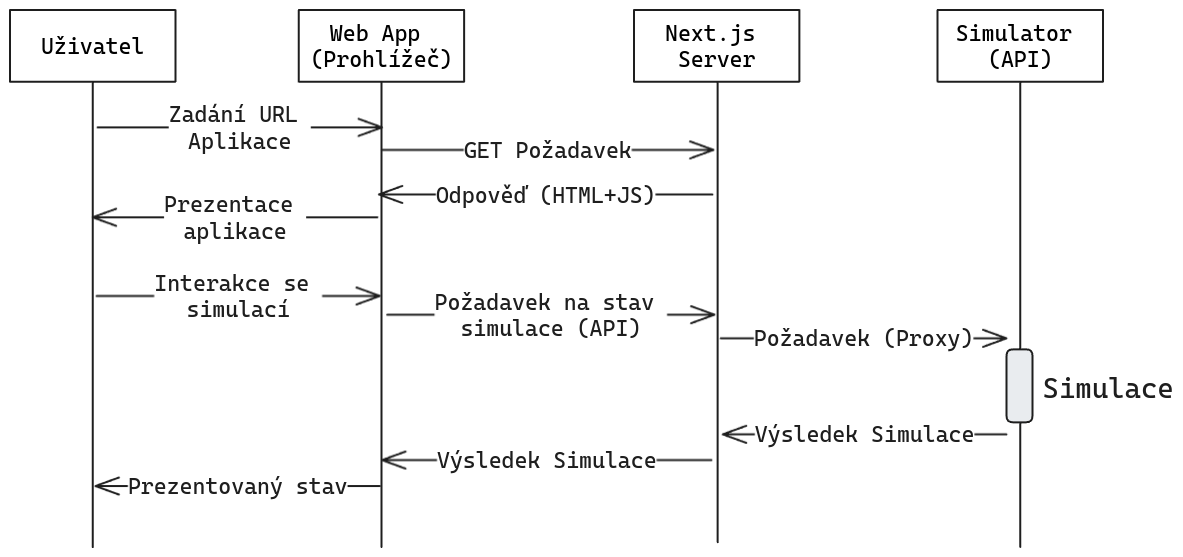
\includegraphics[width=\textwidth]{obrazky-figures/impl/apicomms.png}
    \caption{Sekvenční diagram komunikace prohlížeče a serveru.}
    \label{diagramApiComms}
\end{figure}

Odpověď simulačního serveru je uložena do globálního stavu, čímž spustí renderování nového stavu simulace.
Redux umožňuje narušit funkcionální povahu přechodů mezi stavy a při přechodu provést HTTP dotaz. 

% caching, prefetching
Framework Next.js ve výchozím nastavení poskytuje mnoho optimalizací.
Mezi nejvýznamější patří caching a prefetching zdrojů.
Výsledkem prefetchingu odkazů zobrazených na stránce ve výsledku znamená okamžitou navigaci mezi stránkami. 

\section{Stránky}
% nebo "pohledy/views"
% settings, layouts, side menu

Aplikace se skládá z~osmi hlavních pohledů.
V~následujících podsekcích rozvedu některé z~jednotlivých stránek, jejich účel a způsob implementace.

% ostatní stránky, moc krátké na podsekci

Stránka nastavení poskytuje pouze tři funkce -- smazaní lokálního úložiště, export dat a výběr mezi světlou a tmavou barevnou paletou.

\subsection{Simulační okno}
\label{simWindow}

% todo welcome popup

Simulační okno je jádrem celé aplikace.
Je zároveň nejsložitější částí aplikace.
Okno obsahuje schéma procesoru a dva samostatné prvky: horní ovládací menu a pravou lištu.

% posuvné okno
% bloky, trasy, zvětšování
Prostřední část okna je věnována schématu procesoru.
Vedle sebe zde leží rozmístěny jednotlivé obdélníkové bloky, které odpovídají blokům v~simulátoru.
Mezi bloky vedou spoje, které naznačují jejich souvislost.

Všechny bloky sdílejí ovládací prvky.
Blok jednotky fetch je uveden na obrázku \ref{simblock_figure}.
V~horní části vedle názvu bloku (1) se nachází tlačítko (4) vyvolávající vyskakovací okno s~detailem bloku.
Pod ním je několik nejdůležitějších informací o~aktuálním stavu (2).
Potažením pravého dolního rohu (5) se dá změnit velikost bloku.
Rozmístění bloků je k~této změně responzivní.
Zbytek plochy je specifický pro každý druh bloku.
Nejčastěji obsahuje seznam instrukcí (3), které se v~bloku momentálně nacházejí.

\begin{figure}[hbtp]
    \begin{center}
        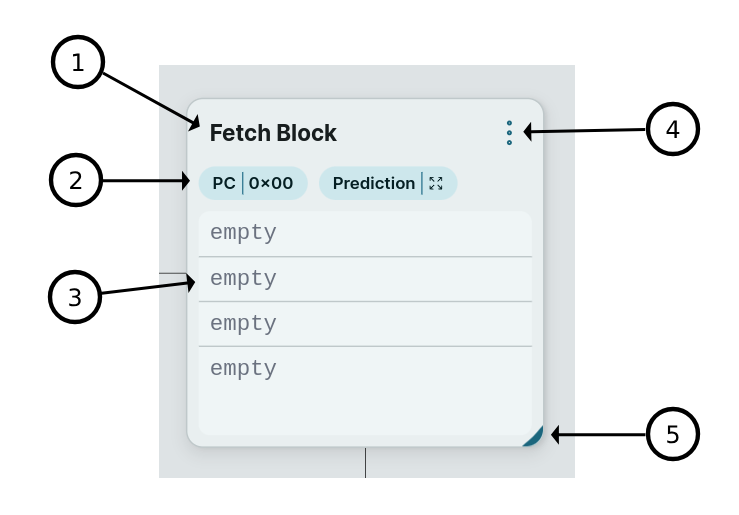
\includegraphics[width=11cm]{obrazky-figures/impl/simblock.png}
    \end{center}
    \caption{Reprezentace bloku Fetch.}
    \label{simblock_figure}
\end{figure}

Celý pohled na procesor lze posouvat a přibližovat.
Technicky je této možnosti docíleno sledováním pohybu myši nad oknem a přepočítáváním odsazení všech bloků od počátku souřadného systému.

% ovládání simulace, zkratky, automatika
Simulaci je možno ovládat jak myší, tak i klávesnicí.
Pro ovládání myší je v~horní části obrazovky menu s~tlačítky umožňující krok v~simulaci dopředu nebo zpět, skok na začátek nebo konec simulace.
Stejné možnosti jsou k~dispozici klávesovými zkratkami.
Druhé menu v~horní části obrazovky nabízí automatické krokování simulace.
Prodleva mezi kroky je nastavitelná v~textovém poli.

% detaily bloků a instrukcí
Schématický pohled na stav simulace poskytuje celkový přehled, nemůže ale zobrazit všechny detaily, které jsou k~dispozici.
K~tomu slouží vyskakovací náhledy.
Kliknutím na blok nebo instrukci se objeví okno, které v~tabulkové formě poskytuje dostupné informace.
Pro instrukce se jedná o~časové známky důležitých aktivit (fetch, execute), hodnoty paramtetrů a příznaky (například zda je instrukce spekulativní, či zda jsou všechny parametry připraveny k~vykonání).
Detaily bloků jsou specifické pro každý blok.
Například detail bloku hlavní paměti (na obrázku \ref{mainmemory_popup_figure}) ukazuje všechny ukazatele v~programu, jejich adresy a větší znázornění celé paměti.

\begin{figure}[hbtp]
    \begin{center}
        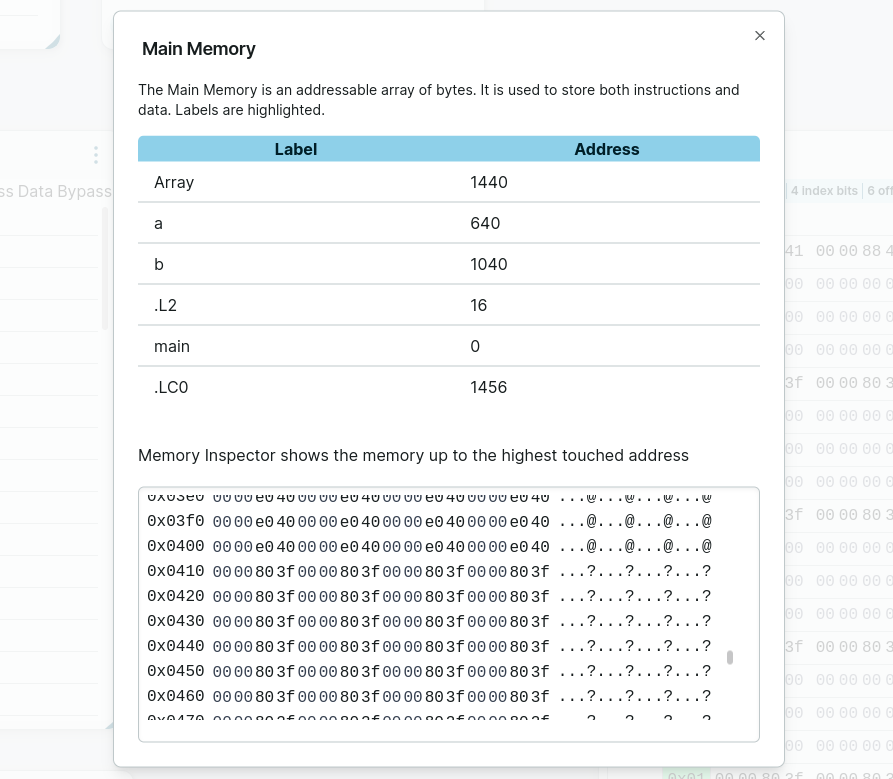
\includegraphics[width=12cm]{obrazky-figures/impl/mainmemory_popup.png}
    \end{center}
    \caption{Detail bloku hlavní paměti.}
    \label{mainmemory_popup_figure}
\end{figure}

% přejetí nad instrukcí nebo registrem
% hover bubliny
Po najetí na instrukci nebo registr se zvýrazní všechny jejich výskyty v~ostatních blocích.
Tato funkce je velmi užitečná pro zorientování ve stavu simulace. 
Implementace je rozvedena v~sekci \ref{optimRender}, kde je popsán i proces její optimalizace.
Po najetí myší na parametr instrukce se také objeví bublina s~jeho hodnotou.
U~registru se navíc objeví informace o~jeho přejmenování. 

% lišta - statistiky, log
Lišta na pravé straně zobrazuje vybrané statistiky a log.
Lišta má dva stavy: výchozí a expandovaný.
V~expandovaném stavu vzniká místo pro více statistik a textu zpráv z~logu.
Ke zobrazení jsem vybral statistiky, které považuji za nejrelevantnější při simulování: počet taktů, počet vydaných instrukcí, IPC a úspěšnost predikce skoků.
Kompletní statistiky jsou zobrazeny na zvláštní stránce (viz sekce \ref{statsPage}).
Každá zpráva v~logu má svou časovou známku (takt, kdy zpráva vznikla).
Kliknutím na číslo zprávy se simulace do tohoto taktu přenese.

% obrázek s očíslovanými šipkami na prvky

\subsection{Editor kódu}
\label{codeEditorPage}

Editor (na obrázku \ref{codeeditor_figure}) nabízí lištu s~akcemi a dvě textová pole.
V~levém sloupci lze ovládat kompilaci.
Prostřední okno slouží k~psaní kódu v~jazyce C, pravé okno zobrazí výsledek překladu.

Textová pole jsou implementována za pomocí knihovny CodeMirror\footnote{\url{https://codemirror.net/5/}}.
Tato knihovna poskytuje dobré uživatelské rozhraní pro editaci kódu, například běžné zkratky, zvýraznění syntaxe, zobrazení varování, očíslování řádků a další.
Důležitá byla i možnost vytvořit vlastní rozšíření.

\begin{figure}[hbtp]
    \begin{center}
        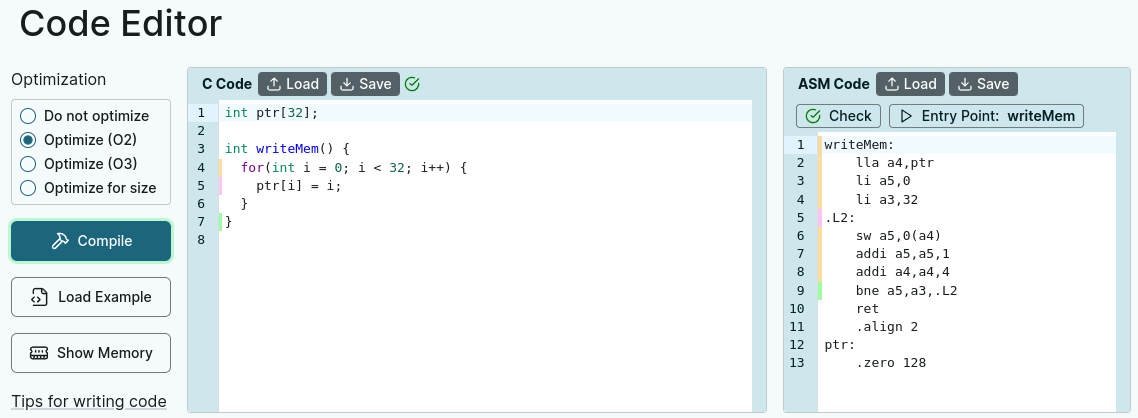
\includegraphics[width=15cm]{obrazky-figures/impl/codeeditor.png}
    \end{center}
    \caption{Editor kódu s kompilátorem.}
    \label{codeeditor_figure}
\end{figure}

Souvislost částí kódu je naznačena barevným páskem na levé straně textového pole.
Najetím myší na skupinu řádků se vztah vyznačí výrazněji.
Při najetí myší na instrukci (obrázek \ref{codeeditorhover_figure}) se také objeví vyskakovací okno s~informací o~argumentech instrukce.

\begin{figure}[hbtp]
    \begin{center}
        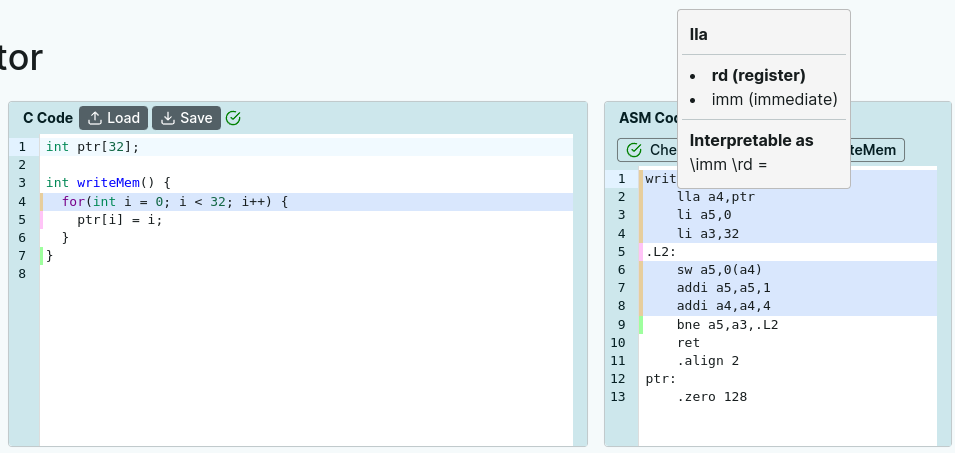
\includegraphics[width=15cm]{obrazky-figures/impl/codehover.png}
    \end{center}
    \caption{Vzhled editoru při najetí myší na instrukci.}
    \label{codeeditorhover_figure}
\end{figure}

O~vyznačení chyb v~textovém poli se stará knihovna CodeMirror, chyby je ale nutné z~výstupu simulátoru převést do správného formátu.
Chybná část kódu je podtržena, po najetí na oblast myší je zobrazena chybová zpráva (viz obrázek \ref{codeerrors}).
Zpráva o~chybách nebo úspěchu překladu se také objevuje v~rohu obrazovky.

\begin{figure}
     \centering
     \begin{subfigure}[b]{0.56\textwidth}
         \centering
         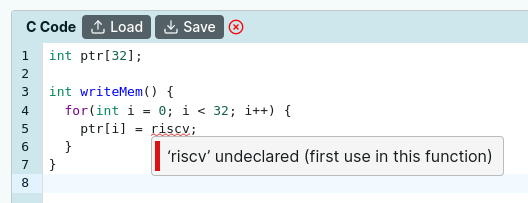
\includegraphics[width=\textwidth]{obrazky-figures/impl/c_error.png}
         \caption{Chyba v~programu jazyka C. Hlášení jsou předávána z~kompilátoru GCC.}
         \label{fig:codeerrors1}
     \end{subfigure}
     \hfill
     \begin{subfigure}[b]{0.42\textwidth}
         \centering
         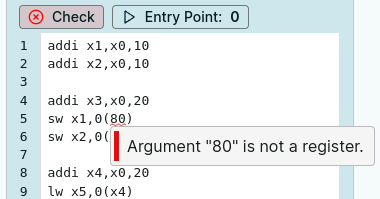
\includegraphics[width=\textwidth]{obrazky-figures/impl/asm_error.png}
         \caption{Chyba v~Assembleru RISC-V. Hlášení pochází z~vlastního kompilátoru assembleru (viz sekce \ref{parsingAsmCode}).}
         \label{fig:codeerrors2}
     \end{subfigure}
        \caption{Zobrazení chyb v~editoru.}
        \label{codeerrors}
\end{figure}


V~neposlední řadě je zde možné zvolit vstupní bod programu.
Vstupním bodem může být první instrukce, nebo libovolné návěstí.

\subsection{Konfigurace paměti a procesoru}
% formuláře

Konfigurace paměti (simulačních dat) a procesoru jsou formulářové stránky.
Obsahují velké množství vstupních textových polí s~názvem, vysvětlivkami a validací.
Formuláře kopírují strukturu konfigurace simulátoru.

Logika formulářů je implementována pomocí knihovny \emph{React Hook Form}.
Schéma formuláře je definováno objekty validační knihovny \emph{Zod}.

Vstupní textové pole a přepínač (\emph{radio input}) jsou znovupoužitelné komponenty.

Konfigurace procesoru je rozdělena do záložek, které všechny možnosti organizují do kategorií.
V~horní části obrazovky je možné přepínat mezi uloženými konfiguracemi, nebo založit konfiguraci novou.
Zvláštním prvkem formuláře je \uv{podformulář} pro definice funkčních jednotek.

Konfigurace paměti umožňuje přidávat, upravovat a mazat datové objekty.
Datový objekt má jméno, zarovnání, datový typ a samotná data.
Data je možné definovat několika způsoby:
\begin{enumerate}
    \item explicitním výčtem prvků,
    \item opakováním konstanty (po vzoru \texttt{memset}),
    \item rozsahem náhodných prvků (např. 32 čísel v~rozsahu 0-15).
\end{enumerate}
Formulář nemá plnou vyjadřovací schopnost -- jsou konfigurace paměti, které lze definovat pouze ručně psanou definicí ve formátu JSON.
Takové definice ale lze do webové aplikace importovat a pracovat s~nimi.

\subsection{Statistiky}
\label{statsPage}

Jak bylo zmíněno v~sekci o~hlavním simulačním okně (\ref{simWindow}), nejdůležitější statistiky jsou zobrazeny v~boční liště při simulaci.
Detailnější pohled na sbírané statistiky je k~dispozici ve speciálním okně.

Stránka je organizovaná do karet podle kategorií statistik.
Tři karty jsou ukázány na obrázku \ref{stats_screenshot}.
Modul na pravé straně ukazuje statistiky ke konkrétní instrukci v~podobě \emph{teplotní mapy}.
Lze v~něm přepnout mezi pohledem na úspěšnost nalezení dat v~cache a podílem vydaných instrukcí v~průběhu programu.

\begin{figure}[hbtp]
    \begin{center}
        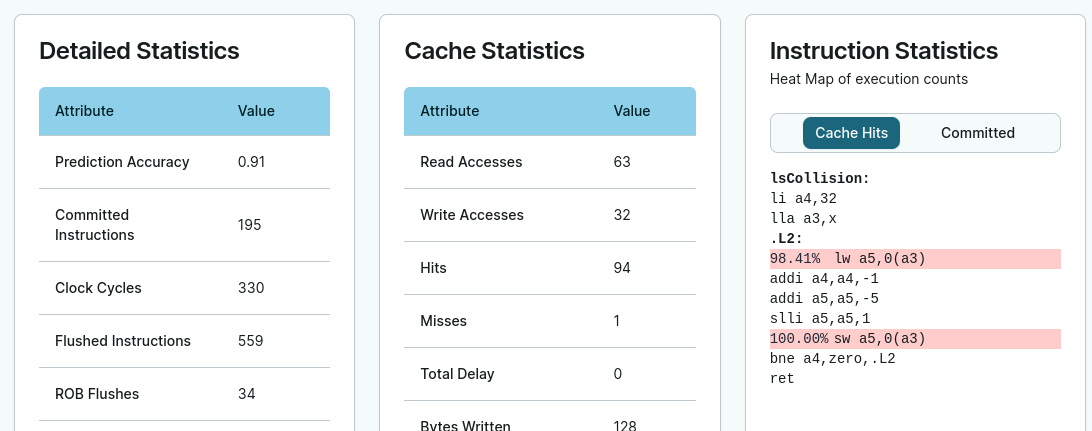
\includegraphics[width=15cm]{obrazky-figures/impl/stats.png}
    \end{center}
    \caption{Výřez obrazovky statistik poskytovaných na vyhrazené stránce.}
    \label{stats_screenshot}
\end{figure}

\subsection{Edukativní stránky}

Součástí aplikace je krátký informativní úvod do architektury RISC-V.
Tento text vysvětluje základní informace o~registrech a konvenci volání, což může být užitečné pro někoho, kdo má zkušenosti s~assemblerem, ale ne konkrétně s~RISC-V.
Pro hlubší porozumění jsou poskytnuty odkazy na detailnější materiály.

Jiná edukativní stránka se věnuje přehledu architektury procesoru.
Každému důležitému komponentu je věnována krátká sekce.

Poslední stránkou je nápověda.
Ta uvádí zkratky, kterými je možné simulaci ovládat.
Obsahuje také tipy pro psaní kódu pro simulátor, včetně jeho specifik a odchylek.

\section{Design a použitelnost}
% barevné schéma, layout a hierarchie, nápovědy
% shad/cn, radix, tailwindcss, lucide icons
% vizualizace (prediktorů)

% component libraries
Mnoho komponentů (například formuláře, nebo karty objevující se po přejetí myší a vyskakovací okna) je implementovaných pomocí knihoven předpřipravených komponentů.
Tyto komponenty zajišťují dobrou úroveň dostupnosti a správné chování napříč zařízeními.
Zároveň umožňují detailní úpravu podle požadavků programátora.

Komponenty jsou stylovány kombinací CSS a stylovací knihovny \emph{TailwindCSS}\footnote{\url{https://tailwindcss.com/}}, která poskytuje obecné stylovací třídy.
Na stránkách jsou využity sémantické značky HTML (například \texttt{<section>}, \texttt{<nav>}, které přesněji vyjadřují význam částí stránky.

% barevná paleta, dark mode
Navrhnout vhodnou a funkční barevnou paletu je těžký designový úkol, který byl přenechán nástroji \emph{Material Theme Builder}\footnote{\url{https://m3.material.io/theme-builder}}.
Algoritmus od společnosti Google, který se používá v~operačním systému Android, generuje vizuálně zajímavou paletu splňující požadavky na kontrast.
Paleta má také variantu pro tmavý režim rozhraní.
Obrázek \ref{lightanddarkmode} ukazuje porovnání světlé a tmavé palety rozhraní.
% TODO https://material.io/blog/science-of-color-design

% Tab navigation
Zvláštní důraz byl kladen na možnost ovládat celou aplikaci klávesnicí.
Motivací bylo dát všem uživatelům tuto možnost, neméně důležité ale bylo udělat maximum pro dobrou dostupnost aplikace.
Rozhraní simulace obsahuje velké množství interaktivních prvků (dlouhé tabulky instrukcí), což může učinit navigaci na konkrétní prvek zdlouhavé.
Tento nedostatek není zcela vyřešen, prázdná pole jsou ale při navigaci ignorována.

Zobrazení aplikace je optimalizováno pro všechny velikosti obrazovky.
Obrázek \ref{mobile_layout} jako příklad ukazuje rozložení stránky kompilátoru na mobilním zařízení (obrázek \ref{codeeditorhover_figure} ukazuje stejnou část rozhraní na široké obrazovce stolního počítače).
Prvky mají užší okraje a komponenty jsou uspořádány vertikálně.
Aplikaci je možné na mobilním zařízení úspěšně používat, omezení malé dotykové obrazovky ale snižuje pohodlí.

\begin{figure}[hbtp]
\centering
    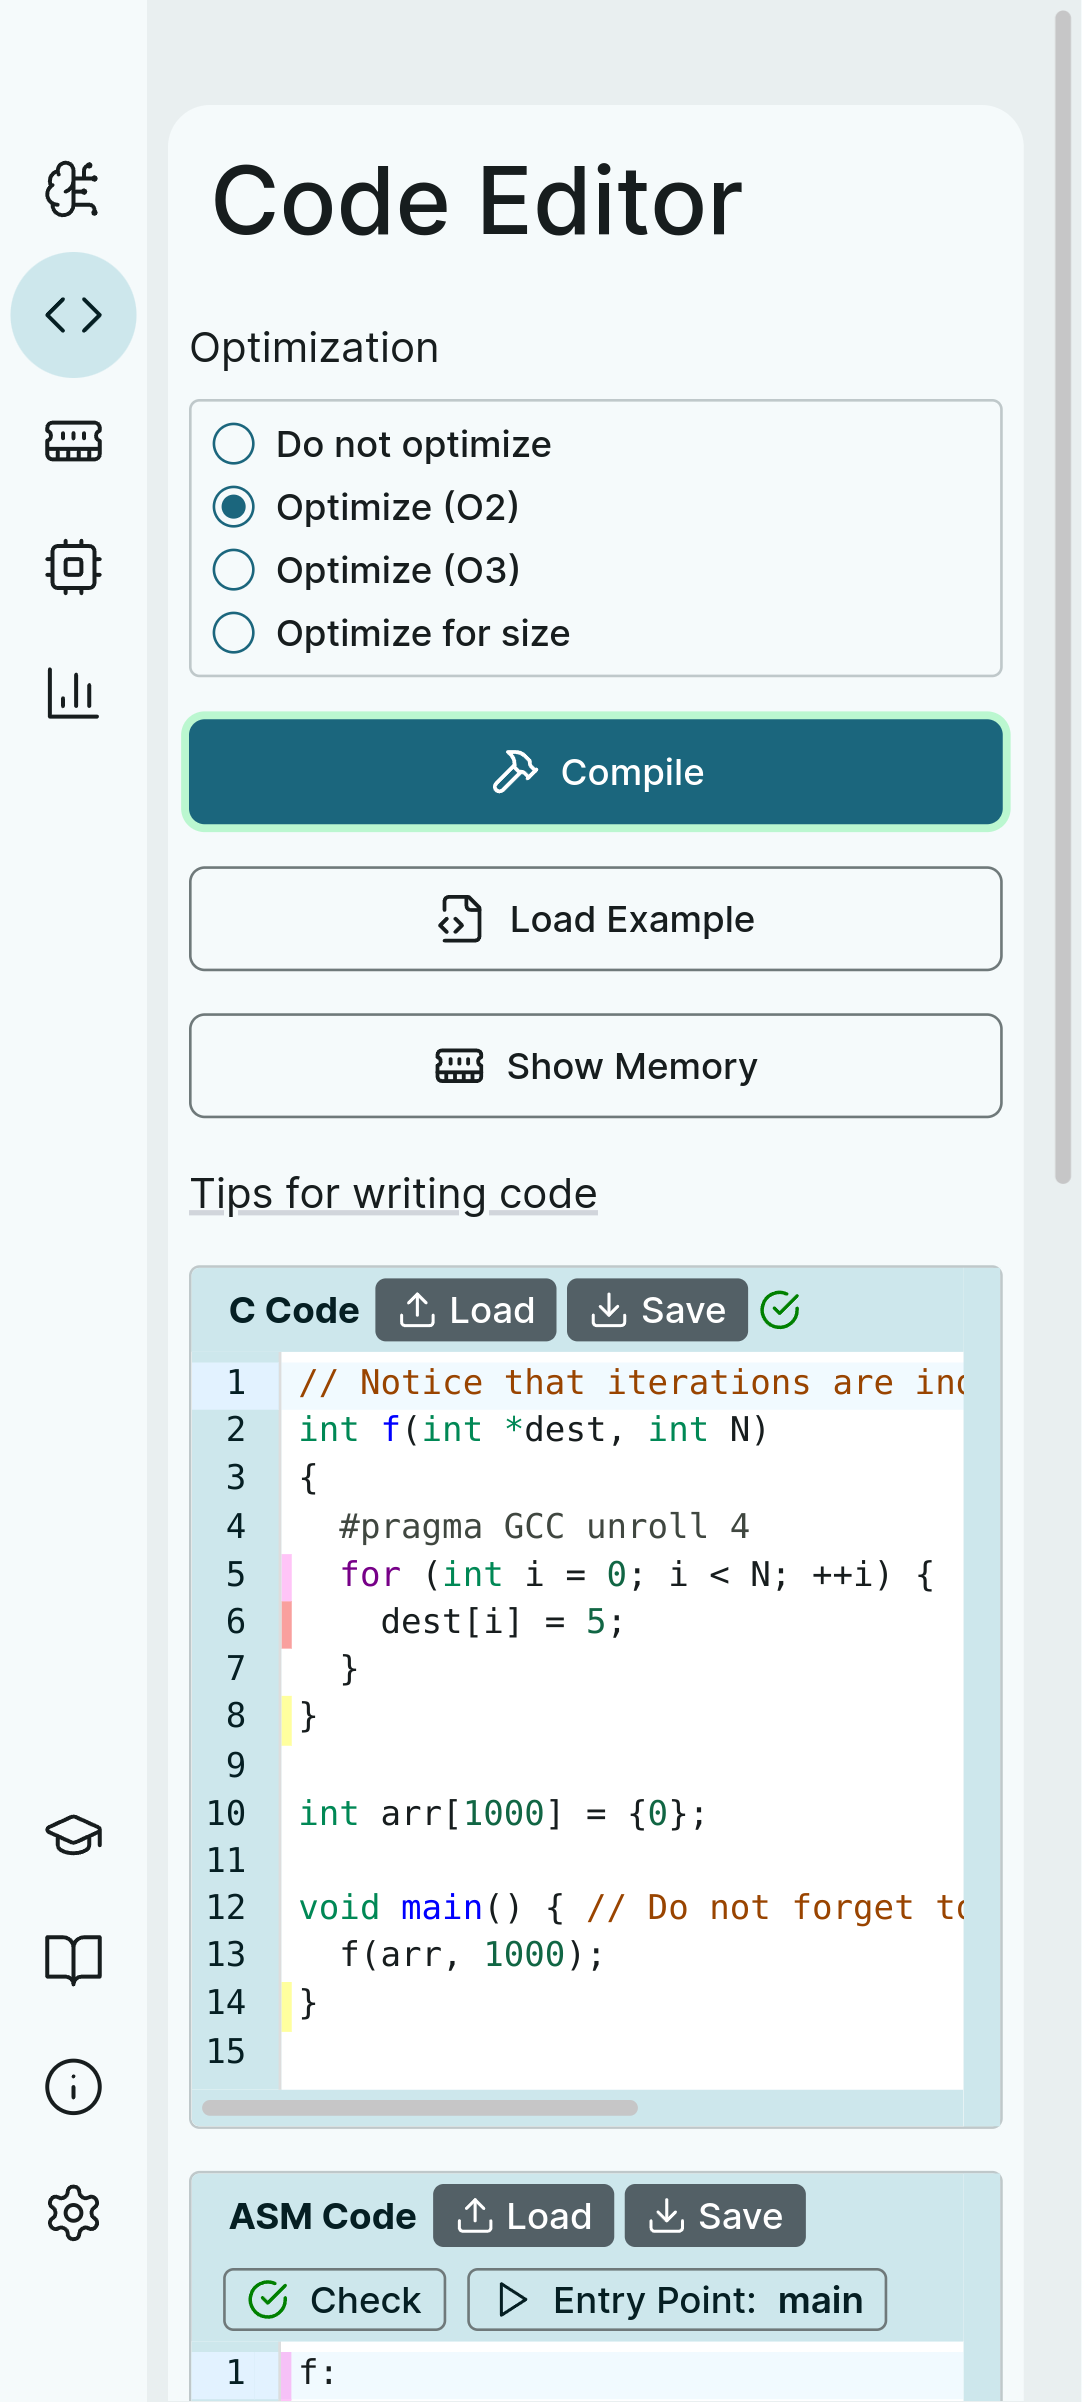
\includegraphics[width=9cm]{obrazky-figures/impl/mobile_layout_compiler.png}
    \caption{Pohled kompilátoru v~rozložení pro mobilní telefony.} 
    \label{mobile_layout}
\end{figure}



\begin{figure}
     \centering
     \begin{subfigure}[b]{0.49\textwidth}
         \centering
         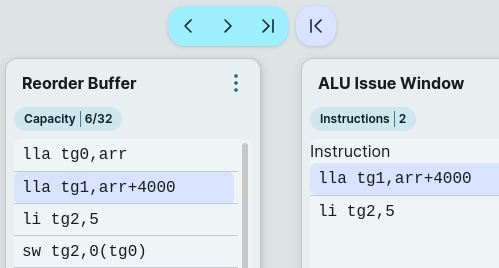
\includegraphics[width=\textwidth]{obrazky-figures/impl/lightmode.png}
         \caption{Simulátor ve světlém režimu rozhraní.}
         \label{fig:lightmode}
     \end{subfigure}
     \hfill
     \begin{subfigure}[b]{0.49\textwidth}
         \centering
         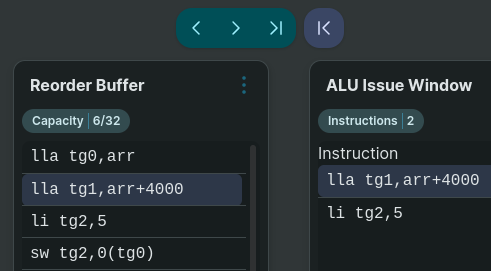
\includegraphics[width=\textwidth]{obrazky-figures/impl/darkmode.png}
         \caption{Simulátor v~tmavém režimu rozhraní.}
         \label{fig:darkmode}
     \end{subfigure}
        \caption{Světlá a tmavá varianta palety barev.}
        \label{lightanddarkmode}
\end{figure}

\subsection{Komponenty rozhraní, React}
% nextjs

Rozhraní je členěno do hierarchie komponentů.
Většina komponentů je definovaných ve zvláštním souboru, ale některé příliš specifické komponenty se nachází v~souboru společně s~místem použití.

Při návrhu uživatelského rozhraní pomocí React komponentů byly dodržovány zásady jediné odpovědnosti (SRP), což pomohlo udržet každou komponentu co nejvíce oddělenou a specializovanou na svou úlohu.
Každá komponenta byla navržena s~definovaným účelem, rozhraním a funkcionalitou, což usnadňuje správu kódu a jeho budoucí rozšíření.
Komponenty jsou ve struktuře projektu organizovány podle stránek nebo účelu, ke kterému náleží.

Dalším důležitým principem byla znovupoužitelnost.
Některé komponenty jsou využívány v~různých částech aplikace a v~různých kontextech.
Příkladem je komponent pro zobrazení programu, který je využitý jak v~simulačním tak statistickém okně.

\subsection{Optimalizace renderování}
\label{optimRender}
% memo, dělení do komponentů
% profilování

% Přesun do css
% todo české uvozovky
Důležitou součástí rozhraní simulace je interaktivní zvýraznění všech výskytů instrukce nebo registru napříč bloky.
První řešení informaci o~novém \uv{aktivním} prvku zapisovalo do globálního stavu.
Styl zvýraznění byl vypočítáván JavaScriptem, takže změna stavu spustila renderování \emph{celého} náhledu.
Tento přístup nebyl optimální a negativně se projevoval na responzivitě rozhraní.
Přejetím kurzoru napříč oknem se mohly vykonat i desítky událostí způsobujících renderování.

Řešením bylo přesunutí datové závislosti z~Reactu do CSS.
Jádro řešení zůstává stejné -- JavaScript stále naslouchá události najetí myši na instrukci a změny se stále zapisují do globálního stavu.
Důležitým rozdílem je, že změna stavu vyvolává změnu v~dynamicky generovaném kaskádovém stylu místo změny v~závislostech Reactu. 
Vyhodnocení CSS pravidel probíhá v~kódu prohlížeče, který je mnohem výkonnější.
Stylování probíhá pravidlem, které vybírá elementy na základě hodnoty jeho atributu (ID).
Po implementaci této optimalizace probíhá zvýrazňování okamžitě.

% virtual lists
% in extreme, 11700 DOM elements -> 6500 elements
Druhou významnou optimalizací bylo využití virtuálních rolovacích seznamů v~blocích, které zobrazují velké množství prvků.
Virtuální seznam využívá předpokladu, že většina prvků seznamu není zobrazených ve stejný okamžik.
Renderovány jsou jen ty prvky, které mají být v~daný okamžik viditelné.
Jestli má prvek být viditelný je vypočteno na základě velikosti prvků v~seznamu a velikosti rolovacího okna.

Implementace optimalizace se projevila významným snížením doby renderování, obzvlášť v~náhledu do hlavní paměti procesoru, který má velké množství elementů.
Při pokusu jsem naměřil pokles v~počtu HTML elementů na stránce z~11700 na ~6500.

\chapter{Testování, dokumentace a nasazení}
\label{testingchapter}
% formát kódu a komentářů (handbook sc fit)
% vývojové praktiky

V~této kapitole budou popsány okolní činnosti související s~vývojem aplikace.
Zejména se zaměří na testování simulátoru a webové aplikace.

%docs
% Java: 173 souborů, 10735 komentářů, 19577 kódu => cca 5545 bez hlaviček
% TS:   130 souborů, 4541 komentářů, 12073 kódu => cca 640 bez hlaviček
Celý projekt obsahuje asi 33\,000 řádků kódu (bez komentářů a prázdných řádků).
Velikost projektu je uvedena pro kontext množství komentářů: asi 6\,000 řádků (15\,000 včetně hlaviček souborů).
Při refaktorizaci simulátoru byl razantně zvýšen počet komentářů, jak v~hlavičkách funkcí a tříd, tak uvnitř kódu.
% todo spočítat počty komentářů

Během vývoje byl využit systém pro správu verzí \texttt{git}.
Kód byl před každým sloučením do hlavní větve prověřen vedoucím práce. 

V~projektu byl použit styl kódu z~příručky \emph{Handbook SC FIT} (příručky pro skupinu SC@FIT). 
Použití jasně definovaných pravidel pro úpravu kódu zajišťuje konzistenci a přehlednost kódu, která usnadňuje orientaci a úpravy pro současné i budoucí členy týmu.

\section{Testování simulátoru}
% Testování příkladů
% todo coverage

%todo pomohly mi logy při uživatelském testování

Během implementace simulátoru (sekce \ref{implSimulace}) byly intenzivně využívány jak existující testy, tak nově vytvořené testy, které byly postupně doplňovány.
Testy zvyšovaly důvěru ve správnost úprav i nových funkcí simulátoru.
Projekt v~současném stavu obsahuje více než 400 testů.
Pokrytí řádků kódu testy v~simulátoru je 83\%.
Pokrytí v~blocích simulátoru je 94\%.

Jednotkové testy (unit tests) testují izolované moduly.
Izolované testování jednotlivých tříd a systémů simulátoru bylo stěžejním pro úspěšnou implementaci.
Důkladněji testované byly moduly Cache, prediktory a překlad kódu.
Kód byl navrhován tak, aby byl deterministický a problémy reprodukovatelné, což zjednodušuje testování.


% dynamic dispatch works
Systém byl jako celek testován z~mnoha aspektů.
Každá instrukce má svůj test kontrolující její správné chování.
Tento typ testů typicky kontroluje stav na konci simulace.
Testovací skript navíc kontroluje, že všechny přiložené ukázky kódu proběhnou na simulátoru bez chyby.

Jedna sada testů simulátoru je velmi detailní a stav kontroluje po každém taktu.
Detailní testy jsou zákonitě více spjaté s~implementací a vyžadují větší množství údržby.

Je také testována funkčnost několika složitějších programů jako například třídění pole algoritmem \emph{quicksort}, práce s~lineárním seznamem a polymorfismus (\emph{dynamic dispatch}).

\subsection{Výkonnostní testování}
% při provozu serveru asi 70% času zabírá serializace
% 1/3 běhu simulace je parsování kódu (před optimalizací). Hodně trvá inicializace
% z requestu na tick 1 je 10% resolve(), 1,5% samotná simulace
% profiler visualvm

Pro testování výkonu byl simulátor profilován v~režimu server.
V~rámci testování také vznikl jednoduchý benchmark implementovaný pomocí Java Microbenchmark Harness (JMH).

Nejdůležitějším závěrem z~testování výkonu je následující:
v~režimu serveru asi 60\% doby obsloužení požadavku zabírá práce s~formátem JSON.
Tento formát je ze své povahy nepříznivý pro výkon.
Důsledkem dominance komunikační marže je, že výkonnostní zisky z~optimalizace simulace se přestávají vyplácet.
Změna komunikačního protokolu je směr, který je zajímavý v~další práci prozkoumat.

% rampup 4s

% local
% Notebook Intel i5 8300h, 16GB DDR4 RAM
% bez dockeru
%
% 30 uživatelů, 1s mezi requesty, 40 kroků simulace: medián latence 70.66ms, 90percentil 118.00ms, throughput 25.96 transakcí/sec
%
% 100 uživatelů, 1s mezi requesty, 40 kroků simulace: medián latence 680ms, 90percentil 1248.90ms, throughput 53.61 transakcí/sec

% local
% Notebook Intel i5 8300h, 16GB DDR4 RAM
% docker
%
% 30 uživatelů, 1s mezi requesty, 40 kroků simulace: medián latence 77.00ms, 90percentil 283.00ms, throughput 24.49 transakcí/sec
%
% 100 uživatelů, 1s mezi requesty, 40 kroků simulace: medián latence 1135.00, 90percentil 2031.90, throughput 42.07 transakcí/sec

Proběhlo také zátěžové testování nástrojem Apache JMeter™\footnote{\url{https://jmeter.apache.org/}}.
Charakteristika testu je následující:
\begin{itemize}
    \item dvě velikosti testu: 30 a 100 uživatelů,
    \item dva běhové režimy: přímý a prostřednictvím Dockeru,
    \item každý uživatel interaktivně simuluje 40 kroků simulace jednoho ze dvou programů,
    \item náběh 4\,s, 1\,s pauzy mezi každým požadavkem uživatele (think time),
    \item použití gzip,
\end{itemize}
Použitím komprese gzip se zvýšila propustnost na lokálním serveru o~40\%.
Tabulka \ref{apachePerfDataTable} uvádí naměřená data.
Veškeré měření proběhlo lokálně na notebooku s procesorem \texttt{Intel i5 8300h} a 16\,GB DDR4 RAM.
Závěrem je, že server dobře zvládá menší množství současných uživatelů, bez ohledu na běhový režim, i když Docker má znatelný dopad na výkon aplikace.
Větší množství uživatelů výrazně negativně ovlivňuje latenci takovým způsobem, že se výrazně zhorší komfort užívání aplikace.
Během testu nedošlo ani k~pádu aplikace ani k~selhání dotazu.
V~reálném provozu bude latence pravděpodobně vyšší v~důsledku delší cesty paketů internetem.
Větší množství uživatelů je možné řešit provozem na silnějším hardwaru, nebo rozdělením zátěže mezi několik serverů.

% TODO: přejmenovat "přímý" režim?
\begin{table}[]
\centering
\begin{tabular}{|l|r|rr|r|}
\hline
\multirow{2}{*}{Režim}  & \multicolumn{1}{l|}{\multirow{2}{*}{Počet uživatelů}} & \multicolumn{2}{l|}{Latence (ms)}                                & \multicolumn{1}{l|}{\multirow{2}{*}{Propustnost (transakce/s)}} \\ \cline{3-4}
                        & \multicolumn{1}{l|}{}                                 & \multicolumn{1}{l|}{Medián} & \multicolumn{1}{l|}{90. percentil} & \multicolumn{1}{l|}{}                                   \\ \hline
\multirow{2}{*}{Přímý}  & 30                                                    & \multicolumn{1}{r|}{70,66}  & 118                                & 25,96                                                   \\ \cline{2-5} 
                        & 100                                                   & \multicolumn{1}{r|}{680}    & 1248,9                             & 53,61                                                   \\ \hline
\multirow{2}{*}{Docker} & 30                                                    & \multicolumn{1}{r|}{77}     & 283                                & 24,49                                                   \\ \cline{2-5} 
                        & 100                                                   & \multicolumn{1}{r|}{1135}   & 2031,9                             & 42,07                                                   \\ \hline
\end{tabular}
\caption{Naměřené hodnoty latence pro 4 uvedené případy.}
\label{apachePerfDataTable}
\end{table}

Na obrázku \ref{responseTimes} jsou uvedeny dva grafy latence odpovědí serveru.
U~obou testů lze pozorovat, že latence se drží v~určitých mezích a nerostou neomezeně.
Zvýšená zátěž nikdy během testování nezpůsobila odmítnutí požadavku.

\begin{figure}
  \centering
  \begin{tabular}{@{}c@{}}
    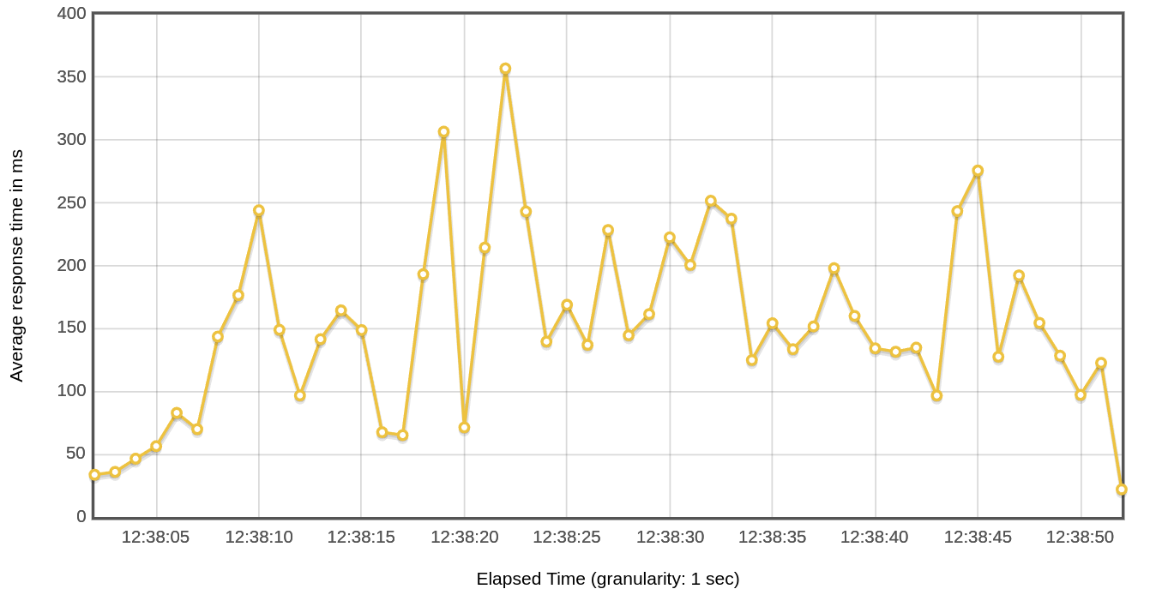
\includegraphics[width=\linewidth]{obrazky-figures/perf/local_metal_30_responseTimesOverTime.png} \\[\abovecaptionskip]
    \small (a) Průběh latence odpovědi od serveru v~čase pro 30 současných uživatelů.
  \end{tabular}

  \vspace{\floatsep}

  \begin{tabular}{@{}c@{}}
    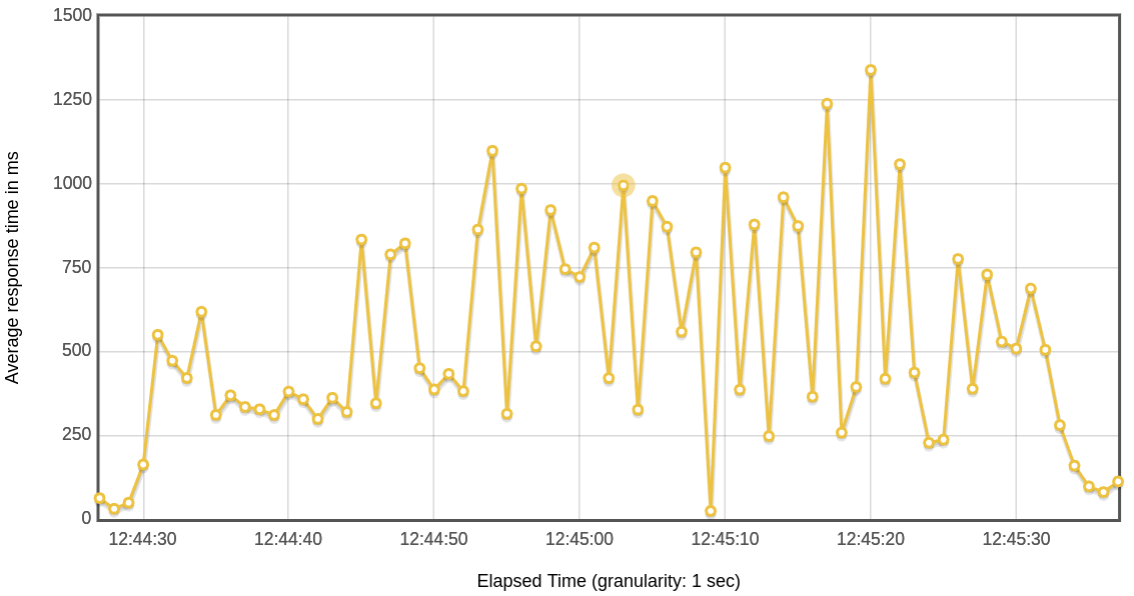
\includegraphics[width=\linewidth]{obrazky-figures/perf/local_metal_100_responseTimesOverTime.png} \\[\abovecaptionskip]
    \small (b) Průběh latence odpovědi od serveru v~čase pro 100 současných uživatelů.
  \end{tabular}

  \caption{Grafy latence serveru při interaktivní simulaci.}
  \label{responseTimes}
\end{figure}

\section{Testování webu}

Webová část projektu byla testována především manuálně.
Uživatelská rozhraní jsou proměnlivá a automatizace jejich testování je časově náročné.
Vývoj probíhal v~prohlížeči Google Chrome.
V~rámci testování byl také proveden manuální test funkcionality v~prohlížeči Mozilla Firefox.
Takto byly pokryty dva nejpopulárnější prohlížeče a tím i software většiny uživatelů.

Testování proběhlo na zařízeních různé výkonnosti a formátu.
Vývojové nástroje poskytují možnost uměle omezit výkon zařízení a rychlost připojení pro zjednodušení testování aplikace v~širokém spektru situací.

Moduly webové aplikace byly v~porovnání se simulátorem testovány mnohem méně.
Testování zde bylo zaměřeno pouze na malé izolované funkce.

Z~výkonnostního hlediska byla aplikace sledována naopak více.
Knihovna React (ale i web obecněji) patří k~méně výkonově optimálním řešením uživatelského rozhraní, proto je nutné více dbát na optimalitu implementace.
Vývojové rozšíření prohlížeče pro React poskytovalo kvalitní zpětnou vazbu, díky které byly odhaleny mnohé výkonnostní problémy (viz sekce \ref{optimRender} o~optimalizaci renderování).

% alignment, čitelnost
% Accessibility Testing - try using a screen reader, automated tools

% Tab order, visual order, showing focused element

Automatizovaný nástroj pro testování přístupnosti rozhraní Google Lighthouse odhalil některé nedostatky, jako například špatné značení tlačítek a odkazů pro asistivní technologie.
Odhalil i jeden případ nedostatečného kontrastu textu vůči jeho podkladu.
Nástroj také navrhoval možná řešení těchto problémů.
%TODO: metriky z Lighthouse (LCP)

Výsledky měření odezvy simulace v~milisekundách jsou pouze orientační.
Byly provedeny na stejném počítači jako výkonnostní testování.
Renderování na začátku simulace (s~malým počtem prvků) trvá asi 60\,ms; s~více zaplněnými buffery trvá okolo 80\,ms.

% route announcer
% eslint-plugin-jsx-a11y

\subsection{Uživatelské testování}

V~pozdní fázi vývoje aplikace proběhlo uživatelské testování.
Test proběhl v~podobě online dotazníku se dvěma úkoly, které měl uživatel v~aplikaci splnit.
Dotazník byl rozeslán studentům a pracovníkům FIT VUT.
Dotazník se ptal na úspěšnost splnění úkolů, na celkový dojem z~aplikace, zpětnou vazbu v~podobě ohodnocení v~rozsahu 0-10 bodů a textu ve volné formě.

Ze všech účastníků průzkumu (9 osob) dokázalo splnit oba úkoly 5 osob.
Úspěšnost splnění úkolu byla kontrolována otázkou, kterou bylo možné správně zodpovědět pouze po úspěšném splnění druhého úkolu.

Průměrné hodnocení výukové hodnoty aplikace přesáhlo 9 bodů na stupnici od 0 do 10, kde 10 je nejlepší možné hodnocení.
Hodnocení přehlednosti rozhraní bylo horší s~průměrem 8,4.

Zpětnou vazbu po zpracování vnímám obecně pozitivně.
Jako nejčastější se projevily tyto problémy:
\begin{itemize}
    \item nejasný způsob zadávání dat pro simulaci,
    \item nejasný způsob pohybu \uv{pohledu} v hlavním okně simulace.
\end{itemize}
% povedlo se taky odhalit bug způsobující pád aplikace

Problém se zadáváním dat pravděpodobně souvisel s~rozdělením definice kódu a definice dat do dvou záložek.
Problém jsem se rozhodl vyřešit poskytnutím průvodce aplikací.
Průvodce po krocích předvede načtení jednoho z~příkladů a definici pole s~hodnotami.
Obrázek \ref{walkthrough} ukazuje jeden z~kroků průvodce.
Relevantní část rozhraní je zvýrazněna a je zobrazen krátký vysvětlující komentář. 

\begin{figure}[hbtp]
\centering
    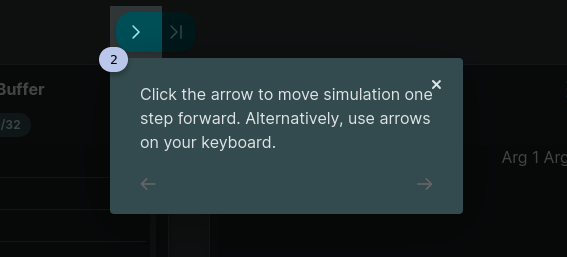
\includegraphics[width=11cm]{obrazky-figures/impl/Walkthrough.png}
    \caption{Průvodce základními funkcemi simulátoru.} 
    \label{walkthrough}
\end{figure}

% TODO Grafy vyhodnocení?

\section{Nasazení}
% build, dependencies

Aplikace je provozována kontejnery technologie Docker.
Docker jsem zvolil z~důvodů konzistence prostředí a jednoduchosti instalace.
První kontejner obsahuje webový server, druhý kontejner obsahuje simulační server.
Oba kontejnery ke komunikaci s~vnějškem otevírají jeden port.
Webový kontejner má síťový přístup do simulačního kontejneru, aby mohl předávat požadavky uživatele.
Součástí repozitáře je skript, který oba kontejnery spustí pomocí \texttt{docker-compose}.

V~případě použití Dockeru je jediným požadavkem instalace Dockeru a internetové připojení.
Jako virtualizační technologie má provoz serveru v~Dockeru nezanedbatelný dopad na výkon, vždy je ale možné aplikaci nainstalovat přímo.

Přímá instalace je detailně dokumentovaná v~textových souborech, které jsou součástí repozitáře a také v příloze \ref{installSteps}.
Je možné se inspirovat i nahlédnutím do kontejnerizačních skriptů, které obsahují přesnou sekvenci příkazů k instalaci a spuštění.
Prerekvizitami jsou programy \emph{Node.js} (runtime pro JavaScript), Java runtime, systém pro automatizaci překladu Gradle a GCC pro RISC-V (\texttt{gcc-riscv-none-elf}).

Knihovní závislosti webové aplikace jsou spravovány systémem NPM\footnote{\url{https://www.npmjs.com/}} (Node Package Manager).
Soubory \texttt{package.json} a \texttt{package-lock.json} specifikují použité knihovny a jejich verze.
Při instalaci jsou závislosti staženy z~centrálního repozitáře.

Proces nasazení je \emph{automatizovaný} službou \emph{GitLab CI/CD}.
Soubor \texttt{.gitlab-ci.yml} v~kořeni projektu definuje předpisy akcí, které se mají spouštět při různých událostech v~repozitáři.
Pro každý commit se spouští testy.
Úspěšnost testů je zobrazena v~grafickém rozhraní GitLabu.
Při novém \emph{Pull Requestu} se spustí server s~aplikací pro otestování a zhodnocení vedoucím.

Konfigurace simulátoru je založena na souboru s~dvojicemi klíč-hodnota.
Existují dvě verze této konfigurace (vývojová a produkční).
Výběr probíhá při startu podle proměnných prostředí.
Parametry lze přepsat argumenty příkazové řádky.
Webová aplikace se konfiguruje proměnnými prostředí.
Jedinou relevantní konfigurací je adresa simulačního serveru.

    
\chapter{Závěr}

V~této práci byly prozkoumány některé známé metody efektivní implementace superskalárních procesorů.
Detailněji byla probrána instrukční sada RISC-V, kterou simulátor využívá.
Také byla uvedena teorie implementace webových aplikací s~přihlédnutím k~návrhu uživatelských rozhraní.

Byla provedena důkladná analýza stávajícího simulátoru, zhodnocení jeho kladů i nedostatků.
Na základě analýzy byla navržena mnohá zlepšení, jak z~pohledu implementace simulace, tak použitelnosti jeho rozhraní.

Z~mého pohledu nejdůležitější změnou je samotné přenesení simulátoru na webovou platformu.
Simulátor je nyní všem dostupný přímo z~prohlížeče.

Do rozhraní simulátoru se podařilo přidat režim příkazové řádky a HTTP server.
Důležitou součástí simulátoru je integrace s~překladačem GCC a nový parser assembleru, který umožňuje simulovat širokou škálu programů v~jazyce C.
Společně s~množstvím před-připravených příkladů to uživatelům umožňuje rychle experimentovat se složitějšími programy, než jaké by mohli nebo chtěli psát ručně.
Simulátor také sbírá běhové statistiky a je možné definovat data, nad kterými má program pracovat.

Bylo také provedeno mnoho změn vnitřního fungování simulátoru.
Projekt obsahuje množství testů, dokumentace a skriptů k~instalaci, spuštění a nasazení do provozu.
Příloha \ref{prevzanaPrace} uvádí tabulku s~přehledem jednotlivých modulů aplikace a můj přínos.

Aplikace je v~současné podobě dobře provozuschopná, o~čemž svědčí kladný ohlas z~uživatelského dotazníku.
Na webové stránce je možné provozovat interaktivní simulaci, měnit konfiguraci, editovat kód a prohlížet statistiky o~simulaci.
Grafické zpracování a provázání prvků v~simulátoru přináší studentům přehledný zdroj k~výuce fungování moderních procesorů.

Přínos projektu pro výuku hardwaru vnímám velmi pozitivně.
Doufám, že aplikace najde své využití nejen na FIT VUT v~Brně, ale i v~široké studentské komunitě.

Budoucí práce se může zaměřit na další rozšíření instrukční sady, například na vektorové instrukce.
Dalším zajímavým směrem může být možnost programovatelného přerušení simulace v~určitém bodě (\emph{breakpoint}).

  \fi
  
  % Kompilace po částech (viz výše, nutno odkomentovat a zakomentovat input výše)
  % Compilation piecewise (see above, it is necessary to uncomment it and comment out input above)
  %\subfile{chapters/projekt-01-uvod-introduction}
  % ...
  %\subfile{chapters/projekt-05-zaver-conclusion}

  % Pouzita literatura / Bibliography
  % ----------------------------------------------
\ifslovak
  \makeatletter
  \def\@openbib@code{\addcontentsline{toc}{chapter}{Literatúra}}
  \makeatother
  \bibliographystyle{bib-styles/Pysny/skplain}
\else
  \ifczech
    \makeatletter
    \def\@openbib@code{\addcontentsline{toc}{chapter}{Literatura}}
    \makeatother
    \bibliographystyle{bib-styles/Pysny/czplain}
  \else 
    \makeatletter
    \def\@openbib@code{\addcontentsline{toc}{chapter}{Bibliography}}
    \makeatother
    \bibliographystyle{bib-styles/Pysny/enplain}
  %  \bibliographystyle{alpha}
  \fi
\fi
  \begin{flushleft}
  \bibliography{projekt-20-literatura-bibliography}
  \end{flushleft}

  % vynechani stranky v oboustrannem rezimu
  % Skip the page in the two-sided mode
  \iftwoside
    \cleardoublepage
  \fi

  % Prilohy / Appendices
  % ---------------------------------------------
  \appendix
\ifczech
  \renewcommand{\appendixpagename}{Přílohy}
  \renewcommand{\appendixtocname}{Přílohy}
  \renewcommand{\appendixname}{Příloha}
\fi
\ifslovak
  \renewcommand{\appendixpagename}{Prílohy}
  \renewcommand{\appendixtocname}{Prílohy}
  \renewcommand{\appendixname}{Príloha}
\fi
%  \appendixpage

% vynechani stranky v oboustrannem rezimu
% Skip the page in the two-sided mode
%\iftwoside
%  \cleardoublepage
%\fi
  
\ifslovak
%  \section*{Zoznam príloh}
%  \addcontentsline{toc}{section}{Zoznam príloh}
\else
  \ifczech
%    \section*{Seznam příloh}
%    \addcontentsline{toc}{section}{Seznam příloh}
  \else
%    \section*{List of Appendices}
%    \addcontentsline{toc}{section}{List of Appendices}
  \fi
\fi
  \startcontents[chapters]
  \setlength{\parskip}{0pt} 
  % seznam příloh / list of appendices
  % \printcontents[chapters]{l}{0}{\setcounter{tocdepth}{2}}
  
  \ifODSAZ
    \setlength{\parskip}{0.5\bigskipamount}
  \else
    \setlength{\parskip}{0pt}
  \fi
  
  % vynechani stranky v oboustrannem rezimu
  \iftwoside
    \cleardoublepage
  \fi
  
  % Přílohy / Appendices
  \ifenglish
    \input{projekt-30-prilohy-appendices-en}
  \else
    
\chapter{Přehled převzaté práce}
\label{prevzanaPrace}

V této příloze je uveden rozpis jednotlivých modulů a míra, do které jsem k implementaci modulu přispěl.

\begin{table}[h]
\centering
\begin{tabular}{|l|c|c|c|c|}
\hline
Modul                      & Původní & Refaktorizován & Značně upraven & Nový \\ \hline
\hline
Rozhraní procesoru         &         &                & \checkmark              &      \\ \hline
Registry a registrové pole &         &                & \checkmark              &      \\ \hline
Fáze Fetch, Decode         &         & \checkmark              &                &      \\ \hline
ROB                        &         & \checkmark              &                &      \\ \hline
Fáze Execute               &         & \checkmark              &                &      \\ \hline
Reprezentace instrukcí     &         &                & \checkmark              &      \\ \hline
Interpretace instrukcí     &         &                & \checkmark              &      \\ \hline
Paměti a cache             &         & \checkmark              &                &      \\ \hline
Alokace polí v paměti      &         &                &                & \checkmark    \\ \hline
Parsování a překlad kódu   &         &                &                & \checkmark    \\ \hline
Nastavení simulace         &         &                & \checkmark              &      \\ \hline
Sběr statistik             &         &                & \checkmark              &      \\ \hline
Server, serializace        &         &                &                & \checkmark    \\ \hline
Předpověď skoků            &         & \checkmark              &                &      \\ \hline
Instrukční sada RISC-V     &         &                & \checkmark              &      \\ \hline
Testy                      &         &                & \checkmark              &      \\ \hline
Webové rozhraní            &         &                &                & \checkmark    \\ \hline
Kontejnerizace             &         &                &                & \checkmark    \\ \hline
\end{tabular}
\caption{Přehled modulů a můj přínos implementaci.}
\label{myworkTable}
\end{table}

  \fi
  
  % Kompilace po částech (viz výše, nutno odkomentovat)
  % Compilation piecewise (see above, it is necessary to uncomment it)
  %\subfile{projekt-30-prilohy-appendices}
  
\end{document}
